% !TEX program = xelatex
\documentclass[
  10pt,
  twoside,
  openany,
  b5paper, % 以上均为 ctexbook 提供的文类选项
  colorscheme = basic, % 请根据需要选择或定制配色方案
  noCJKfont
]{qyxf-book}

\ctexset{fontset = fandol}

\usepackage{mathtools}
\usepackage[figuresright]{rotating}
\usepackage{multirow}
\usepackage{multicol}
\usepackage{threeparttable}

\newtheorem{defn}{定义}[chapter]
\newtheorem{exam}{例}[chapter]
\newtheorem{prop}{命题}[chapter]

\newcommand{\tabincell}[2]{\begin{tabular}{@{}#1@{}}#2\end{tabular}}


\title{图模型、指数族与变分推断}
\subtitle{Graphical Models, Exponential Families, and Variational Inference}  % 可选
\author{朱明仁(译)}
\date{\today}
%\typo{AlphaGo}  % 排版人员信息,选填

% 定制元信息
\org{\Large\textit{北京理工大学}\\\textsc{Beijing Institute of Technology}}
\footorg{\textsc{Keep learning.}}
\cover{\vspace{6cm}
\includegraphics[width=.4\textwidth]{bit_logo.pdf}}
\license{}  % 清空许可证信息

% 调整封面标题大小
\renewcommand{\titlefont}{\Huge\bfseries}
\renewcommand{\subtitlefont}{\LARGE\itshape}

\begin{document}

\maketitle

\tableofcontents

\chapter*{摘 \quad 要}
\addcontentsline{toc}{chapter}{\textbf{摘 \quad 要}}

概率图模型(Probabilistic graphical models, PGMs)这一形式化工具为捕获随机变量之间复杂的依赖性从而建立大规模多变量统计模型提供了一个统一的框架。
在统计、计算机与数学的众多领域中,图模型已经成为了一个研究的热点,包括生物信息、通讯理论、统计物理、组合优化、信号和图像处理、信息检索以及统计机器学习等。
许多从特例中发现的问题,例如边缘分布与众数的计算,已经在一般条件下得到了很好的研究。
我们使用指数族分布(Exponential families)进行概率表示,利用指数族的累积函数(Cumulant function)和熵(Entropy)的共轭对偶性(Conjugate duality),提出了一套可用于计算似然(Likelihoods)、边缘概率(Marginal probabilities)和最概然配置(Most probable configurations)的通用变分表示方法(Variational representations)。
我们对一大群算法变体进行了描述,包括和积算法(Sum-product)、聚类变分法(Cluster variational methods)、期望传播算法(Expectation-propagation)、平均场方法(Mean field methods)、最大积算法(Max-product)、线性规划松弛法(Linear programming relaxation)以及二次规划松弛法(Conic programming relaxation),这些算法都可以理解为是变分表示的精确或近似形式。
变分方法为大规模统计模型的近似推断提供了与马尔可夫链蒙特卡洛法(Markov Chain Monte Carlo, MCMC)完全互补的另一项选择。

\chapter{引言}

图模型将图论和概率论结合在一起,构成了一个用于多变量统计建模的强大形式框架。
在包括生物信息、语音处理、图像处理和控制论等多个应用领域内,统计模型早已习惯于使用图来进行形式化表达,而计算如似然和得分函数等基本统计量的算法也常被表示为在这些图上的递归操作,例如物种进化树、遗传图谱、隐马尔可夫模型、马尔可夫随机场以及卡尔曼滤波等。
这些想法都能使用图模型的形式进行理解、统一和泛化。
图模型不仅提供了一种很自然的工具来阐述这些经典结构的变体,还可以用于探索全新的统计模型族。
于是在涉及到需要研究大量有交互作用的变量的领域,图模型的使用频率在显著地升高。

在许多面向计算的领域里,图论扮演了十分重要的一个角色,包括组合优化、统计物理和经济学等。
除了可以用来形式化模型之外,图论也在评价计算的复杂度和灵活度中起到了基础性的作用。
特别地,一个算法的运行时长或者是误差界的量级也经常能够表示为某个图的结构特征。
图论起到的这种作用在图模型中也同样存在。
例如我们之后会讨论的名为“联合树算法”(Junction tree algorithm)——一种上文提到的在图上的递归算法的一般化版本——的计算复杂度就能够用相互作用的变量所构成的图的理论度量来表示。
对于某些特殊的稀疏图,联合树算法提供了一套系统的方案可以用来计算图模型上的似然和其他统计量。

不幸的是,许多实际的图模型并不是稀疏的,所以联合树算法不能提供可行的计算方案。
MCMC 框架是一种很受欢迎的方法,可以用来解决上面那种情况,大量的文献都在图模型上应用了 MCMC 方法。
然而我们的目标有些不一样:我们提出另一种基于变分方法的统计推断计算方法论。
这项技术不仅提供了 MCMC 的替代品,还具有在图模型框架之外的应用。
然而我们将会看到变分方法能够很自然地运用到图模型中去,因为变分方法和图的结构属性有着密切的联系。

“变分”本身是一个概括性的词汇,指的是把问题用优化的形式进行表达和求解的各种数学工具。
一般的想法是把感兴趣的量表示为一个优化问题的解。
优化问题可以通过不同的方式放宽约束条件,可以对优化目标函数进行近似处理,也可以对可行域进行近似处理。
这些放宽约束的手段提供了一种原问题的近似方法。

MCMC 和变分方法都来自于统计物理。
MCMC 方法在进入统计领域之前就已经在统计物理中取得了很好的应用效果,这也促进了统计领域对这一方法的理论研究。
事实上,为特定统计问题所设计的 MCMC 方法的发展为此类方法在统计领域的广泛应用起到了重要作用。
变分方法可以借鉴这种发展方式,在我们看来,将变分方法应用到统计领域最有希望的途径是利用好变分分析和指数族分布之间的联系上。
这是因为处于指数族统计理论核心位置的凸性概念对变分松弛的设计有很大的作用。
此外,这些变分松弛法在图模型的结构上可以产出很有意思的算法,这些算法同样以在图上递归的形式实现。

我们对三个相关的主题呈现了一个完整的故事。
我们在第二章中讨论图模型,在提供一般的数学框架的同时也针对几个特例进行讲解。
所有这些例子以及当前图模型的大多数应用都涉及到指数族分布。
我们在第三章中讨论指数族,着重于指数族和凸分析之间的数学联系,在此基础上给出变分方法的发展脉络。
需要特别突出说明的是指数族的某种共轭对偶关系。
在共轭对偶关系的基础上,我们提出了用于计算指数族似然和边缘概率方法的一般变分表示。
随后的部分将致力于探索这个变分原理的各种实例,包括精确和近似形式,从中可以得到精确或近似计算边缘概率的各种算法。
我们在第四章中讨论贝特近似(Bethe approximation)与和积算法之间的联系,包括在树结构上的精确形式和在带环图结构上的近似形式。
我们也会讨论类贝特近似(Bethe-like approximation)与其他算法之间的联系,包括广义和积算法(Generalized sum-product)、期望传播算法以及相关的矩匹配(Moment-matching)方法。
我们在第五章中讨论平均场方法,这是一种不同于精确变分原理的近似方法,可以生成似然下界。
我们在第六章中讨论变分方法在参数估计中所起到的作用,包括全观测与部分观测两种情况的例子,也包括频率派和贝叶斯派两种不同的视角。
贝特型(Bethe-type)和平均场方法都是基于非凸优化问题的,这类问题经常有多重解。
相较之下我们在第七章中讨论基于精确变分原理凸松弛的变分方法,这类方法大多数都能保证对数似然存在上界。
我们在第八章中讨论众数(Mode)的计算问题,特别强调离散随机变量的情况,这种情况下计算众数需要解决一个整数规划问题(Integer programming problem)。
我们发展了(重新加权的)最大积算法与层次线性规划松弛之间的联系。
我们在第九章中讨论更为一般的二次规划松弛,并且从矩矩阵(Moment matrices)的半定约束(Semi-definite constraints)的视角来进行理解。
我们在第十章进行总结。

这篇文章的范围限于以下情形:给定表示为图模型的一个概率分布,我们主要关心计算边缘概率(包括似然)和众数的问题。
我们习惯上将这种计算任务称为“概率推断”或者简称“推断”。
正如 MCMC 方法的介绍一样,我们关注的主要是贝叶斯统计中的应用。
虽然贝叶斯统计在我们的介绍中占主要部分,但是这些方法可以运用到整个统计范围中去,包括频率和贝叶斯两种范式,我们在这篇文章中指出了一些交叉性的应用。



\chapter{图模型背景}

我们从图模型的研究背景开始讲解。
最关键的想法是因子分解:一个图模型由可以根据图结构进行因子分解的一系列概率分布构成。
这里的“分布”是不精确的,$p$ 应该被理解为是一个离散的质量函数(计数测度上的密度),或者是连续情况下勒贝格测度的密度。
本章节主要讲解条件独立性(Conditional independence)等概率概念与团(Cliques)、分割(Separation)等图论概念之间的相互关系。

\section{图结构表示的概率分布}

我们首先描述几类有用的图形式。
一个图 $G = (V, E)$ 是由一系列顶点 $V = \{1, 2, \dots, m\}$ 和一系列连边 $E \subset V \times V$ 构成的。
每一条边都连接一对顶点 $s, t \in E$,无向边代表 $(s, t)$ 和 $(t, s)$ 之间并没有什么不同,而有向边可以写为 $(s \rightarrow t)$ 来表达方向。
附录 A.1 有关于图及其性质更多的介绍。

为了定义一个图模型,我们把每个节点 $s \in V$ 都赋予一个从某个空间 $\mathcal{X}_s$ 中取值的随机变量 $X_s$。
取决于具体的应用情况,状态空间 $\mathcal{X}_s$ 既可以是连续的($\mathcal{X}_s = \mathbb{R}$)也可以是离散的($\mathcal{X}_s = \{0, 1, \dots, r-1\}$)。
我们使用小写字母($x_s \in \mathcal{X}_s$)来表示 $\mathcal{X}_s$ 中的特定元素,因此 $\{X_s = x_s\}$ 代表随机变量 $X_s$ 取值为 $x_s \in \mathcal{X}_s$ 的事件。
对于任意的节点子集 $A \subset V$,我们定义子集随机向量 $X_A \coloneqq (X_s, s \in A)$,其对应的取值向量可以表示为 $x_A \coloneqq (x_s, s \in A)$。
同样地,我们定义 $\otimes_{s \in A}\mathcal{X}_s$ 为 $X_A$ 中每个元素状态空间的笛卡尔积。

\subsection{有向图模型}

给定一个带有边 $(s \rightarrow t)$ 的有向图,我们称 $t$ 是 $s$ 的一个子节点,或者相对地,$s$ 是 $t$ 的一个父节点。
对于任意节点 $s \in V$,它的所有父节点构成的集合表示为 $\pi(s)$。
(如果节点 $s$ 没有父节点,那么 $\pi(s)$ 代表空集。)
一个有向环是指一条序列 $(s_1, s_2, \dots, s_k)$,其中对于 $i = 1, \dots, k-1$ 都有 $(s_i \rightarrow s_{i+1}) \in E$,并且 $(s_k \rightarrow s_1) \in E$。
图 \ref{fig:2-1} 对这些概念进行了直观解释。

\begin{figure}[htbp]
    \centering
    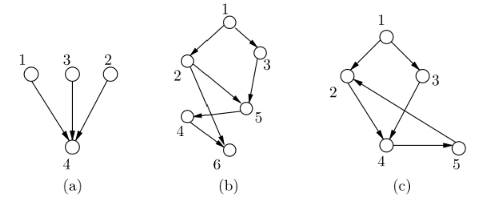
\includegraphics[width=.8\linewidth]{2-1.PNG}
    \caption{
        (a) 一个简单的带有四个变量 $(X_1, X_2, X_3, X_4)$ 的有向图模型。
        节点 $\{1, 2, 3\}$ 是节点 $4$ 的父节点,写作 $\pi(4) = \{1, 2, 3\}$。
        (b) 一个更复杂的有向无环图,定义了其节点的一个偏序(Partial order)结构。
        注意到节点 $6$ 是节点 $2$ 的一个子节点,节点 $1$ 是节点 $6$ 的一个祖先(Ancestor)。
        (c) 一个禁忌的有向图模型(带有环),其中包含了一个有向环路 $(2 \rightarrow 4 \rightarrow 5 \rightarrow 2)$。
    }\label{fig:2-1}
\end{figure}

假设 $G$ 是一个有向无环图(Directed acyclic graph,DAG),这意味着所有的连边都是有向的,并且图上不含有向环路。
对于任意一个 DAG,我们可以通过祖先的概念定义节点集 $V$ 的一个偏序结构:如果存在一条有向路径 $(s, t_1, t_2, \dots, t_k, u)$,则称节点 $s$ 是节点 $u$ 的一个祖先(见图 \ref{fig:2-1}(b))。
给定一个 DAG,对于每一个节点 $s$ 和它的父节点 $\pi(s)$,以 $p_s(x_s|x_{\pi(s)})$ 表示一个定义在变量 $(x_s, x_{\pi(s)})$ 上的非负函数,并且满足归一化条件 $\int p_s(x_s|x_{\pi(s)})dx_s = 1$。
就这些局部函数而言,有向图模型由一系列概率分布(密度或质量函数)组成,这些概率分布可以按照以下方式进行分解:

\begin{equation}
    p(x_1, x_2, \dots, x_m) = \prod_{s \in V}p_s(x_s|x_{\pi(s)})
\end{equation}

在这里,符号的使用与一般习惯是一致的,事实上 $p_s(x_s|x_{\pi(s)})$ 就代表着由因子分解 (2.1) 所表示的分布 $p(\cdot)$ 在给定 $\{X_{\pi(s)} = x_{\pi(s)}\}$ 的情况下 $\{X_s = x_s\}$ 的条件概率。
这是一个可以利用 $p_s(\cdot)$ 的归一化条件和 DAG 上由祖先关系导出的偏序结构所得到的归纳结论。

\subsection{无向图模型}

在无向的情形下,概率分布可以根据定义在图上的团(Cliques)结构进行因子分解。
一个团 $C$ 是指节点集 $V$ 的一个全连接子集,意味着对于所有 $s, t \in C$ 都有 $(s, t) \in E$。
我们在每个团结构 $C$ 上都定义一个势函数(Compatibility function) $\psi_C: (\otimes_{s \in C}\mathcal{X}_s) \rightarrow \mathbb{R}_+$。
注意 $\otimes_{s \in C}\mathcal{X}_s$ 表示随机向量 $X_C$ 状态空间的笛卡尔积。
因此势函数 $\psi_C$ 是一个仅仅定义在团元素上的局部量。

使用这些记号一个无向图模型——或者说马尔可夫随机场(Markov random field, MRF),又或者说吉布斯分布(Gibbs distribution)——是一系列能够进行以下分解的分布:

\begin{equation}
    p(x_1, x_2, \dots, x_m) = \frac{1}{Z}\prod_{C \in \mathcal{C}}\psi_C(x_C)
\end{equation}

其中 $Z$ 是归一化常数。
$\mathcal{C}$ 经常取为图上所有的最大团(Maximal cliques)组成的集合,也就是不属于任何其他团的团所构成的集合。
这个条件可以保证不失一般性,因为任何基于非最大团的表示总是可以转化为基于最大团的表示,只需要重新定义最大团上的势函数,使之成为该团子集上的势函数的乘积即可。
然而,使用非最大团的表示可能带来计算的简便性,尤其是在算法可以利用基于非最大团的因子分解的特点的时候。
因此,我们不必将势函数限制在最大团上,而是将集合 $\mathcal{C}$ 定义为可以包含任何团结构。
(在下一节讨论的因子图将会对分解属性提出更细致的规范。)

必须理解的是,对于一个一般的无向图而言,势函数 $\psi_C$ 并不需要与定义在团上的边缘或条件分布有任何明显或直接的关系。
这个属性与有向图的因子分解形成了对比,在有向图中因子对应着父子节点之间的条件概率。

\subsection{因子图}

对于大规模的图而言,无论是有向图还是无向图,它的因子分解都很难从图的通常描述中观察得到。
因子图(Factor graphs)的形式提供了图的另一种表示方法,主要强调对分布的分解。

令 $F$ 为定义在图模型分布上的因子的索引集。
在无向图的情况下,$F$ 索引了 $\mathcal{C}$ 中的团结构,在有向图的情况下则索引了父子节点集。
接下来我们考虑一个二分图 $G' = (V, F, E')$,其中 $V$ 还是原来的节点集合,$E'$ 是一个新的边集合,连接节点 $s \in V$ 和因子 $a \in F$。
特别地,$(s, a) \in E'$ 当且仅当 $x_s$ 存在于由 $a \in F$ 索引的因子中。
参见图 \ref{fig:2-2}(b)。

\begin{figure}[htbp]
    \centering
    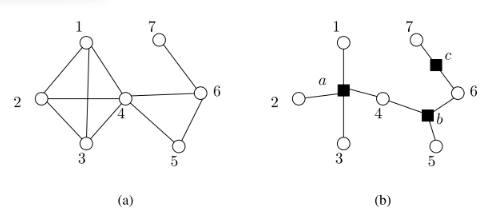
\includegraphics[width=.8\linewidth]{2-2.PNG}
    \caption{
        无向图和因子图。
        (a) 7个节点上的无向图,拥有最大团 $\{1, 2, 3, 4\}$,$\{4, 5, 6\}$ 和 $\{6, 7\}$。
        (b) (a) 中无向图等价的因子图表示,假设我们只在最大团上定义了势函数。
        因子图是一个二部图,拥有节点集 $V = \{1, \dots, 7\}$ 和因子集 $F = \{a, b, c\}$,每个因子对应原无向图上的一个势函数。
    }\label{fig:2-2}
\end{figure}

对于无向图模型来说,当 $\mathcal{C}$ 包含不仅仅只是最大团时,因子图表示具有特殊的价值。
事实上在一般的无向图表示中,非最大团的势函数并没有明显的表示出来,而因子图可以让它们显性化。

\section{条件独立性}

由式 (2.1) 和式 (2.2) 定义的概率分布族在随机变量的子集之间存在着条件独立性的特征——原图模型的马尔可夫性(Markov properties)。
我们在这里只粗略过一下这个特性,因为在文章其他部分并没有涉及到太多相关的内容。
如果读者对此有兴趣,我们推荐可以去看一下 Lauritzen 的作品。

对于无向图模型而言,条件独立性与图论中的可达性概念相一致。
特别地,令 $A$,$B$ 以及 $C$ 是互不相交的节点子集三元组。
如果删掉节点集 $C$ 之后没有任何一条路径能够从 $A$ 到达 $B$,那么我们称在给定 $X_C$ 的条件下 $X_A$ 与 $X_B$ 是独立的。
在子集 $A$,$B$ 以及 $C$ 的所有可能选择范围内可以产出一个条件独立性列表。
这些列表总是自洽的(即存在满足这些列表中所有条件独立性的概率分布),而且符合条件的概率分布集正是由式 (2.2) 所定义的分布集,涵盖了势函数的所有可能选择。

因此与无向图相关的概率分布族有两种等价刻画。
这个等价性是一个基本的数学结论,连接了一个代数概念(因子分解)和一个图论概念(可达性)。
这一结论也产出了一个可以用来检验条件独立性的算法,因为它将条件独立性的评估问题简化为图上可达性的评估问题。
这很容易用图上的广度优先搜索来解决。

在有向图模型中也有类似的结果,唯一的变化是可达性的概念。
同样,在有向图的因子分解 (2.1) 中指定的概率分布族与根据一组条件独立性所定义的概率分布族之间建立等价关系是可能的。

\section{统计推断和精确算法}

给定一个定义在图模型上的概率分布 $p$,我们主要关注解决以下一个或多个计算推断问题(Computational inference problems):

\begin{enumerate}
    \item[(1)] 计算观测得到的数据的似然。
    \item[(2)] 计算特定子集 $A \subset V$ 的边缘分布 $p(x_A)$。
    \item[(3)] 计算不相交子集 $A$ 和 $B$ 的条件分布 $p(x_A|x_B)$。
    \item[(4)] 计算密度的众数($\hat{x} = arg\max_{x \in \mathcal{X}}p(x)$)。
\end{enumerate}

显然问题 (1) 是问题 (2) 的一个特例。
(3) 中条件概率的计算似乎也是需要边缘化的步骤,首先需要得到分子 $p(x_A, x_B)$,然后需要得到分母 $p(x_B)$。
相较而言,(4) 中关于众数的计算从基础上就是不同的,因为它涉及最大化而不是积分的问题。
尽管如此,我们后续所提出的变分方法将会突出某些计算边际与计算众数的重要联系。

为了理解这些推断问题的内在挑战,考虑一个离散随机向量的例子 $x \in \mathcal{X}^m$,其中对于每个节点 $s \in V$ 都有 $\mathcal{X}_s = \{0, 1, \dots, r-1\}$。
在单个节点上计算边际 $p(x_s)$,一种朴素的方法是对所有的 $\{x' \in \mathcal{X}^m|x_s' \neq x_s\}$ 进行求和。
这个集合一共有 $r^{m-1}$ 个元素,很明显很难用暴力方法来处理这种问题。
即使是二元变量($r = 2$)和一个 $m \approx 100$ 个节点的图(对于很多应用程序来说规模很小),这个求和也超出了暴力计算的能力范围。
类似地,在这个离散地情况下计算一个众数需要在一个指数量级地可行解空间解决一个整数规划问题。
对于连续随机变量,问题并不会得到简化 \footnote{高斯情况是一个特例} 而通常会更难,因为它们需要计算大量的积分。

对于没有环的无向图和每个节点只有一个父节点的有向图——也就是树——来说,这些推断问题都能够利用自然的动态规划性质使用“消息传递(Message-passing)”递归算法得到精确的解决,计算复杂度只是节点数量的线性量级。
特别地,在计算边际的情况下,动态规划将会退化为另一种一般算法的形式,称为和积算法(Sum-product),而对于计算众数的问题则退化为另一种相似的最大积算法(Max-product)。
我们将在 2.5.1 小节描述这些算法。
更一般地说,正如我们将在 2.5.2 小节中讨论的,联合树算法(Junction tree)为任意图的推断问题提供了一种解决方案。
联合树算法的计算复杂度的指数级的,底数为图的树宽(Treewidth)。

\section{应用}

在转向算法问题的研究之前,我们最好先广泛地讨论一下各种图模型的应用实例。
我们展示了几个一般场景下的图模型应用实例,包括贝叶斯层次建模、列联表分析、组合优化和可满足性等一般领域中使用图模型的例子,以及在生物信息学、语音和语言处理、图像处理、空间统计、通信和编码理论中的具体例子。

\subsection{贝叶斯层次建模}

贝叶斯框架把所有模型量都作为随机变量,包括观测数据、隐变量、参数、干扰变量等。
因此图模型表示下的贝叶斯模型,所有这些变量都以节点的身份出现在图中。
与图模型相关的通用计算方法可以直接应用于参数的边际和后验概率等贝叶斯量的计算。
尽管贝叶斯模型能够使用有向或无向图两种进行表示,实践中所遇到的大多数还是以有向图为主。
特别地,在贝叶斯层次模型中,先验分布的定义通常涉及额外的参数,称为超参数,而整个模型被定义为一组连接超参数、参数和数据的条件概率。
把这些条件概率分布做乘积就得到了联合概率分布,这种因子分解只是式 (2.1) 的一个简单实例而已。

把贝叶斯层次模型当作有向图模型看待有几点好处。
第一,层次模型通常通过对条件独立性的各种说明来指定。
这些说明暗含了其他条件独立性关系,而且可达性算法也提供了一种系统性的方法来验证这些关系。
第二,由图提供的可视化既能帮助理解模型(包括验证图无环的基本步骤),也更有利于进行扩展和探索。
最后,一般的计算方法如 MCMC 和变分推断算法等都能够应用在图模型上,因此就需要把层次模型表达为图的形式。
这些方便之处促进了通过有向图形式来操作贝叶斯层次模型的通用软件程序的发展。

\subsection{列联表分析}

列联表是一种应用于多类型数据分析中的核心工具,可以追溯到 Pearson、Yule 和 Fisher 的开创性研究。
一个 $m$ 维的,每个维度都有 $r$ 个水平的列联表表示一个定义在 $m$ 个随机变量 $(X_1, \dots, X_m)$,每一个随机变量都有 $r$ 个可能取值的概率分布。
举个具体的例子 $m = 2$,一个具有 $r$ 个水平的列联表是一个简单的 $r \times r$ 的元素非负的加和为 $1$ 的矩阵,对于 $m > 2$ 来说则是一个具有 $r^m$ 个非负元素且加和为 $1$ 的多维数组。
因此,这个表完整地确定了一个定义在随机向量 $(X_1, \dots, X_m)$ 上的,每个随机变量 $X_s$ 取 $r$ 个可能取值的概率分布。

列联表可以使用图模型的框架进行建模,而且图的形式给许多自然的问题提供了一种很有帮助的可视化。
例如,在列联表分析中一个核心问题是区分数据中不同的交互顺序。
作为一个具体的例子,给定 $m = 3$ 个变量,一个简单的问题是测试这三个变量之间是否独立。
从图模型的角度来看,这个测试相当于在相关的交互图上连接是否是全部断开的(见图 \ref{fig:2-3}(a)(b))。
一个更微妙的测试是区分随机变量是否仅以成对的方式相互作用(用式 (2.2) 来说就是只有因子 $\psi_{12}$,$\psi_{13}$ 以及 $\psi_{23}$),又或者实际上是三方交互作用(式 (2.2) 中仅有 $\psi_{123}$)。
有趣的是这两种因子分解的方式是没办法用标准的无向图来进行区分的,如图 \ref{fig:2-3}(b) 所示,3 个节点的全连接图是不区分三重交互作用与成对交互作用的。
这么看来因子图的形式更为有效,因为它是能够区分成对交互和三重交互的,如图 \ref{fig:2-3}(c)(d) 所示。

\begin{figure}[htbp]
    \centering
    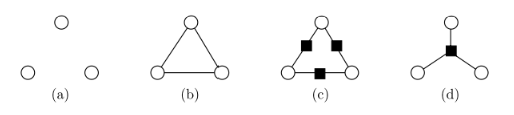
\includegraphics[width=.8\linewidth]{2-3.PNG}
    \caption{
        列联表分析中一些简单的图交互作用。
        (a) 独立模型。
        (b) 一般的非独立模型。
        (c) 只有成对交互作用。
        (d) 三重交互作用。
    }\label{fig:2-3}
\end{figure}

\subsection{约束满足和组合优化}

约束满足和组合优化问题出现在各种各样的领域,其中包括人工智能、通信理论、计算复杂性理论、统计图像处理和生物信息学。
可满足性和组合优化中的许多问题都是用图论的术语定义的,因此很自然地以图模型的形式进行重塑。

让我们考虑一个可能是最著名的可满足性的例子,即 3-SAT 问题。
它可以很自然地用因子图和二元随机变量 $(X_1, X_2, \dots, X_m) \in \{0, 1\}^m$ 来表示。
对于一个给定的节点三元组 $\{s, t, u\}$,我们首先定义一些“禁忌”的模式 $(z_s, z_t, z_u) \in \{0, 1\}^3$,然后再定义三元组的势函数

\begin{equation}
    \psi_{stu}(x_s, x_t, x_u) = \begin{cases}
        0 & \text{如果} (x_s, x_t, x_u) = (z_s, z_t, z_u) \\
        1 & \text{其他}
    \end{cases}
\end{equation}

每个这样的势函数在可满足性的文献中被称为子句,通常按照逻辑操作进行编码。
举个具体的例子,如果 $(z_s, z_t, z_u) = (0, 0, 0)$,那么式 (2.3) 就能被简洁地写为 $\psi_{stu}(x_s, x_t, x_u) = x_s \vee x_t \vee x_u$,其中 $\vee$ 代表两个布尔符号间的逻辑或操作。

作为一个图模型,图 \ref{fig:2-3}(d) 和一个单子句相关,让人更感兴趣的是建立在更大规模的二元变量集之上的模型,其中包含许多子句。
在可满足性上的一个基本问题是判断给定的一个子句集合 $F$ 是否是可满足的,这意味着存在某种配置 $x \in \{0, 1\}^m$ 使得 $\prod_{(s, t, u) \in F}\psi_{stu}(x_s, x_t, x_u) = 1$。
在这种情况下,因子分解 $$p(x) = \frac{1}{Z}\prod_{(s, t, u) \in F}\psi_{stu}(x_s, x_t, x_u)$$ 定义了在满足的配置集合上的均匀分布。

如果 3-SAT 的实例是随机构建的——例如固定一个子句密度 $\alpha > 0$,然后从 $m$ 个变量组成的三元组中随机抽取 $\lceil\alpha m \rceil$ 个子句——图的形式将会趋向于一种局部的“类树”结构,参见图 \ref{fig:2-9}(b)。
这个问题上存在一个临界点 $\alpha^*$,当 $\alpha$ 小于这个值的时候基本没什么约束,而当 $\alpha$ 足够大的时候基本就是不可满足的,这种相变的现象是相关研究中的一个重要问题。

调查传播算法(Survey propagation)是解决随机可满足性问题的一种很有前景的方法,它是从统计物理领域发展起来的。
已经有研究表明调查传播算法是和积算法或者信念传播算法在以图模型表示的可满足性问题上的一个特例。

\subsection{生物信息学}

生物信息学中的许多经典模型都是图模型的实例,图模型的相关框架也常被用来设计新的模型。
本小节我们简单回顾一些在生物信息学中所应用到的经典的或者最近的图模型例子。
序列数据在生物信息学领域有着十分重要的地位,图 \ref{fig:2-4}(a) 所示的隐马尔可夫模型(Hidden markov model, HMM)是对序列数据进行处理的一个基础模型。
HMM 本质上是有限混合模型的一个动态版本,这类模型都假设观测数据是在一个隐状态下产生的。
状态变量通常是服从多项式分布的离散随机变量,在时序上构成马尔可夫链。
图 \ref{fig:2-4}(a) 表示的图模型同样也是基于卡尔曼滤波(Kalman filter)的状态—空间模型(State-space model),这个模型下的状态变量是一个高斯向量。
这个模型同样也可以被称为是“隐马尔可夫模型”,只不过这个名称通常是指状态变量取离散值的模型。

\begin{figure}[htbp]
    \centering
    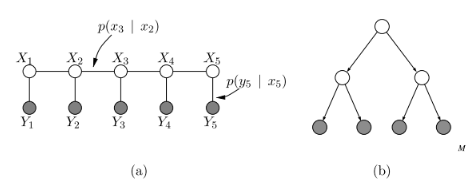
\includegraphics[width=.8\linewidth]{2-4.PNG}
    \caption{
        (a) 一般隐马尔可夫模型的图表示。
        阴影节点 $\{Y_1, \dots, Y_5\}$ 代表观测变量,非阴影节点 $\{X_1, \dots, X_5\}$ 代表隐状态变量。
        后者构成了一条马尔可夫链,在给定 $X_t$ 的条件下 $X_s$ 独立于 $X_u$,其中 $s < t < u$。
        (b) 在四个现存的有机体和 $M$ 位点上的物种演化的图表示。
        这棵树诠释了这么一种假设:首先有一个物种形成事件,随后有两个进一步的物种形成事件,最终形成了现存的四种生物。
    }\label{fig:2-4}
\end{figure}

将联合树算法应用到 HMM 上产生了一种新的算法,新算法沿着状态变量链在两个方向上进行消息传递,以此计算边际概率 $p(x_t, x_{t+1}|y)$ 和 $p(x_t|y)$。
这套消息传递算法在 HMM 中被称为前后向算法(Forward-backward algorithm)。
这些边际概率的推断过程本身很有趣,而在对 HMM 进行参数估计的时候,这些边际概率在所使用的期望最大化(Expectation-maximization,EM)算法中也扮演着充分统计量的重要作用。
类似地,最大后验状态序列也能通过联合树算法计算出来(用最大化代替求和)——这个算法在 HMM 中被称为维特比算法(Viterbi algorithm)。

基因发现是 HMM 的一个应用场景。
粗略地说,一个有机体的基因组序列可以分为包含基因的区域和基因间的区域(分离基因),其中基因作为一段核苷酸序列,可以进一步地分为有意义的基因内结构(外显子和内含子)。
这些区段之间的边界是高度随机的,因此很难可靠地把它们找出来。
HMM 是解决这一问题的方法之一,设计者可以将有关基因结构的生物学知识编码进状态和状态转移过程。
HMM 也可以用来为蛋白质结构进行建模。
例如,膜蛋白是一种特殊的蛋白质,它们嵌入到细胞膜中,在细胞内外信号的传递中起着重要的作用。
这些蛋白质多次进出细胞膜,在亲水基性氨基酸和疏水基性氨基酸之间交替。
这些生物学知识被用来设计跨膜 HMM(一种建模膜蛋白的 HMM 模型)的状态和状态转移矩阵。

树结构模型在生物信息学和语言处理中也发挥着重要作用。
例如物种演化树可以看作图模型。
如图 \ref{fig:2-4}(b) 所示,物种演化树是一种树结构的图模型,其中一组观察到的核苷酸(或者其他生物学特征)假定是从一组潜在的祖先物种进化而来。
树中的条件概率是通过进化替代模型得到的,而可能性的计算是通过在树上进行递归剪枝来实现的。
这种递归是联合树算法的一个特例。

图 \ref{fig:2-5} 展示了一些在生物信息学中被应用的更为复杂的图模型。
图 \ref{fig:2-5}(a) 展示了隐马尔可夫物种演化模型,其中观察到的是一组与物种演化树相关的核苷酸。
基于多种灵长类动物的数据,这一模型已被证明对人类基因组的基因发现很有作用。
图 \ref{fig:2-5}(b) 展示了因子隐马尔可夫模型,其中多个链通过与一组共同的观察变量相连接而耦合。
这个模型抓住了遗传学中的多位点连锁分析的问题,其中状态变量对应于减数分裂时染色体上的相位。

\begin{figure}[htbp]
    \centering
    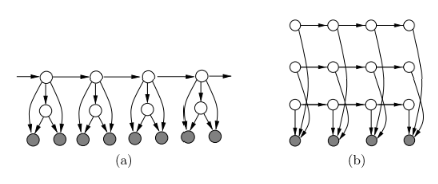
\includegraphics[width=.8\linewidth]{2-5.PNG}
    \caption{
        应用在生物信息学上的 HMM 的变体。
        (a) 物种演化 HMM。
        (b) 因子 HMM。
    }\label{fig:2-5}
\end{figure}

\subsection{语言和语音处理}

在语言问题中,HMM 也扮演着一种基础角色。
一个例子就是词性问题,把句子中的单词标注它们的词性(名词、动词、形容词等)。
其中状态变量为语料库的词性,转移矩阵可以通过 EM 算法进行估计。
在一个新句子上运行维特比算法是根据句子中单词的假设词性对句子进行标注。
此外,基本上所有的现代语音识别系统都建立在 HMM 的基础上。
在这种情况下,观察到的通常是一系列短程语音谱,而状态则对应于如音素或者音素对等间隔的语音单元。
大规模系统是通过将基本的 HMM 进行组合而得到更大的图模型来构建的。

图 \ref{fig:2-6}(a) 所示的图模型是一个耦合的 HMM,其中两个状态变量链通过连边耦合,该模型适用于语音识别中音频和唇语数据对的融合。
图 \ref{fig:2-6}(b) 展示了一种 HMM 变体,其中状态相关的观测变量分布是一个有限混合模型。
这种变体被广泛应用在语音识别系统中。

\begin{figure}[htbp]
    \centering
    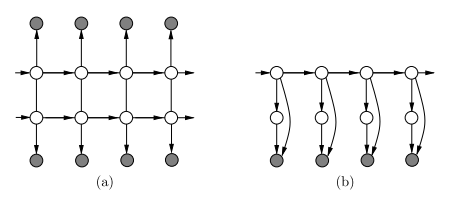
\includegraphics[width=.8\linewidth]{2-6.PNG}
    \caption{
        HMM 在语言和语音处理中的拓展。
        (a) 耦合 HMM。
        (b) 带有混合模型的 HMM。
    }\label{fig:2-6}
\end{figure}

另一类在语言处理中被广泛研究的模型叫“词袋(Bag-of-words)”模型,尤其在大规模文档语料建模中很常见。
词袋的意思是假设文档中单词的顺序不重要,亦即假设了单词位置的可交换性。
这些模型的目标通常是在语料库中找到潜在的“主题”,并利用这些主题对文档进行聚类或者分类。
词袋模型的一个实例是隐迪利克雷分配(Latent Dirichlet Allocation, LDA),在这个模型中,主题是定义在单词上的概率分布,文档是定义在主题上的概率分布。
特别地,如图 \ref{fig:2-7} 所示,语料库中的每篇文档都假设是通过采样一个带有超参数 $\alpha$ 的 Dirichlet 变量,然后根据这些 Dirichlet 概率反复选择一个主题,并从与所选主题相关的分布中选择一个单词来生成的 \footnote{这个模型将会在 3.3 小节中的例 3.5 进行详细讲解。}。

\begin{figure}[htbp]
    \centering
    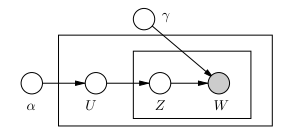
\includegraphics[width=.5\linewidth]{2-7.PNG}
    \caption{
        LDA 的图模型表示。
        变量 $U$ 遵从参数为 $\alpha$ 的 Dirichlet 分布,“主题”变量 $Z$ 遵从参数为 $U$ 的多项分布。
        “单词”变量 $W$ 同样是基于 $Z$ 的多项分布,$\gamma$ 指定与每个主题相关的单词概率。
        这些矩形称作盘子(Plates),在矩形内部的随机变量是保持条件独立性进行重复的。
    }\label{fig:2-7}
\end{figure}

\subsection{图像处理和空间统计}

几十年来,无向图模型或马尔可夫随机场在图像处理和更一般的空间统计中发挥了重要作用。
对于图像建模,最简单的马尔可夫随机场是在像素域,图像中的每个像素都与底层图中的一个节点相关联。
还有很多其他的结构化模型是建立在每个空间位置的特征向量上的,其中每个特征可以是一个线性多尺度滤波器(如小波)或者更复杂的非线性算子。

对于图像建模,一个最自然的图结构是 2D 网格,例如图 \ref{fig:2-8}(a) 中所示 4-最近邻网络。
通常选择相邻像素(或者更一般的特征)连边上的势函数来表示局部平滑条件。
图像处理的各种任务,包括去噪、分割和超分辨率等,都需要在这样的马尔可夫随机场上解决相应的推断问题。
然而对于大规模格点模型的精确推断是很难的,因此需要近似算法。
MCMC 方法被用得很多,但是对于很多应用来说计算量可能太大,速度不够快。
最近诸如和积算法与树重加权(Tree-Reweighted)最大积算法等消息传递算法已成为图像处理和计算机视觉问题的一种近似推断方法。

另一种策略是用一个更简单的——近似的——模型来代替格点模型,从而避开格点模型的难处。
例如多尺度 4 叉树,如图 \ref{fig:2-8}(b) 所示,就能用来近似格点模型。
这种多尺度模型的优点是允许利用高效的树算法来进行精确推断。
然而带来的问题是模型不完美,可能会导致图像重构中出现伪影。

\begin{figure}[htbp]
    \centering
    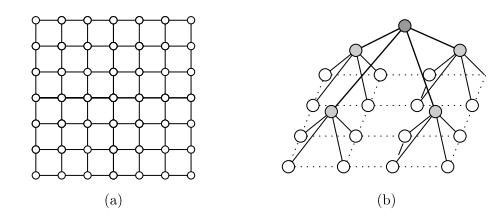
\includegraphics[width=.8\linewidth]{2-8.PNG}
    \caption{
        (a) 2D 的 4-近邻网格模型经常被用来做图像建模。
        (b) 多尺度的 4 叉树 2D 格点近似模型。
        原始格点(白色)对应的节点位于树的最小尺度上。
        树的中部和顶部尺度由辅助节点构成(灰色),引入辅助节点对精细尺度行为进行建模。
    }\label{fig:2-8}
\end{figure}

\subsection{纠错编码}

通信理论的核心问题是把信息以比特序列的形式从一点传送到另一点。
例如个人计算机在网络上的通信或者从卫星到地面的通信等。
如果通信信道是有噪声的,那么某些传输位可能被损坏。
为了对抗这种噪声,一种自然的策略是给传输的比特序列添加冗余,从而定义编码字。
原则上,这种编码策略允许在存在一些错误的情况下完美地解码通信。

现在使用的很多最好的编码,包括 Turbo 码和低密度奇偶校验码,都是基于图模型的。
图 \ref{fig:2-9}(a) 展示了一个非常小的奇偶校验码的因子图形式。
(图 \ref{fig:2-9}(b) 展示了更大的编码)。
在左边,6 个白色节点代表组成编码字 $x_i$(也就是长度为 6 的二元序列),而灰色节点代表与这些比特序列相关的噪声观测结果 $y_i$。
在右边,每个黑色方块节点代表一个因子 $\psi_{stu}$,表示三元组 $\{x_s, x_t, x_u\}$ 的奇偶性。
该奇偶关系在数学上表示为 $x_s \oplus x_t \oplus x_u \equiv z_{stu}$ 的模二算法,可以用如下形式的势函数表示为无向图模型:
$$\psi_{stu}(x_s, x_t, x_u) \coloneqq \begin{cases}
    1 & \text{如果} x_s \oplus x_t \oplus x_u = 1 \\
    0 & \text{其他}
\end{cases}$$
对于图 \ref{fig:2-9} 所示的编码,奇偶校验范围在三元组 $\{1, 3, 4\}$、$\{1, 3, 5\}$、$\{2, 4, 6\}$ 和 $\{2, 5, 6\}$ 的集合上。

解码问题需要根据噪声观测的向量 $y = (y_1, y_2, \dots, y_m)$ 来估计传输的是哪个编码字。
有了信道噪声模型的表示,这个解码问题可以归结为一个推断问题。
根据损失函数,最佳解码要么基于每个节点边际概率 $p_s(x_s = 1|y)$ 计算,要么直接计算最可能的编码字(即后验的众数)。
对于图 \ref{fig:2-9}(a) 的简单编码,通过联合树算法可以很容易实现最优解码。
然而在很多应用中人们感兴趣的是比特数很容易达到几千位的大规模编码。
这些编码下的图模型有着很大的树宽值,因此联合树算法不可行。
此外 MCMC 算法在该领域也还没有得到成功的应用。

\begin{figure}[htbp]
    \centering
    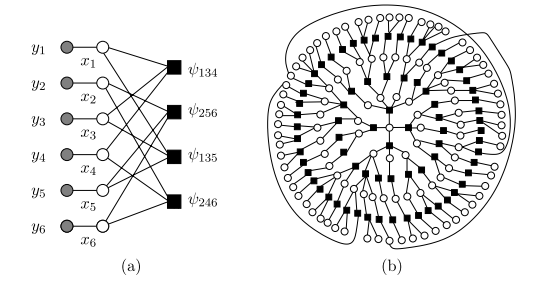
\includegraphics[width=.8\linewidth]{2-9.PNG}
    \caption{
        (a) 长度为 $m = 6$ 的奇偶校验码的一种因子图表示。
        在左边,圆形的白色节点代表定义编码的未观测比特位 $x_i$,而圆形的灰色节点代表从通道接收到的观测值 $y_i$。
        在右边,黑色方块代表相关的因子,或奇偶校验。
        这个特定的编码是 $(2, 3)$ 码,因为每个比特都与两个奇偶性变量相连,每个奇偶性关系涉及三个比特。
        (b) 具有“局部树状”结构的大型因子图。
        $m$ 个有界度节点上的因子图的随机构造具有典型长度 $\log{m}$ 的环,这种树状属性可以大大促进近似解码的和积算法的成功应用。
    }\label{fig:2-9}
\end{figure}

对于许多图编码,最成功的解码器是基于和积算法的,2.6 小节将对其进行详细讨论。
由于定义好的编码的图模型总是有环,和积算法不能保证计算出正确的边际,甚至有可能不能收敛。
尽管如此,这种近似解码算法对于大规模的编码来说还是有非常积极的意义。
和积算法在编码长度趋向于无穷的情况下是很容易理解的,可以使用鞅参数来证明收敛结果。
相较之下对于一般长度的编码就不那么好理解了。

\section{精确推断算法}

本节我们开始讲解图模型的基本精确推断算法。
在计算边际概率的时候,我们必须在一个或多个变量上对联合概率分布进行求和或者积分。
我们可以通过选择特定的变量顺序把这个计算过程表示为一个操作序列(可以利用 Fubini 定理)。
回想一下无论是有向还是无向图模型,联合概率都是变量子集的因子表达式。
因此我们可以充分利用分配律,调整求和或积分与乘积的顺序。
“精确推断”指的是组织计算顺序的问题,同时也需要对中间过程出现的新因子进行管理。
假设每个单独的求和或积分都计算得很精准,那么整个算法就会给出精确得数值结果。

为了得到单个变量 $X_s$ 的边际概率分布,只需要为其他变量指定一个顺序进行求和或积分消除即可。
对每个单独的变量重复整个过程就能得到完整的边缘集。
然而这种方法是低效的,因为它没有考虑有些中间项是可以在各个不同的边际计算过程中共用的。
和积算法和联合树算法本质上是基于共享中间项的动态规划算法。
算法涉及图结构上的“消息传递”操作,其中的消息就是指的这些可以共享的中间项。
如果算法收敛,我们就可以得到原图模型上所有团的边际概率。

有向图和无向图模型都涉及到联合概率分布的因子表达式,因此精确推断算法在本质上以相同的方式对它们进行处理。
实际上为了使得推断算法具有普适性,一般将有向图转换为无向图,并且统一在无向图的模式下进行处理。
我们可以看到有向图的因子分解 (2.1) 并不一定在团上定义,因为给定节点的父节点之间并不一定是连通的。
因此我们将一个有向图转换为一个无向的道德图(Moral Graph),其中每个子节点的父节点间都被连接,所有有向边都转换为无向边。
在这个道德图中,因子都是在团上进行定义的,因此任何有向分解 (2.1) 都是无向分解 (2.2) 的特例。
在这篇文章剩下的部分中,我们假设都已经进行了这种转换。

\subsection{树结构上的消息传递}

我们现在开始讨论用消息传递算法在树结构上进行精确推断。
我们在这里的讲解很简单,读者有兴趣的话可以参考相关的引文。
首先可以看到的是树 $T = (V, E(T))$ 上的团仅仅是单个的节点和边。
因此任何树形结构的图模型都能够进行以下分解:
\begin{equation}
    p(x_1, x_2, \dots, x_m) = \frac{1}{Z}\prod_{s \in V}\psi_s(x_s)\prod_{(s, t) \in E(T)}\psi_{st}(x_s, x_t)
\end{equation}
在这里我们稍微描述一下怎样对树结构的图上的任意节点使用和积算法计算边际概率
\begin{equation}
    \mu_s(x_s) \coloneqq \sum_{\{x'|x_s' = x_s\}}p(x_1', x_2', \dots, x_m')
\end{equation}
我们将重点讨论离散随机变量的情况,连续的情况原则上都可以利用积分替代求和得到。

和积算法:和积算法本质上是非串行动态规划的一种形式,它将确定性动态规划通常的串行形式推广到了任意的树形图。
动态规划(DP)的基本原则是分而治之:通过将一个大问题分解为一系列更简单的问题来进行解决。
在图模型中,树结构本身提供了一种对问题进行分解的自然方法。

对于任意节点 $s \in V$,考虑它的邻居集合
\begin{equation}
    N(s) \coloneqq \{u \in V| (s, u) \in E\}
\end{equation}
对于每个邻居节点 $u \in N(s)$,令 $T_u = (V_u, E_u)$ 为 $u$ 可以不用经过 $s$ 就能够到达的节点集(以及连接它们之间的边)所形成的子图。
树结构的一项关键属性就是这样的子图 $T_u$ 也仍然还是树结构,并且对于 $u \neq v$,$T_u$ 和 $T_v$ 的节点是没有重合的。
这样的话,每一个邻居节点 $u \in N(s)$ 都能被视为子树 $T_u$ 的根节点,如图 \ref{fig:2-10} 所示。

\begin{figure}[htbp]
    \centering
    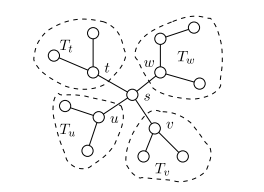
\includegraphics[width=.5\linewidth]{2-10.PNG}
    \caption{
        一棵以 $s$ 为根节点的树的分解。
        节点 $s$ 的每一个邻居节点 $u$ 都是一棵子树 $T_u$ 的根节点。
        在图中移除掉节点 $s$ 之后不同子树之间是不连通的。
    }\label{fig:2-10}
\end{figure}

对于每棵子树 $T_t$,我们定义与其节点变量相关的子向量 $x_{V_t} \coloneqq (x_u, u \in V_t)$。
现在考虑式 (2.4) 中 与子树 $T_t$ 的节点或边的相关的项的集合。
我们把这些项汇总到一起,写成下面的乘积形式:
\begin{equation}
    p(x_{V_t}; T_t) \propto \prod_{u \in V_t}\psi_u(x_u)\prod_{(u, v) \in E_t}\psi_{uv}(x_u, x_v)
\end{equation}
通过这种表示法,树的条件独立性允许将节点 $s$ 的边际计算分解为子问题的乘积,集合 $\{T_t, t \in N(s)\}$ 中每一棵子树都对应一个子问题,具体分解情形如下所示:
\begin{subequations}
\begin{align}
    \mu_s(x_s) &= \kappa\psi_s(x_s)\prod_{t \in N(s)}M_{ts}^*(x_s) \\
    M_{ts}^*(x_s) &\coloneqq \sum_{x_{V_t}'}\psi_{st}(x_s, x_t')p(x_{V_t}'; T_t)
\end{align}
\end{subequations}
上式中 $\kappa$ 为确保 $\mu_s$ 归一化的正数。
对于固定的 $x_s$,子问题定义的 $M_{ts}^*(x_s)$ 同样是一个树结构的求和,只不过这棵子树 $T_t$ 比原来的树 $T$ 小。
因此它也可以采用类似的方式进行递归分解。
这样,节点 $s$ 的边际就可以通过一系列递归更新来计算。

和积算法并不是将上述过程分别应用到每个节点,而是同时并行地计算所有节点地边际。
在每次迭代中,每个节点 $t$ 向它的邻居 $u \in N(t)$ 传递一条“消息”。
我们用 $M_{tu}(x_u)$ 来表示这个消息,它本质上是可能状态 $x_u \in \mathcal{X}_u$ 的一个函数(一个长度为 $|\mathcal{X}_u|$ 的离散随机向量)。
在整个图上一共有 $2|E|$ 条消息,每条边的每个方向上都有一条消息。
整个消息集合根据以下递归规则进行更新
\begin{equation}
    M_{ts}(x_s) \leftarrow \kappa\sum_{x_t'}\{\psi_{st}(x_s, x_t')\psi_t(x_t')\prod_{u \in N(t)/s}M_{ut}(x_t')\}
\end{equation}
其中 $\kappa > 0$ 是一个归一化常数。
可以证明,在树结构图上经过式 (2.9) 的有限次迭代将收敛到唯一的不动点 $M^* = \{M_{st}^*, M_{ts}^*, (s, t) \in E\}$。
所求得的不动点 $M_{ts}^*$ 与式 (2.8b) 中的子问题的解只差一个归一化常数。
由于不动点 $M^*$ 计算出了所有子问题的解,所有节点 $s \in V$ 的边际就可以轻松使用式 (2.8a) 计算出来。

最大积算法:将式 (2.9) 中的求和换成求最大值。
最大积算法可以用来求解树结构分布的众数问题。
在这个意义上可以把它看作是维特比算法从链式结构到树结构的推广。
更进一步地说,最大积算法将收敛到另一个与和积算法不同的唯一的不动点 $M^*$。
通过类比式 (2.7) 这个不动点可以用来计算图中任意节点的最大边际
\begin{equation}
    \nu_s(x_s) \coloneqq \max_{\{x'|x_s' = x_s\}}p(x_1', x_2', \dots, x_m')
\end{equation}
给定这些最大边际可以使用标准的回溯法(Back-tracking)来计算分布的众数 $\hat{x} \in arg\max_{x'}p(x_1', x_2', \dots, x_m')$。
更一般地,这种形式的更新适用于树结构图上的任意交换半环(Commutative Semirings)。
“和积”与“最大积”是这种代数结构的两个特例。

\subsection{联合树表示}

我们已经看到可以通过消息传递算法精确地解决树结构上的推断问题。
给定一个带环图,一种自然的想法是对它的节点进行聚类来形成一种团树(Clique Tree)结构——一种以 $G$ 上的最大团为节点而构成的无环图。
这么处理了之后就可以应用标准的树推断算法。
然而为了保证计算的正确性,团树还需要满足其他的限制条件。
特别地,由于给定顶点 $s \in V$ 可能出现在多个团中(如 $C_1$ 和 $C_2$),所以需要一种机制来保证变量 $x_s$ 在不同位置的一致性。
事实证明以下属性是保证这种一致性的充要条件:

\begin{tcolorbox}
\begin{defn}
    如果对于任意两个团节点 $C_1$ 和 $C_2$,在连接它们的唯一路径上的所有节点都包含交集 $C_1 \cap C_2$,则称这个团树具有运行交集性(Running Intersection Property)。
    具有运行交集性的团树称为联合树。
\end{defn}
\end{tcolorbox}

什么类型的图可以建立联合树?
图论中的一个重要结论建立了联合树与三角可分(Triangulation)之间的对应关系。
如果一个图中任意长度大于等于 4 的环中都有一根弦,也就是说环内有一条边连接一对不相邻的节点,我们就把这个图称为是三角可分的。
一个关键定理是图 $G$ 可以建立联合树当且仅当它是三角可分的。
这一结论为可用于对任意图进行精确推断的联合树算法奠定了基础:

\begin{enumerate}
    \item[(1)] 给定一个带环图 $G$,必要时通过添加边对其进行三角化处理。
    \item[(2)] 根据三角可分图 $\widetilde{G}$ 构建相应的联合树。
    \item[(3)] 在联合树上运行树推断算法。
\end{enumerate}

\begin{tcolorbox}
\begin{exam}[联合树]
    为了说明联合树的构建过程,考虑图 \ref{fig:2-11}(a) 中所示的 $3 \times 3$ 网格。
    第一步是建立一个三角可分图 $\widetilde{G}$,如图 \ref{fig:2-11}(b) 所示。
    注意如果节点 2 和节点 8 的附加边不存在的话,图不是三角可分的。
    如果没有这条边,4-环 $(2-4-8-6-2)$ 就会缺少一条弦。
    由于这条附加边的存在,联合树中出现了两个 4-团,如图 \ref{fig:2-11}(c) 所示。
\end{exam}
\end{tcolorbox}

\begin{figure}[htbp]
    \centering
    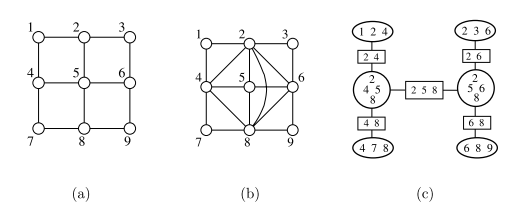
\includegraphics[width=.8\linewidth]{2-11.PNG}
    \caption{
        构建联合树的过程。
        (a) 原图是一个 $3 \times 3$ 的网格。
        (b) 原图的三角化版本。
        注意中间有两个 4-团。
        (c) 与 (b) 相对应的联合树,椭圆表示最大团,矩形表示分割子(Separator)。
    }\label{fig:2-11}
\end{figure}

原则上联合树算法的第三步中的推理可以在任意交换半环上执行(如我们之前在关于树算法的讨论中提到的)。
读者可以参考 Dawid 的作品,里面对最大积算法的联合树版本进行了广泛的讨论。
具体起见,我们在这里只讨论和积算法的联合树版本。
在联合树推断算法中通过在分割子——团结构之间的矩形(见图 \ref{fig:2-11})——上引入势函数而不仅仅只是在团结构上可以很优雅地表达基本的代数操作。
令 $\phi_C(\cdot)$ 代表在团结构 $C$ 上子向量 $x_C = (x_t, t \in C)$ 的势函数。
联合树上的团结构的势函数可以由原图的势函数获得。
分割子的势函数初始化为 1。
在此基础上可以给出联合树算法的基本消息传递步骤:
\begin{subequations}
\begin{align}
    \widetilde{\phi}_S(x_S) &\leftarrow \sum_{x_{B/S}}\phi_B(x_B) \\
    \phi_C(x_C) &\leftarrow \frac{\widetilde{\phi}_S(x_S)}{\phi_S(x_S)}\phi_C(x_C)
\end{align}
\end{subequations}
在连续的情况下求和可以用积分代替。
我们把这对操作称为“将消息从团 $B$ 传递到团 $C$”(如图 \ref{fig:2-12})。
可以验证一条消息如果从 $B$ 传递到 $C$ 再从 $C$ 传递到 $B$,结果彼此的团势是一致的,这意味着它们在节点集 $S$ 上是一致的。

\begin{figure}[htbp]
    \centering
    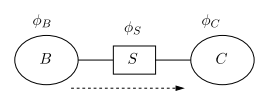
\includegraphics[width=.5\linewidth]{2-12.PNG}
    \caption{
        团 $B$ 和团 $C$ 之间通过分割子集 $S$ 的一次消息传递操作。
    }\label{fig:2-12}
\end{figure}

在联合树上经过一轮消息传递之后,可以看到整个联合树上团势与边际概率成正比。
也就是说,令 $\mu_C(x_C)$ 代表 $x_C$ 的边际概率,则有 $\mu_C(x_C) \propto \widetilde{\phi}_C(x_C)$。
这个性质可以通过对前面所介绍的和积算法的证明进行适当地推广得到(参见 Lauritzen 的作品)。
请注意,如果团势与边际概率是成比例的,那么每一对团结构之间满足局部的一致性显然是一个必要条件。
这就是运行交集性的意义所在,保证局部一致性蕴含全局一致性。

联合树算法有一个很重要的衍生结论,可以对分布 $p$ 表示成另外一种形式。
令 $\mathcal{C}$ 代表 $\widetilde{G}$ 中的最大团集合(也就是联合树中的节点),令 $\mathcal{S}$ 表示分割子的集合(也就是联合树中团结构之间的交集)。
要注意的是给定的分割子 $S$ 可能在联合树上出现很多次。
对于每个给定的分割子 $S \in \mathcal{S}$,设 $d(S)$ 表示其相邻的最大团的数目。
联合树框架使得分布 $p$ 可以按照下式进行因子分解
\begin{equation}
    p(x_1, x_2, \dots, x_m) = \frac{\prod_{C \in \mathcal{C}}\mu_C(x_C)}{\prod_{S \in \mathcal{S}}[\mu_S(x_S)]^{d(S)-1}}
\end{equation}
其中 $\mu_C$ 和 $\mu_S$ 分别代表团结构和分割子上的边际分布。
不同于因子分解式 (2.2),式 (2.12) 是直接以边际分布的形式来表达的,也不需要什么归一化常数(也就是说 $Z = 1$)。

\begin{tcolorbox}
\begin{exam}[马尔可夫链]
    考虑如下只包含三个变量的一个简单马尔可夫链 $p(x_1, x_2, x_3) = p(x_1)p(x_2|x_1)p(x_3|x_2)$。
    对应的图模型上的团包括 $\{1, 2\}$ 和 $\{2, 3\}$,之间的分割子为 $\{2\}$。
    很显然这个分布不能写成只包括团的边际的乘积。
    但是我们引入分割子之后就能写成下面这种边际形式:
    \[p(x_1, x_2, x_3) = \frac{p(x_1, x_2)p(x_2, x_3)}{p(x_2)}\]
    而且很容易验证这种边际的形式可以从式 (2.11) 导出,只需要设定 $\phi_{\{1, 2\}}(x_1, x_2) = p(x_1)p(x_2|x_1)$、$\phi_{\{2, 3\}}(x_2, x_3) = p(x_3|x_2)$。
\end{exam}
\end{tcolorbox}

为了给我们后续的内容做铺垫,考虑如下关于联合树表示的一种“反向”视角。
假设我们得到了一组关于联合树上团结构和分割子的函数 $\{\tau_C, C \in \mathcal{C}\}$ 与 $\{\tau_S, S \in \mathcal{S}\}$。
有哪些条件能够使得这些函数成为某种分布的有效边际?
假设这些函数在以下意义上是局部一致的:
\begin{subequations}
\begin{align}
    \forall S \in \mathcal{S}, &\sum_{x_S'}\tau_S(x_S') = 1 \\
    \forall C \in \mathcal{C}, S \subseteq C, &\sum_{\{x_C'|x_S' = x_S\}}\tau_C(x_C') = \tau_S(x_S)
\end{align}
\end{subequations}
上述联合树理论的本质是,这种局部一致性就是保证这些函数是某种分布的有效边际的充要条件。
为便于以后参考,我们将此结论做如下声明:
\begin{tcolorbox}
\begin{prop}
    函数组 $\{\tau_C, C \in \mathcal{C}\}$ 与 $\{\tau_S, S \in \mathcal{S}\}$ 可以作为联合树上团结构与分割子的边际分布当且仅当对于所有分割子 $S \in \mathcal{S}$ 都有归一化式 (2.13a) 从成立,且对于所有团结构 $C \in \mathcal{C}$ 都有边际化式 (2.13b) 成立。
    此外,所有满足这种局部一致性的函数都是由式 (2.12) 所定义的概率分布的边际。
\end{prop}
\end{tcolorbox}
这种联合树的表示形式将在我们后续的内容中发挥很大的作用。

最后我们讨论一下关于联合树算法计算复杂度的问题。
式 (2.11) 表明计算代价将随着联合树中最大团的规模呈指数增长。
显然人们感兴趣的就是控制团的规模。
图上所有潜在的三角形上的最大团的规模是一个重要的图论量,称为图的树宽\footnote{更准确地说,树宽是最大团的规模减一}。
因此,联合树算法的复杂度在树宽上呈指数级。

对于某些类型的图,例如链结构和树结构,树宽较小,联合树算法为推断问题提供了有效的解决方案。
很多著名的图模型架构都是如此,从中可以得到联合树算法的多种经典递归变体,包括计算遗传学中的剪枝和削皮算法,隐马尔可夫模型的前后向算法,状态空间模型的卡尔曼滤波算法等。
另一方面,也有许多图模型的树宽相当大,包括 2.4 小节中谈到的几个例子。
为了解决这种图模型必须放弃联合树框架,转而去寻找近似推断算法。

\section{近似推断的消息传递算法}

本书剩余部分的内容是提出一种近似计算边际分布和似然以及整数规划的变分方法理论框架。
这样做需要凸分析和指数族的数学背景知识,我们将在第三章中提供。
然而从历史上看,许多算法是在没有这些背景的情况下发展起来的,它们依赖的是物理直觉或者是对精确或近似蒙特卡洛算法的类比。
在本节中我们将对两种变分推断算法的这种特性进行高层次的描述,以突出它们的简单和直观性质。

我们考虑的第一个变分算法是应用于带环图的和积消息传递,被称为“循环的(Loopy)”和积算法或者信念传播算法(Belief propagation)。
回想一下,和积算法是树结构的精确推断算法,然而但从算法的角度上来说,当然也可以尝试将它应用到带环图上。
更具体地说,消息更新式 (2.9) 可以在给定的节点上运行,忽略环的存在就行。
直观上来讲,如果图比较稀疏或者存在某种特殊的对称性,这样的算法可能可行,因为在环上传播的影响会比较小。
正如 2.4 小节中讨论的,该算法实际上已经成功地获得了很多的应用。
此外,最大积算法的一种类似形式也可以用来计算带环图上的近似众数。

第二种变分算法就是所谓的朴素平均场算法(Naive Mean Field)。
我们将会描述该算法在 Ising 模型中的应用,这是一个包含二元随机向量 $X \in \{0, 1\}^m$ 的无向图模型或者马尔可夫随机场,其中相邻节点对有一个耦合权重 $\theta_{st}$,每一个节点还有一个观测权重 $\theta_s$。
(关于该模型的详细描述参见 3.3 解的例 3.1。)
为了给朴素平均场提供一些直观认识,我们首先在这个特殊的模型上描述吉布斯采样(Gibbs Sampler),这是一种特殊类型的 MCMC 算法。
吉布斯采样的基本步骤是随机选择一个节点 $s \in V$,然后在邻居状态固定的情况下,根据条件概率更新相关随机变量的状态。
更准确地说,令 $N(s)$ 表示节点 $s \in V$ 的邻居,令 $X_{N(s)}^{(n)}$ 代表节点 $s$ 的邻居在第 $n$ 次迭代时的状态,则节点 $s$ 的状态更新如下
\begin{equation}
    X_s^{(n+1)} = \begin{cases}
        1 & \text{如果} U \leq \{1 + \exp{[-(\theta_s + \sum_{t \in N(s)}\theta_{st}X_t^{(n)})]}\}^{-1} \\
        0 & \text{其他}
    \end{cases}
\end{equation}
其中 $U$ 为采样自均匀分布 $\mathcal{U}[0, 1]$ 的一个样本。

在稠密图中,这样的邻居集合 $N(s)$ 的基数可能很大,我们可以尝试使用大数定律或者其他计算方式来估计 $\sum_{t \in N(s)}\theta_{st}X_t^{(n)}$。
就这个求和的稠密程度而言,用期望代替样本值可能比较有效。
也就是说,令 $\mu_s$ 代表每个节点 $s \in V$ 边际概率 $\mathbb{P}[X_s = 1]$ 的一个估计值,我们可以考虑式 (2.14) 的一个平均形式:
\begin{equation}
    \mu_s \leftarrow \{1 + \exp{[-(\theta_s + \sum_{t \in N(s)}\theta_{st}\mu_t)]}\}^{-1}
\end{equation}
因此与其依赖其邻居状态的条件概率更新随机变量 $X_s$,不如确定性地更新一个参数 $\mu_s$,它也依赖于其邻居的相应参数。
式 (2.15) 定义了 Ising 模型的朴素平均场算法。
与和积算法一样,平均场算法也可以看作是一种消息传递算法,式 (2.15) 右边表示到达节点 $s$ 的“消息”。

乍一看这种消息传递算法似乎还有些问题。
算法会导致不动点吗?
算法会收敛吗?
本书剩下的内容就是对这些问题进行讲解。
最终我们将看到一大类消息传递算法,包括平均场算法、和积算法、最大积算法,以及这些方法的各种拓展,都可以被理解为变分问题的精确或者近似的版本。
指数族和凸分析是下一章的主题,它们提供了一种统一的框架来发展这些变分原理。



\chapter{指数族表示的图模型}

指数族分布已经被各种文献广泛研究,本章将讲解能被作为指数族对待的一系列图模型。
采用指数族的观点可以阐述推断算法和凸分析理论之间的一些基本联系。
更具体地说,正如我们将看到的,图模型中各类推断问题可以通过平均参数和标准参数之间的映射来理解。

\section{指数族与最大熵原理}

导出图模型指数族表示的一个基本出发点是最大熵原理。
我们首先从简单的标量随机变量 $X$ 入手,探索一下有哪些可供后来借鉴的启示。
假设有 $n$ 个独立同分布(i.i.d.)的观测值 $X^1, \dots, X^n$,我们可以计算特定函数的经验期望值——也就是
\begin{equation}
    \hat{\mu}_{\alpha} \coloneqq \frac{1}{n}\sum_{i = 1}^n\phi_{\alpha}(X^i), \quad \forall \alpha \in \mathcal{I}
\end{equation}
其中在某个集合 $\mathcal{I}$ 中的每个 $\alpha$ 都可以索引到一个函数 $\phi_{\alpha}: \mathcal{X} \rightarrow \mathbb{R}$。
例如我们设 $\phi_1(x) = x$,$\phi_2(x) = x^2$,则式 (3.1) 对应随机变量 $X$ 的一阶和二阶矩的经验估计值。
基于这个 $|\mathcal{I}|$-维的经验估计向量 $\hat{\mu} = (\hat{\mu}_{\alpha}, \alpha \in \mathcal{I})$,我们的目标是去推断随机变量 $X$ 的全概率分布。
特别地,我们将概率分布表示为关于某个测度 $\nu$ 的绝对连续的密度 $p$。
这个基本测度 $\nu$ 可以是 $\{0, 1, \dots, r-1\}$ 的计数测度,此时 $p$ 对应一个概率质量函数,或者对于连续随机向量,基本测度 $\nu$ 可以是 $\mathbb{R}$ 上的勒贝格测度。

对于一个给定的分布 $p$,假设期望值 $\mathbb{E}[\phi_{\alpha}(X)] \coloneqq \int_{\mathcal{X}}\phi_{\alpha}(x)p(x)\nu(dx)$,$\alpha \in \mathcal{I}$。
如果满足条件
$$\mathbb{E}_p[\phi_{\alpha}(X)] = \hat{\mu}_{\alpha}, \quad \forall \alpha \in  \mathcal{I}$$
我们称分布 $p$ 和数据一致。
换句话说就是在分布 $p$ 下的期望 $\mathbb{E}_p[\phi_{\alpha}(X)]$ 与经验分布一致。
一般来说有很多分布 $p$ 与数据一致,因此需要一个原则来决定选择其中一个来作为 $X$ 最佳的全概率分布。

我们引入香农熵(Shannon Entropy)
\begin{equation}
    H(p) \coloneqq -\int_{\mathcal{X}} (\log{p(x)})p(x)\nu(dx)
\end{equation}
最大熵原理是指从与数据一致的分布中选择香农熵最大的分布 $p^*$。
严格地说,令 $\mathcal{P}$ 代表随机变量 $X$ 所有可能分布的集合,最大熵解 $p^*$ 由下面的约束优化问题给出:
\begin{equation}
    p^* \coloneqq arg\max_{p \in \mathcal{P}}H(p) \quad \text{subject to } \mathbb{E}_p[\phi_{\alpha}(X)] = \hat{\mu}_{\alpha}, \quad \forall \alpha \in \mathcal{I}
\end{equation}
对最大熵原理的一种解释是在保持数据一致性的条件下选择具有最大不确定性(由熵函数 (3.2) 度量)的分布。
如果问题 (3.3) 有解,在连续情况下可以使用变分法,在离散情况下可以直接计算,最优解 $p^*$ 具有这种形式
\begin{equation}
    p_{\theta}(x) \propto \exp{\{\sum_{\alpha \in \mathcal{I}}\theta_{\alpha}\phi_{\alpha}(x)\}}
\end{equation}
其中 $\theta \in \mathbb{R}^d$ 表示指数族形式下的一组参数。
从最大熵的角度来看,参数 $\theta$ 有一个非常具体的解释,那就是和经验量 $\hat{\mu}$ 约束相关的一组拉格朗日乘子。
下面的章节中我们将对这种联系进行更为深入的探索。

\section{指数族的基础内容}

经过上面那个例子的启发之后,我们来建立指数族的标准框架。
更准确地说,指数族是建立在基本测度 $\nu$ 之上的一些参数化的密度函数。

给定取值空间为 $\mathcal{X}^m = \otimes_{s = 1}^m\mathcal{X}_s$ 的一个随机向量 $(X_1, X_2, \dots, X_m)$,令 $\phi = (\phi_{\alpha}, \alpha \in \mathcal{I})$ 为一系列函数 $\phi_{\alpha}: \mathcal{X}^m \rightarrow \mathbb{R}$ 的集合,这些函数也就是势函数(Potential functions)或者充分统计量(Sufficient Statistics)。
$\mathcal{I}$ 是一个包含 $d = |\mathcal{I}|$ 个元素的索引集,因此 $\phi$ 也可以看作是将 $\mathcal{X}^m$ 映射到 $\mathbb{R}^d$ 的向量值函数。
对于一个给定的充分统计量向量 $\phi$,令 $\theta = (\theta_{\alpha}, \alpha \in \mathcal{I})$ 代表相关的一组量,这组量被称为标准参数(Canonical Parameters)或者指数参数。
对于每个向量 $x \in \mathcal{X}^m$,我们使用 $\langle \theta, \phi(x) \rangle$ 代表 $\mathbb{R}^d$ 空间中 $\theta$ 与 $\phi(x)$ 两个向量的欧几里得内积。

采用这些符号可以把与 $\phi$ 相关的指数族表示为以下带参密度函数形式
\begin{equation}
    p_{\theta}(x_1, x_2, \dots, x_m) = \exp{\{\langle \theta, \phi(x) \rangle - A(\theta)\}}
\end{equation}
相应的测度为 $\nu$ \footnote{对于任意的可测集 $S$,我们有 $\mathbb{P}[X \in S] = \int_Sp_{\theta}(x)\nu(dx)$。}。
其中 $A$ 被称为对数配分函数(Log Partition Function)或者累积函数(Cumulant Function),由以下积分定义
\begin{equation}
    A(\theta) = \log{\int_{\mathcal{X}^m}\exp{\langle \theta, \phi(x) \rangle}\nu(dx)}
\end{equation}
假设积分存在,整个定义保证了 $p_{\theta}$ 是归一化的($\int_{\mathcal{X}^m}p_{\theta}\nu(dx) = 1$)。
对于给定的一组势函数 $\phi$,每一个参数向量 $\theta$ 对应族内的一个特定分布 $p_{\theta}$。
我们感兴趣的标准参数 $\theta$ 属于下面这个集合
\begin{equation}
    \Omega \coloneqq \{\theta \in \mathbb{R}^d| A(\theta) < +\infty\}
\end{equation}
我们很快就会看到 $A$ 是 $\theta$ 的一个凸函数,这也表示 $\Omega$ 必须是一个凸集。
对数配分函数 $A$ 在本文中有着很重要的作用。

以下概念在接下来的内容里面很重要:

正则族(Regular Families):$\Omega$ 为开集的指数族称为正则族。
尽管确实存在 $\Omega$ 为闭集的指数族(参见 Brown 的作品),但是我们在这里主要把注意力放在正则族上。

最小性(Minimal):有一类典型的指数族,对于它们的充分统计量 $\phi = (\phi_{\alpha}, \alpha \in \mathcal{I})$,不存在非零向量 $a \in \mathbb{R}^d$ 使得线性组合
$$\langle a, \phi(x) \rangle = \sum_{\alpha \in \mathcal{I}}a_{\alpha}\phi_{\alpha}(x)$$
为一个常数(在 $\nu$ 测度下几乎处处满足)。
这个条件导致了一个所谓的最小表示(Minimal Representation),其中每个分布由唯一的参数向量 $\theta$ 决定。

过完备性(Overcomplete):有时候不使用最小表示,而是采用非最小或者过完备表示(Overcomplete Representation)会很方便,也就是存在线性组合 $\langle a, \phi(x) \rangle$ 等于一个常数。
在这种情况下,参数向量 $\theta$ 的整个仿射子集都可以代表相同的一个分布。
读者可能会怀疑过完备表示的效果。
的确,从统计的角度来看这是不可取的,因为丢失了参数向量 $\theta$ 的可识别性。
然而这种过完备的概念在理解和积算法及其变体的时候将会很有帮助(参见第四章)。

表 \ref{tab:3-1} 提供了一些常见的标量指数族的例子。
注意这些族都是正则族($\Omega$ 是开集)和最小族(充分统计量 $\phi$ 线性无关)。

\begin{sidewaystable}[htbp]
\caption{
    几类常见的标量随机变量的指数族
}\label{tab:3-1}
\centering
\begin{threeparttable}
\begin{tabular}{lccccc}
    \hline
    Family & $\mathcal{X}$ & \tabincell{c}{$\nu$ \\ $h(\cdot)$} & $\langle \theta, \phi(x) \rangle$ & $A(\theta)$ & $\Omega$ \\
    \hline
    Bernoulli & $\{0, 1\}$ & Counting & $\theta x$ & $\log{[1+\exp{(\theta)}]}$ & $\mathbb{R}$ \\
    Gaussian & $\mathbb{R}$ & Lebesgue & $\theta x$ & $\frac{1}{2}\theta^2$ & $\mathbb{R}$ \\
    Location family & & $h(x) = \frac{\exp{(-x^2/2)}}{\sqrt{2\pi}}$ & & & \\
    Gaussian & $\mathbb{R}$ & Lebesgue & $\theta_1x + \theta_2x^2$ & $-\frac{\theta_1^2}{4\theta_2^2} - \frac{1}{2}\log{(-2\theta_2)}$ & $\{(\theta_1, \theta_2) \in \mathbb{R}^2| \theta_2 < 0\}$ \\
    Location-scale & & $h(x) = \frac{1}{\sqrt{2\pi}}$ & & & \\
    Exponential & $(0, +\infty)$ & Lebesgue & $\theta x$ & $-\log{(-\theta)}$ & $(-\infty, 0)$ \\
    Poison & $\{0, 1, 2, \dots\}$ & \tabincell{c}{Counting \\ $h(x) = 1/x!$} & $\theta x$ & $\exp{(\theta)}$ & $\mathbb{R}$ \\
    Beta & $(0, 1)$ & Lebesgue & \tabincell{c}{$\theta_1\log{x}$ \\ $+\theta_2\log{(1-x)}$} & \tabincell{c}{$\sum_{i = 1}^2\log{\Gamma(\theta_i+1)}$ \\ $-\log{\Gamma(\sum_{i = 1}^2(\theta_i+1))}$} & \\
    \hline
\end{tabular}
\begin{tablenotes}
    \item 注意:以上示例的基本测度 $\nu$ 要么是计数测度要么是勒贝格测度,与空间 $\mathcal{X}$ 严格相符,在某些例子中由因子 $h(\cdot)$ 进行调整。
        所有示例均为最小族和正则族。
\end{tablenotes}
\end{threeparttable}
\end{sidewaystable}

\section{指数形式的图模型示例}

表 \ref{tab:3-1} 中的标量示例可以作为更复杂的具有图结构的指数族的构建模块使用。
前面我们使用函数的乘积来描述图模型,如式 (2.1) 与 (2.2),这些乘积在指数族的形式里变成了求和。
在这里我们讨论一些常见的指数族形式的图模型示例。
熟悉这些例子的读者可以直接跳到 3.4 小节,在那里我们将继续对指数族进行一般性的讨论。

\begin{tcolorbox}
\begin{exam}[伊辛模型]

伊辛模型(Ising Model)来自于统计物理,是一个典型的指数族形式图模型。
考虑图 $G = (V, E)$,假设与节点 $s \in V$ 相关的随机变量 $X_s$ 是 Bernoulli 的,例如取“自旋”值 $\{-1, +1\}$。
在统计物理学的背景下,这些值可能代表磁场中磁极的方向,或者气体中粒子的存在或不存在。
伊辛模型及其变体也被用于图像处理和空间统计,其中 $X_s$ 可能对应于黑白图像的像素值,还可以被用于社交网络建模,例如政客的投票模式。

仅当图上节点 $s$ 和 $t$ 被边相连的时候,随机向量 $X$ 的组分 $X_s$ 和 $X_t$ 才会有直接交互。
这种设定可以导出如下密度的指数族
\begin{equation}
    p_{\theta}(x) = \exp{\{\sum_{s \in V}\theta_sx_s + \sum_{(s, t) \in E}\theta_{st}x_sx_t - A(\theta)\}}
\end{equation}
其中基本测度 $\nu$ 为被限定在 $\{0, 1\}^m$ 上的计数测度\footnote{更准确地说,对于每个单元素集合 $\{x\}$,如果 $x \in \{0, 1\}^m$,则 $\nu(\{x\}) = 1$,否则 $\nu(\{x\}) = 0$,而且可以由次可加性(Sub-additivity)扩展到任意集合。}。
这里 $\theta_{st} \in \mathbb{R}$ 代表边的强度,$\theta_s \in \mathbb{R}$ 代表节点 $s$ 的势,在统计物理中模拟一个“外场”,或者在空间统计中模拟一个有噪声的观测值。
严格地说,式 (3.8) 定义的密度族比经典的伊辛模型更为一般,经典伊辛模型的 $\theta_{st}$ 对所有边都相等。

作为一个指数族,伊辛模型的索引集 $\mathcal{I}$ 为 $V \cup E$,族的维度为 $d = m + |E|$。
对数配分函数由下面的求和给出
\begin{equation}
    A(\theta) = \log{\sum_{x \in \{0, 1\}^m}\exp{\{\sum_{s \in V}\theta_sx_s + \sum_{(s, t) \in E}\theta_{st}x_sx_t\}}}
\end{equation}
由于这个求和对于所有的 $\theta \in \mathbb{R}^d$ 都是有限的,因此 $\Omega$ 为整个空间 $\mathbb{R}^d$,为正则族。
此外这是一种最小表示,因为对于势函数来说不存在结果为常数的线性组合。

标准的伊辛模型可以从许多不同的方面进行推广。
尽管式 (3.8) 只包含两两相互作用,但随机变量之间的高阶交互作用也可以包括进来。
例如,为了包含 3-团 $\{s, t, u\}$ 的耦合作用,我们可以在式 (3.8) 中再添加一项 $x_sx_tx_u$,相关的标准参数设为 $\theta_{stu}$。
更一般地,对于 $k$-团之间的耦合,我们可以添加一直到 $k$ 阶的项,统计物理学中的 $k$-自旋模型就是这么来的。
当阶数取到最高 $k = m$ 时,图模型可以表示二元随机向量 $X \in \{0, 1\}^m$ 的任意分布。

\end{exam}
\end{tcolorbox}

\begin{tcolorbox}
\begin{exam}[度量标记和波茨模型]

我们考虑伊辛模型的另一种一般化版本:假设每个节点 $s \in V$ 对应的随机变量 $X_s$ 从离散空间 $\mathcal{X} \coloneqq \{0, 1, \dots, r-1\}$ 中取值($r > 2$)。
状态 $j \in  \mathcal{X}$ 可以看作一个标签,例如图像分割问题中定义的隶属类别。
每一对节点 $s \in V$ 和状态 $j \in \mathcal{X}$ 都可以派生出一个充分统计量
\begin{equation}
    \mathbb{I}_{s;j}(x_s) = \begin{cases}
        1 & \text{如果} x_s = j \\
        0 & \text{其他}
    \end{cases}
\end{equation}
相关的标准参数向量为 $\theta_s = \{\theta_{s;j}, j = 0, \dots, r-1\}$。
此外,每条边 $(s, t)$ 和每对状态值 $(j, k) \in \mathcal{X} \times \mathcal{X}$ 也可以定义一个充分统计量
\begin{equation}
    \mathbb{I}_{st;jk}(x_s, x_t) = \begin{cases}
        1 & \text{如果} x_s = j \text{且} x_t = k \\
        0 & \text{其他}
    \end{cases}
\end{equation}
相关的标准参数为 $\theta_{st;jk} \in \mathbb{R}$。
以上定义的充分统计量可以构成一个维数为 $d = r|V| + r^2|E|$ 的指数族。
与伊辛模型相似,对数配分函数处处有限,因此这个指数族是正则的。
然而与伊辛模型不同的是,这个指数族是过完备的:充分统计量之间有很多种线性相关关系存在,例如对于任意节点 $x_s \in V$ 都有 $\sum_{j \in \mathcal{X}}\mathbb{I}_{s;j}(x_s) = 1$。

度量标记问题(Metric Labeling)是这个模型的一个特例,它引入了一个度量 $\rho: \mathcal{X} \times \mathcal{X} \rightarrow [0, \infty)$ 来确定参数,即对所有 $(j, k) \in \mathcal{X} \times \mathcal{X}$,都有 $\theta_{st;jk} = -\rho(j, k)$。
因此标准参数满足 $\forall k \in \mathcal{X}: \theta_{st;kk} = 0$,$\forall j \neq k: \theta_{st;jk} < 0$,以及逆三角不等式($\forall (j, k, l): \theta_{st;jl} \geq \theta_{st;jk} + \theta_{st;kl}$)。
这个模型的另一个特例是来自统计物理的波茨模型(Potts Model),波茨模型中对于任意的 $k \in \mathcal{X}$ 都有 $\theta_{st;kk} = \alpha$,对于任意的 $j \neq k$ 都有 $\theta_{st;jk} = \beta$。

\end{exam}
\end{tcolorbox}

接下来我们讨论一类非常重要的在连续随机变量上构建的图模型:

\begin{tcolorbox}
\begin{exam}[高斯 MRF]

给定一个无向图 $G$ 和节点集 $V = \{1, \dots, m\}$,高斯马尔可夫随机场由满足 $G$ 上马尔可夫性(参见 2.2 小节)的多元高斯随机向量 $(X_1, \dots, X_m)$ 构成。
它可以用充分统计量 $(x_s, x_s^2, s \in V; x_sx_t, (s, t) \in E)$ 表示为指数族形式。
我们定义一个 $m$ 维向量 $\theta$ 作为充分统计量 $x = (x_1, \dots, x_m)$ 的相关参数,定义一个对称矩阵 $\Theta \in \mathbb{R}^{m \times m}$ 作为矩阵 $xx^T$ 的相关参数。
根据 Hammersley-Clifford 定理,矩阵 $\Theta$ 为逆协方差阵或精度矩阵的负值,它的特点是如果 $(s, t) \notin E$,则 $\Theta_{st} = 0$,如图 \ref{fig:3-1} 所示。
最终所得的指数族的维数为 $d = 2m + |E|$。

在这种设定下,多元高斯可以表达为如下指数族形式:
\begin{equation}
    p_{\theta}(x) = \exp{\{\langle \theta, x \rangle + \frac{1}{2}\langle \langle \Theta, xx^T \rangle \rangle - A(\theta, \Theta)\}}
\end{equation}
其中 $\langle \theta, x \rangle \coloneqq \sum_{i = 1}^m\theta_ix_i$ 为 $\mathbb{R}^m$ 上的欧几里得内积,此外
\begin{equation}
    \langle \langle \Theta, xx^T \rangle \rangle \coloneqq \text{trace}(\Theta xx^T) = \sum_{i = 1}^m\sum_{j = 1}^m\Theta_{ij}x_ix_j
\end{equation}
为对称阵上的 Frobenius 内积。
仅当 $\Theta \prec 0$ 的时候积分定义的 $A(\theta, \Theta)$ 才是有限的,因此
\begin{equation}
    \Omega = \{(\theta, \Theta) \in \mathbb{R}^m \times \mathbb{R}^{m \times m}| \Theta \prec 0, \Theta = \Theta^T\}
\end{equation}

\end{exam}
\end{tcolorbox}

\begin{figure}[htbp]
    \centering
    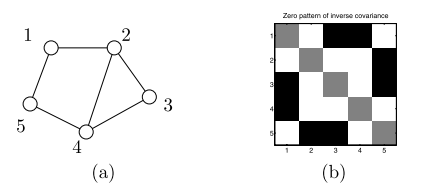
\includegraphics[width=.8\linewidth]{3-1.PNG}
    \caption{
        (a) 5 个节点的无向图模型。
        (b) 对于一个高斯马尔可夫随机场来说,它的逆协方差阵或者精度矩阵的零模式反映了图结构:对于任何一对 $i \neq j$,如果 $(i, j) \notin E$,那么 $\Theta_{ij} = 0$。
    }\label{fig:3-1}
\end{figure}

图模型并不局限于每个节点上的随机变量都属于同一指数族的情况。
更一般地,我们可以考虑指数族成员的异质组合,如下面的例子所示。

\begin{tcolorbox}
\begin{exam}[混合模型]

如图 \ref{fig:3-2}(a) 所示,一个标量混合模型的图表示十分简单。
具体说来,在一个有限混合高斯模型中,令 $X_s$ 代表一个多元变量,取值为 $\{0, 1, \dots, r-1\}$。
$X_s$ 所起的作用是对混合成分进行选择,因此我们一共有 $r$ 个成分。
和例 3.2 中描述的波茨模型一样,这个随机变量的分布是以 $\{\mathbb{I}_j[x_s], j = 0, \dots, r-1\}$ 为充分统计量,以 $\{\alpha_{s;0}, \dots, \alpha_{s;r-1}\}$ 为标准参数的指数族。

在混合模型中,给定 $X_s = j$,令 $Y_s$ 代表均值和方差为 $(\mu_j, \sigma_j^2)$ 的条件高斯。
每一个这样的条件分布都可以被写成是充分统计量为 $\{y_s, y_s^2\}$,标准参数为 $(\gamma_{s;j}, \gamma_{s;j}') \coloneqq (\frac{\mu_j}{\sigma_j^2}, -\frac{1}{2\sigma_j^2})$ 的指数族形式。
总之,我们可以得到整个模型的指数族形式,它的标准参数为
$$\theta_s \coloneqq (\underbrace{\alpha_{s;0}, \dots, \alpha_{s;r-1}}_{\alpha_s}, \underbrace{\gamma_{s;0}, \dots, \gamma_{s;r-1}}_{\gamma_s}, \underbrace{\gamma_{s;0}', \dots, \gamma_{s;r-1}'}_{\gamma_s'})$$
它的密度函数为
\begin{align}
    p_{\theta_s}(y_s, x_s) &= p_{\alpha}(x_s)p_{\gamma_s}(y_s|x_s)  \nonumber \\
    &\propto \exp{\{\sum_{j = 0}^{r-1}\alpha_{s;j}\mathbb{I}_j(x_s) + \sum_{j = 0}^{r-1}\mathbb{I}_j(x_s)[\gamma_{s;j}y_s + \gamma_{s;j}'y_s^2]\}}
\end{align}

$(X_s, Y_s)$ 为描述多元数据 $((X_1, Y_1), (X_2, Y_2), \dots, (X_m, Y_m))$ 的基本模块,可以用它来构建更加复杂的模型。
例如可以假设多元向量 $X = (X_1, \dots, X_m)$ 可以在某个基本图 $G = (V, E)$ 上构成马尔可夫随机场(参见例 3.2 中的波茨模型),变量 $Y_s$ 在给定 $\{X = x\}$ 的情况下条件独立。
根据这些可以导出一个参数为 $\theta = (\alpha, \gamma)$ 的指数族 $p_{\theta}(y, x)$,其密度为
\begin{equation}
    p_{\alpha}(x)p_{\gamma}(y|x) \propto \exp{\{\sum_{s \in V}\alpha_s(x_s) + \sum_{(s, t) \in E}\alpha_{st}(x_s, x_t)\}\prod_{s \in V}p_{\gamma_s}(y_s|x_s)}
\end{equation}
其中 $p_{\alpha}(x)$ 为波茨型(Potts-type)分布,$p_{\gamma}(y|x)$ 为局部条件分布。
$\alpha_s(x_s)$ 为 $\sum_{j = 0}^{r-1}\alpha_{s;j}\mathbb{I}_j(x_s)$ 的简写,$\alpha_{st}(x_s, x_t)$ 与此类似;非简写形式参见例 3.2。

\end{exam}
\end{tcolorbox}

\begin{figure}[htbp]
    \centering
    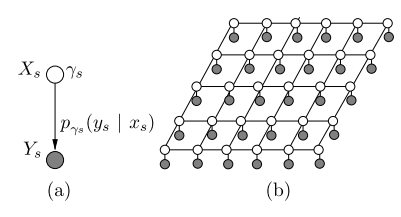
\includegraphics[width=.8\linewidth]{3-2.PNG}
    \caption{
        (a) 有限混合高斯模型的图表示:$X_s$ 为混合成分的多元标签,$Y_s$ 在给定 $X_s = j$ 的条件下是一个条件高斯量,$p_{\gamma_s}(y_s|x_s)$ 是以指数形式表示的高斯密度。
        (b) 耦合混合高斯图模型,向量 $X = (X_1, \dots, X_m)$ 是一个无向图上的马尔可夫随机场,$(Y_1, \dots, Y_m)$ 中的元素在给定 $X$ 时是条件独立的。
    }\label{fig:3-2}
\end{figure}

以上描述的混合模型存在两个层级,下面的例子存在三个层级:

\begin{tcolorbox}
\begin{exam}[隐迪利克雷分配]

隐迪利克雷分配(Latent Dirichlet Allocation,LDA)是一个典型的层次贝叶斯模型,用来捕获文档语料中词之间的统计依赖性。
模型涉及三种不同类型的随机变量:“文档(Documents)” $U$、“主题(Topics)” $Z$、“单词(Words)” $W$。
单词是分布在某个词汇表上的多元随机变量。
主题也是多元随机变量。
主题变量的每个值都与单词上的一个分布相关。
每篇文档可以看作是主题上的一个分布。
最终整个语料可以看作是文档上的一个分布。
在 LDA 模型中,语料对应的分布为迪利克雷分布。

更正式地说,单词 $W$ 取自一个多项分布,$\mathbb{P}(W = j|Z = i; \gamma) = \exp(\gamma_{ij}), \quad j = 0, 1, \dots, k-1$,其中 $\gamma_{ij}$ 代表第 $i$ 个主题下第 $j$ 个词出现的概率。
这个条件分布可以采用指示函数表达为指数族的形式:
\begin{equation}
    p_{\gamma}(w|z) \propto \exp(\sum_{i = 0}^{r-1}\sum_{j = 0}^{k-1}\gamma_{ij}\mathbb{I}_i(z)\mathbb{I}_j(w))
\end{equation}
其中 $\mathbb{I}_i(z)$ 为事件 $\{Z = i\}$ 的 $\{0, 1\}$ 指示值,$\mathbb{I}_j(w)$ 于此类似。
在层次结构的下一层(见图 \ref{fig:3-3}),主题变量 $Z$ 也遵循多项分布,其参数由迪利克雷变量确定如下:
\begin{equation}
    p(z|u) \propto \exp\{\sum_{i = 0}^{r-1}\mathbb{I}_i[z]\log u_i\}
\end{equation}
最后在层次结构的顶层,迪利克雷变量 $U$ 具有勒贝格测度下的密度形式 $p_{\alpha}(u) \propto \exp\{\sum_{i = 0}^{r-1}\alpha_i\log u_i\}$。
综上,对于一个三元组 $X \coloneqq (U, Z, W)$ 来说,LDA 模型是一个参数为 $\theta \coloneqq (\alpha, \gamma)$ 的指数族,其密度如下:
\begin{align}
    p_{\alpha}(u)p(z|u)p_{\gamma}(w|z) &\propto \exp\{\sum_{i = 0}^{r-1}\alpha_i\log u_i + \sum_{i = 0}^{r-1}\mathbb{I}_i[z]\log u_i\} \nonumber \\
    &\times \exp\{\sum_{i = 0}^{r-1}\sum_{j = 0}^{k-1}\gamma_{ij}\mathbb{I}_i[z]\mathbb{I}_j[w]\}
\end{align}

充分统计量 $\phi$ 由函数 $\{\log u_i\}$,$\{\mathbb{I}_i[z]\log u_i\}$ 和 $\{\mathbb{I}_i[z]\mathbb{I}_j[w]\}$ 构成。
如图 \ref{fig:3-3} 所示,整个 LDA 模型需要对这些局部结构进行很多次的重复。

\end{exam}
\end{tcolorbox}

\begin{figure}[htbp]
    \centering
    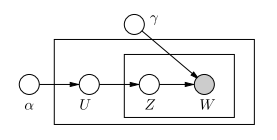
\includegraphics[width=.5\linewidth]{3-3.PNG}
    \caption{
        LDA 模型的图表示。
        单词变量 $W$ 为潜在主题 $Z$ 下的条件多元变量,其中 $\gamma$ 指定相应的分布。
        主题 $Z$ 也被建模为多元变量,分布以概率向量 $U$ 为参数,$U$ 服从参数为 $\alpha$ 的迪利克雷分布。
        该模型为层次贝叶斯模型的一个例子。
        这些矩形,也被称为盘(Plates),代表内部结构的重复。
    }\label{fig:3-3}
\end{figure}

很多图模型带有所谓的“硬核(Hard-core)”约束,这表示某些配置子集被禁止了。
这类问题的实例包括二元线性码的解码,以及其他组合优化问题(例如图匹配问题、覆盖问题、包装问题等)。
乍一看上去这样的分布族似乎不能使用指数族来表示,因为指数族中的密度 $p_{\theta}$ 都是严格正的——对于所有 $x \in \mathcal{X}^m$,都有 $p_{\theta}(x) > 0$。
在下面的例子中,我们将发现通过使用适当的基本测度 $\nu$ 可以将这些硬核约束融入到指数族框架中。

\begin{tcolorbox}
\begin{exam}[带有硬约束的模型]

产生硬核约束的一个重要领域是通信理论,特别是控错编码问题。
为了引出编码问题,假设有两个人——按照一个古老的惯例,称他们为爱丽丝和鲍勃——希望进行交流。
假设他们可以通过发送一串 01 序列进行通信,为了让问题变得具有研究意义,我们再假设连接双方的通信信道是随机的。
具体地说,在“位翻转(Bit-flipping)”信道中由爱丽丝发送的任何二进制数字都只有 $1-\epsilon$ 的概率被鲍勃正确接收。
该信道是一个概率模型,可以用条件分布来建模
$$p(y|x) \coloneqq \begin{cases}
    1 - \epsilon &\text{如果} x = y \\
    \epsilon &\text{如果} x \neq y
\end{cases}$$
其中 $x \in \{0, 1\}$ 代表爱丽丝发送的比特,$y \in \{0, 1\}$ 代表鲍勃接收的比特。

为了减少信道中的“噪声(Noisiness)”,爱丽丝和鲍勃约定以下的块编码(Block Coding)方案:不进行单个比特的传输,而是采用字节串 $(x_1, x_2, \dots, x_m)$ 进行通信,此外他们还约定只采用长度为 $m$ 总量为 $2^m$ 的字节串的一个子集。
这些特殊的字节串被称为编码字(Codewords),可以使用特定类型的图模型来定义。
具体来说,假设爱丽丝决定从满足一组校验的字节串 $x \in \{0, 1\}^m$ 中进行选择,校验形式假设为 $x_1 \oplus x_2 \oplus x_3 = 0$,其中 $\oplus$ 表示模 2 运算的加法。
考虑如下的奇偶检验集合 $F$,每一个 $a \in F$ 对一些比特子集 $N(a) \subset \{1, \dots, m\}$ 施加一个奇偶校验约束。
如果我们定义指示函数
\begin{equation}
    \psi_a(x_{N(a)}) \coloneqq \begin{cases}
        1 &\text{如果} \bigoplus_{i \in N(a)}x_i = 0 \\
        0 &\text{其他}
    \end{cases}
\end{equation}
那么二元线性码(Binary Linear Code)由满足 $\prod_{a \in F}\psi_a(x_{N(a)}) = 1$ 的所有字节串 $(x_1, x_2, \dots, x_m) \in \{0, 1\}^m$ 组成。
这些约束就是所谓的硬核约束,因为它们使得某些 $x$ 的取值概率为 0,也就把这些配置从分布的支撑集中清除了。
令 $(y_1, y_2, \dots, y_m) \in \{0, 1\}^m$ 表示鲍勃接收到的字节串,他的目的是利用这些观测结果来推断爱丽丝发送的是哪个编码字。
根据所使用的误差度量,这个解码问题对应于计算边际或者后验分布的众数
\begin{equation}
    p(x_1, \dots, x_m|y_1, \dots, y_m) \propto \prod_{i = 1}^mp(y_i|x_i)\prod_{a \in F}\psi_a(x_{N(a)})
\end{equation}
这种分布可以用因子图来表示,比特 $x_i$ 表示为非阴影圆形变量节点,观测值 $y_i$ 表示为阴影圆形变量节点,奇偶校验指示函数表示为方块因子节点(参见图 \ref{fig:2-9})。

这个图上的编码也可以被看作是一个指数族,只要我们对合适的基础测度取密度。
具体地说,我们可以使用奇偶校验来定义限制在有效编码字上的计数测度
\begin{equation}
    \nu(\{x\}) \coloneqq \prod_{a \in F}\psi_a(x_{N(a)})
\end{equation}
此外,由于观测值 $y_i$ 是固定的,因此条件分布 $p(y_i|x_i)$ 可以看作是 $x_i$ 的函数 $q(\cdot)$。
不用多少计算可以把这个函数写成如下指数形式
\begin{equation}
    q(x_i; \theta_i) = \exp\{\theta_ix_i - \log(1+\exp(\theta_i))\}
\end{equation}
其中指数参数 $\theta_i$ 由观测值 $y_i$ 与条件分布 $p(y_i|x_i)$ 定义为 $\theta_i = \log p(y_i|1)/p(y_i|0)$。
在二元对称信道的特殊情况下,这些标准参数可以写成
\begin{equation}
    \theta_i = (2y_i - 1)\log \frac{1-\epsilon}{\epsilon}
\end{equation}
需要注意的是我们将观测值向量 $(y_1, y_2, \dots, y_m)$ 看作是固定的。
在这样的条件下分布 (3.21) 可以作为一个指数族,其中密度是在限制计数测度 (3.22) 上定义的,形式为 $p_{\theta}(x|y) \propto \exp\{\sum_{i = 1}^m\theta_ix_i\}$。

\end{exam}
\end{tcolorbox}

\section{均值参数化和推断问题}

到目前为止,我们已经用标准参数向量 $\theta \in \Omega$ 刻画了任意指数族 $p_{\theta}$。
我们将在本节讨论任意指数族的均值参数(Mean Parameters)向量的替代参数化。
很多的统计计算,包括边缘化和最大似然估计,都可以理解为从一种参数表示到另一种参数表示的变换。

我们暂时离开主题,对边缘化问题中的观测变量或条件作用做一个评论。
如前所述,图模型的应用常常涉及到对随机变量(例如观测变量 $Y$)子集的约束,然后需要计算在后验分布 $p_{\theta}(x|y)$ 的边际。
例 3.6 中讨论的编码纠错就是这样的一个例子。
为了在接下来的讨论中简化表示,我们不再直接引用观测变量,而是只考虑指数族的无条件形式来讨论边缘化和其他计算问题。
这么做并不会损失一般性,因为观测变量的影响总可以通过适当地修正标准参数 $\theta$ 或充分统计量 $\phi$ 来解决。
(例如在例 3.6 中节点 $i$ 的噪声观测值 $y_i$ 为指数族分解提供了一个新的因子 $\exp(\theta_ix_i)$,如式 (3.23) 所示。)

\subsection{均值参数空间和边际多面体}

设 $p$ 为基本测度 $\nu$ 下的密度函数,我们暂时不假定 $p$ 为测度 $\nu$ 下的指数族。
与充分统计量 $\phi_{\alpha}: \mathcal{X}^m \rightarrow \mathbb{R}$ 相关的均值参数 $\mu_{\alpha}$ 定义为如下期望
\begin{equation}
    \mu_{\alpha} = \mathbb{E}_p[\phi_{\alpha}(X)] = \int \phi_{\alpha}(x)p(x)\nu(dx), \quad \forall \alpha \in \mathcal{I}
\end{equation}
通过这种方式,我们可以定义任意分布 $p$ 的均值参数向量 $(\mu_1, \dots, \mu_d)$,其中每个成分对应于一个充分统计量 $\phi_{\alpha}$($|\mathcal{I}| = d$)。
我们感兴趣的一个内容是向量 $u \in \mathbb{R}^d$ 随 $p$ 的改变而生成的轨迹空间。
正式而言,我们定义集合
\begin{equation}
    \mathcal{M} \coloneqq \{\mu \in \mathbb{R}^d| ~\exists ~p ~\text{s.t.} ~\mathbb{E}_p[\phi_{\alpha}(X)] = \mu_{\alpha}, ~\forall \alpha \in \mathcal{I}\}
\end{equation}
该集合包含了所有可能的均值参数。
值得注意的是,在这个定义中我们没有将密度 $p$ 限制为与充分统计量 $\phi$ 和基础测度 $\nu$ 相关的指数族。
然而在适当的条件下这个向量可以为指数族提供另一种参数化方法。

我们沿用前面一个例子来对这些概念进行说明:

\begin{tcolorbox}
\begin{exam}[高斯 MRF 的均值参数]

利用例 3.3 中高斯马尔可夫随机场的正则参数化(标准参数化),其充分统计量代表了均值参数,因此高斯马尔可夫随机场的均值参数为二阶矩矩阵 $\Sigma \coloneqq \mathbb{E}[XX^T] \in \mathbb{R}^{m \times m}$ 和均值向量 $\mu = \mathbb{E}[X] \in \mathbb{R}^m$。
对于这个特定的模型,可以直接给出所有可能的均值参数 $(\mu, \Sigma)$ 构成的集合 $\mathcal{M}$。
首先,如果 $(\mu, \Sigma)$ 是由某种分布(不一定非得是高斯)给出的,那么 $\Sigma - \mu\mu^T$ 一定是随机向量 $X$ 的一个有效协方差阵,这意味着半正定条件(Positive Semidefiniteness Condition,PSD)$\Sigma - \mu\mu^T \succeq 0$ 一定成立。
反之,对于任意满足 PSD 约束的 $(\mu, \Sigma)$,我们可以构造一个均值为 $\mu$,协方差(可能退化)为 $\Sigma - \mu\mu^T$ 的多元高斯分布,再从中导出 $(\mu, \Sigma)$。
到此为止,我们已经为高斯马尔可夫随机场建立了均值参数空间,$\mathcal{M}$ 的形式为
\begin{equation}
    \mathcal{M} = \{(\mu, \Sigma) \in \mathbb{R}^m \times \mathcal{S}_+^m| \Sigma - \mu\mu^T \succeq 0\}
\end{equation}
其中 $\mathcal{S}_+^m$ 代表 $m \times m$ 对称半正定矩阵集合。
图 \ref{fig:3-4} 给出了这个集合的标量实例($m = 1$),其中均值参数 $\mu = \mathbb{E}[X]$ 和 $\Sigma_{11} = \mathbb{E}[X^2]$ 必须满足二次约束 $\Sigma_{11} - \mu^2 \geq 0$。

\end{exam}
\end{tcolorbox}

\begin{figure}[htbp]
    \centering
    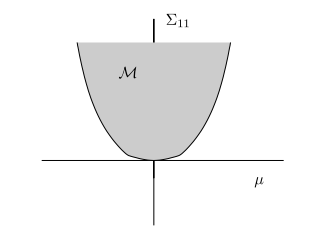
\includegraphics[width=.5\linewidth]{3-4.PNG}
    \caption{
        标量高斯的 $\mathcal{M}$ 集:这个模型具有两个均值参数 $\mu = \mathbb{E}[X]$ 和 $\Sigma_{11} = \mathbb{E}[X^2]$,必须满足二次约束 $\Sigma_{11} - \mu^2 \geq 0$。
        注意 $\mathcal{M}$ 是凸集,这个性质具有普遍性。
    }\label{fig:3-4}
\end{figure}

集合 $\mathcal{M}$ 总是 $\mathbb{R}^d$ 的一个凸子集。
可以证明,如果 $\mu$ 和 $\mu'$ 都是 $\mathcal{M}$ 中的元素,那么一定存在分布 $p$ 和 $p'$ 使得 $\mu = \mathbb{E}_p[\phi(X)]$ 且 $\mu' = \mathbb{E}_{p'}[\phi(X)]$。
对于任意 $\lambda \in [0, 1]$,凸组合 $\mu(\lambda) \coloneqq \lambda\mu + (1-\lambda)\mu'$ 一定可以由混合分布 $\lambda p + (1-\lambda)p'$ 导出,这就表明 $\mu(\lambda)$ 同样是 $\mathcal{M}$ 中的元素。
在附录 B.3 中,我们总结了集合 $\mathcal{M}$ 对于一般指数族都成立的一些性质。

离散随机变量的情况可以导出集合 $\mathcal{M}$ 的一些特殊性质。
具体来说,对于任意随机向量 $(X_1, X_2, \dots, X_m)$,与之相关的状态空间 $\mathcal{X}^m$ 是有限的,我们可以导出如下表示
\begin{align}
    \mathcal{M} &= \{\mu \in \mathbb{R}^d| ~\mu = \sum_{x \in \mathcal{X}^m}\phi(x)p(x), ~p(x) \geq 0, ~\sum_{x \in \mathcal{X}^m}p(x) = 1\} \nonumber \\
    &= conv\{\phi(x), x \in \mathcal{X}^m\} 
\end{align}
其中 $conv$ 代表凸包运算(参见附录 A.2)。
因此,当 $|\mathcal{X}^m|$ 有限时,集合 $\mathcal{M}$ 是一个凸多面体(Convex Polytope)。

附录 A.2 中的 Minkowski-Weyl 定理提供了凸多面体的另一种描述。
与有限向量集合的凸包不同,任意多面体 $\mathcal{M}$ 也可以由有限线性不等式约束集合来表征。
确切来说,对于任意多面体 $\mathcal{M}$,存在集合 $\{(a_j, b_j) \in \mathbb{R}^d \times \mathbb{R}| ~j \in \mathcal{J}\}$,
\begin{equation}
    \mathcal{M} = \{\mu \in \mathbb{R}^d| ~\langle a_j, \mu \rangle \geq b_j, ~\forall j \in \mathcal{J}\}
\end{equation}
其中 $|\mathcal{J}|$ 有限。
在几何上,这种表征代表 $\mathcal{M}$ 等于有限个半空间(Half-spaces)的交集,如图 \ref{fig:3-5} 所示。
接下来我们用伊辛模型来说明凸包表示 (3.28) 和线性不等式表示 (3.29) 之间的区别。

\begin{figure}[htbp]
    \centering
    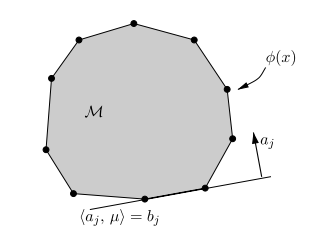
\includegraphics[width=.5\linewidth]{3-5.PNG}
    \caption{
        有限 $|\mathcal{X}^m|$ 下离散随机变量的集合 $\mathcal{M}$ 的图解。
        在这个例子中,集合 $\mathcal{M}$ 是一个与凸包 $\{\phi(x)| ~x \in \mathcal{X}^m\}$ 相关的凸多边形。
        根据 Minkowski-Weyl 定理,这个多边形也能写成有限个半空间的交集,每一个半空间的形式为 $\{\mu \in \mathbb{R}^d| ~\langle a_j, \mu \rangle \geq b_j\}$,$(a_j, b_j) \in \mathbb{R}^d \times \mathbb{R}$。
    }\label{fig:3-5}
\end{figure}

\begin{tcolorbox}
\begin{exam}[伊辛模型的均值参数]

例 3.1 中的伊辛模型的充分统计量为单例函数 $(x_s, s \in V)$ 和 成对函数 $(x_sx_t, (s, t) \in E)$。
充分统计量的向量形式如下:
\begin{equation}
    \phi(x) \coloneqq (x_s, s \in V; x_sx_t, (s, t) \in E) \in \mathbb{R}^{|V| + |E|}
\end{equation}
图 $G$ 的节点和边相应的均值参数对应于特定的边际概率:
\begin{subequations}
\begin{align}
    \mu_s &= \mathbb{E}_p[X_s] = \mathbb{P}[X_s = 1], \quad \forall s \in V \\
    \mu_{st} &= \mathbb{E}_p[X_sX_t] = \mathbb{P}[(X_s, X_t) = (1, 1)], \quad \forall (s, t) \in E
\end{align}
\end{subequations}
可见平均参数向量 $\mu \in \mathbb{R}^{|V|+|E|}$ 由单点上的边际概率($\mu_s$)和边上的成对边际概率($\mu_{st}$)组成。
集合 $\mathcal{M}$ 由 $\{\phi(x), x \in \{0, 1\}^m\}$ 的凸包组成,其中 $\phi(x)$ 由式 (3.30) 给出。
用概率的术语来说,$\mathcal{M}$ 对应于所有定义在 $(X_1, \dots, X_m) \in \{0, 1\}^m$ 上的单点与成对边际概率的集合。
在多面体组合学中,这个集合被称为相关多面体(Correlation Polytope)或者切割多面体(Cut Polytope)。

为了对这些概念有更具体的了解,接下来我们考虑最简单的非平凡情况:即一对连接在一起的变量 $(X_1, X_2)$ 以及它们构成的图。
在这个例子中,集合 $\mathcal{M}$ 是三维空间(两个节点加一条边)中的一个多面体:他是向量 $\{x_1, x_2, x_1x_2| (x_1, x_2) \in \{0, 1\}^2\}$ 的凸包,或者更准确一点
$$conv\{(x_1, x_2, x_1x_2)| (x_1, x_2) \in \{0, 1\}^2\}$$
参见图 \ref{fig:3-6}。

接下来我们考虑一下这个例子的半空间表示 (3.29)。
由初级概率论和一点点计算可以得到三个均值参数 $(\mu_1, \mu_2, \mu_3)$ 必须满足约束 $0 \leq \mu_{12} \leq \mu_i (i = 1, 2)$ 以及 $1+ \mu_{12} - \mu_1 -\mu_2 \geq 0$。
我们可以把这些约束写成矩阵-向量形式
$$\begin{bmatrix}
    0 & 0 & 1 \\
    1 & 0 & -1 \\
    0 & 1 & -1 \\
    -1 & -1 & 1
\end{bmatrix}\begin{bmatrix}
    \mu_1 \\
    \mu_2 \\
    \mu_{12}
\end{bmatrix} \geq \begin{bmatrix}
    0 \\
    0 \\
    0 \\
    -1
\end{bmatrix}$$
这四个约束为图 \ref{fig:3-6} 中的多面体提供了另一种表示形式。

\end{exam}
\end{tcolorbox}

\begin{figure}[htbp]
    \centering
    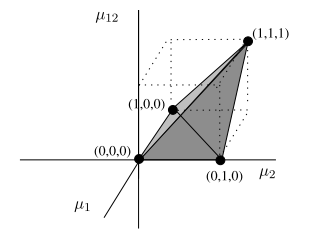
\includegraphics[width=.5\linewidth]{3-6.PNG}
    \caption{
        带有两个变量 $(X_1, X_2) \in \{0, 1\}^2$ 的伊辛模型的集合 $\mathcal{M}$。
        三个均值参数 $\mu_1 = \mathbb{E}[X_1]$,$\mu_2 = \mathbb{E}[X_2]$ 与 $\mu_{st} = \mathbb{E}[X_1X_2]$ 必须满足约束 $0 \leq \mu_{12} \leq \mu_i \quad i = 1, 2$ 以及 $1 + \mu_{12} - \mu_1 - \mu_2 \geq 0$。
        这些约束形成一个四面体,包含在单位超立方体 $[0, 1]^3$ 中。
    }\label{fig:3-6}
\end{figure}

下一个例子涉及纠错编码和二元拟阵理论(Binary Matroid Theory)中出现的一个多面体族:

\begin{tcolorbox}
\begin{exam}[编码字多面体与二元拟阵]

回顾一下例 3.6 中二元线性码的定义:它对应于满足奇偶校验关系
$$\mathbb{C} \coloneqq \{x \in \{0, 1\}^m| \prod_{a \in F}\psi_a(x_{N(a)}) = 1\}$$
的字节串 $x \in \{0, 1\}^m$ 的一个子集,其中每个奇偶校验函数作用在字节串子集 $N(a) \subset \{1, 2, \dots m\}$ 上。
将它视为指数族的时候,充分统计量就是 $\phi(x) = (x_1, x_2, \dots, x_m)$,基础测度为限制在集合 $\mathbb{C}$ 上的计数测度 $\nu$。
因此,这个问题的集合 $M$ 对应于编码字多边形(Codeword Polytope)——即所有编码字的凸包
\begin{align}
    \mathcal{M} &= conv\{x \in \{0, 1\}^m| \prod_{a \in F}\psi_a(x_{N(a)}) = 1\} \nonumber \\
    &= conv\{x \in \mathbb{C}\}
\end{align}

为了进一步做具体的说明,我们接下来考虑由单一奇偶校验关系 $x_1 \oplus x_2 \oplus x_3 = 1$ 定义的 $m = 3$ 位字节串。
图 \ref{fig:3-7}(a) 展示了这个玩具编码的因子图表示。
这个奇偶校验剔除了长度为 $3$ 的 $2^3 = 8$ 种可能字节串的一半取值。
编码字多面体即为 $\{(0, 0, 0), (0, 1, 1), (1, 0, 1), (1, 1, 0)\}$ 构成的凸包,如图 \ref{fig:3-7}(b) 所示,我们有可以使用半空间约束来表示该编码字多面体。
对于这个单奇偶校验码,编码字多面体由四个不等式定义
\begin{subequations}
\begin{align}
    (1-\mu_1) + (1-\mu_2) + (1-\mu_3) &\geq 1 \\
    (1-\mu_1) + \mu_2 + \mu_3 &\geq 1 \\
    \mu_1 + (1-\mu_2) + \mu_3 &\geq 1 \\
    \mu_1 + \mu_2 + (1-\mu_3) &\geq 1
\end{align}
\end{subequations}
这些不等式可以理解为 $(\mu_1, \mu_2, \mu_3)$ 离超立方体 $\{0, 1\}^3$ 的每个被奇偶校验码禁止的顶点的距离至少为 $1$,这点我们将在 8.4.4 小节详细讨论。

对于更长的、附有更多奇偶校验约束的二元线性码,相关的编码字多面体具有更复杂的结构。
编码字多面体在纠错编码问题中起着关键作用,在编码和信息领域对其进行了深入的研究。
任意二元线性码都可以使用二元拟阵来进行识别。
在这种情况下,编码字多面体被称为二元拟阵的循环多面体。
在组合学中,关于这些编码字有着丰富的研究文献。

\end{exam}
\end{tcolorbox}

\begin{figure}[htbp]
    \centering
    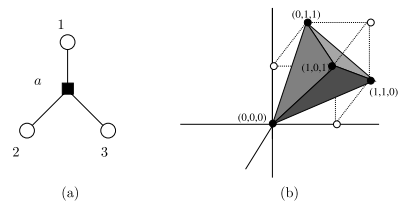
\includegraphics[width=.8\linewidth]{3-7.PNG}
    \caption{
        二元线性码特例 $\mathbb{C} = \{(0, 0, 0), (0, 1, 1), (1, 1, 0), (1, 0, 1)\}$ 相应的集合 $\mathcal{M}$。
        编码由一个简单的奇偶校验码定义。
    }\label{fig:3-7}
\end{figure}

例 3.8 和例 3.9 是某个很一般对象的实例,我们称其为离散图模型的边际多面体。
对于任意节点 $s \in V$ 都具有多元随机变量 $X_s \in \mathcal{X}_s \coloneqq \{0, 1, \dots, r_s-1\}$ 的图模型都可以定义边际多面体。
注意,基数 $|\mathcal{X}_s| = r_s$ 可以随节点而变。
考虑如下以 $\{0, 1\}$ 取值的指示函数所定义的指数族
\begin{align}
    \forall s \in V, j \in \mathcal{X}_s, \quad \mathbb{I}_{s;j}(x_s) &\coloneqq \begin{cases}
        1 & \text{如果} x_s = j \\
        0 & \text{其他}
    \end{cases} \nonumber \\
    \forall (s, t) \in E, (j, k) \quad \mathbb{I}_{st;jk}(x_s, x_t) &\coloneqq \begin{cases}
        1 & \text{如果} (x_s, x_t) = (j, k) \\
        0 & \text{其他}
    \end{cases}
\end{align}
我们将充分统计量 (3.34) 作为标准过完备表示(Standard Overcomplete Representation)。
其过完备性在例 3.2 中讨论过。

上述充分统计量可以使得均值参数具有非常直观的意义:对于每个节点 $s \in V$,都有
\begin{equation}
    \mu_{s;j} = \mathbb{E}_p[\mathbb{I}_j(X_s)] = \mathbb{P}[X_s = j], \quad \forall j \in \mathcal{X}_s
\end{equation}
对于每条边 $(s, t) \in E$
\begin{equation}
    \mu_{st;jk} = \mathbb{E}_p[\mathbb{I}_{st;jk}(X_s, X_t)] = \mathbb{P}[X_s = j, X_t = k], \quad \forall (j, k) \in \mathcal{X}_s \times \mathcal{X}_t
\end{equation}
因此,均值参数对应于节点的单例边际分布 $\mu_s$ 和边的成对边际分布 $\mu_{st}$。
在这种情况下,我们把集合 $\mathcal{M}$ 称为图对应的边际多面体(Marginal Polytope),记为 $\mathbb{M}(G)$。
具体地,它由下式给出
\begin{equation}
    \mathbb{M}(G) \coloneqq \{\mu \in \mathbb{R}^d| ~\exists ~p ~\forall (s; j) \text{满足式 (3.35)}, ~\forall (st; jk) \text{满足式 (3.36)}\}
\end{equation}

例 3.8 中的伊辛模型是边际多面体的一个特例,其节点变量 $X_s \in \{0, 1\}$。
唯一的区别在于边际多面体是在标准过完备指标函数的基础上定义的,而伊辛模型通常都可以参数化为最小指数族的形式。
例 3.9 中的编码字多面体是边际多面体的另一种特殊情况。
在这种情况下,约简需要两个步骤:首先,我们将编码的因子图表示——例如图 \ref{fig:3-7}(a)——转化为一个等价的成对马尔可夫随机场,每个位节点为二元变量,每个因子节点为高阶离散随机变量。
(从因子图转化为两两成对 MRFs 的详细步骤参见附录 E.3。)
和这个成对 MRF 相关的边际多面体只是编码字多面体的提升版。
我们将在后续的章节中更为详细地讨论这些边际多面体的例子。

对于例 3.8 和 3.9 中描述的两个模型,刻画边际多面体所需要的半空间约束的数目 $|\mathcal{J}|$ 非常小(两个例子都是 $|\mathcal{J}| = 4$)。
人们自然会问约束的数目是如何随着图的规模而变化的。
值得说明的是我们随后就能看到所谓的面复杂性(Facet Complexity)其实严重依赖于图结构。
对于树结构来说,任意边际多面体都具有局部约束的特征——只涉及边上的随机变量对——且总数只随图的规模线性增长。
与之形成鲜明对比的是,对于具有环的一般图,其约束是非局部的,并且其数目的增长速率快得惊人。
对于伊辛模型的特殊情况,可以参见 Deza 和 Laurent 的书,里面对相关多面体和切割多面体有详细的描述。
造成统计计算复杂性的一个根本原因在于表示边际多面体的方法是很紧凑的。

\subsection{均值参数在推断问题中的角色}

前面的例子表明均值参数在边际化问题中起着核心作用。
对于多元高斯(例 3.7),计算均值参数化的有效算法为我们提供了高斯均值向量和相关的协方差矩阵。
对于伊辛模型(例 3.8),均值参数完全给定了单点和成对的边际,这也适用于由标准过完备参数化 (3.34) 定义的多元图模型。
更一般地说,从正则参数 $\theta \in \Omega$ 到均值参数 $\mu \in \mathcal{M}$ 的前向映射(Forward Mapping)计算可以看做是指数族模型中推断问题的一个基本类(Fundamental Class)。
尽管对于大多数低维指数族映射的计算很简单,但是对于很多高维指数族来说,这个前向映射的计算极为困难。

反向映射(Backward Mapping),即从均值参数 $\mu \in \mathcal{M}$ 到正则参数 $\theta \in \Omega$ 也有自然的统计解释。
特别地,假设我们有一组样本 $X_1^n \coloneqq \{X^1, \dots, X^n\}$,它们是独立的采样自指数族 $p_{\theta}(x)$,其中 $\theta$ 未知。
如果我们想要估计 $\theta$ 的值,那么根据经典的最大似然原理我们可以通过最大化数据的似然来获得估计值 $\hat{\theta}$,也可以通过取对数等价地最大化量
\begin{equation}
    l(\theta; X_1^n) \coloneqq \frac{1}{n}\sum_{i = 1}^n\log p_{\theta}(X^i) = \langle \theta, \hat{\mu} \rangle - A(\theta)
\end{equation}
其中 $\hat{\mu} \coloneqq \hat{\mathbb{E}}[\phi(X)] = \frac{1}{n}\sum_{i = 1}^n\phi(X^i)$ 为由数据 $X_1^n$ 定义的经验均值参数(Empirical Mean Parameters)向量。
最大似然估计量 $\hat{\theta}$ 是对这个目标函数最大化的解。
需要注意的是,一般而言计算 $\hat{\theta}$ 也是一个难题,因为目标函数中涉及到了对数配分函数 $A$。
下面将会证明,在合适的条件下,最大似然估计量是唯一的,且由统计条件 $\mathbb{E}_{\hat{\theta}}[\phi(X)] = \hat{\mu}$ 确定。
找到这个等式的唯一解等价于计算反向映射 $\mu \mapsto \theta$,从均值参数到正则参数。
一般而言,这个反向映射也需要大量的计算。

\section{对数配分函数 $A$ 的性质}

指数族由四个核心部分组成,充分统计量、正则参数、均值参数以及累积函数(对数配分函数),前三个我们已经有所讨论,现在我们来深入讨论累积函数 $A$ 的一些性质。
$A$ 最重要的性质可能是它的凸性,这是凸分析的领域,其中最重要的是共轭对偶性。
在适当的条件下,函数 $A$ 和它的共轭对偶 $A^*$ ——或者更准确一点地说是他们的导数——在正则参数和均值参数之间建立了一一对应的双射关系。
如前所述,正则参数和均值参数之间的映射关系是高维图模型中各种统计计算的核心挑战。

\subsection{导数和凸性}

回顾一下凸函数的概念,对于一个实值函数 $g$,如果其定义域内任意两个元素 $x, y$ 和任意标量 $\lambda \in (0, 1)$ 满足下列不等式
\begin{equation}
    g(\lambda x + (1-\lambda)y) \leq \lambda g(x) + (1-\lambda)g(y)
\end{equation}
那么 $g$ 是一个凸函数。
从几何的角度来看,这个不等式意味着连接函数值 $g(x)$ 和 $g(y)$ 的线段位于函数图像之上。
如果不等式 (3.39) 对任意 $x \neq y$ 都严格成立,那么这个函数是严格凸(Strictly Convex)的。
(凸函数一些其他的性质参见附录 A.2.5。)
我们先证明对数配分函数在 $\theta$ 上是光滑的、凸的。

\begin{tcolorbox}
\begin{prop}

与任意正则指数族相关的累积函数
\begin{equation}
    A(\theta) \coloneqq \log \int_{\mathcal{X}^m}\exp\langle \theta, \phi(x) \rangle \nu(dx)
\end{equation}
都具有以下性质:

\begin{itemize}
    \item[(a)] 在定义域 $\Omega$ 内具有任意阶导数。
        头两阶导数可以导出随机向量如下累积量(Cumulants):
        \begin{subequations}
        \begin{align}
            \frac{\partial A}{\partial \theta_{\alpha}}(\theta) &= \mathbb{E}_{\theta}[\phi_{\alpha}(X)] \coloneqq \int \phi_{\alpha}(x)p_{\theta}(x)\nu(dx) \\
            \frac{\partial^2 A}{\partial\theta_{\alpha}\partial\theta_{\beta}}(\theta) &= \mathbb{E}_{\theta}[\phi_{\alpha}(X)\phi_{\beta}(X)] - \mathbb{E}_{\theta}[\phi_{\alpha}(x)]\mathbb{E}_{\theta}[\phi_{\beta}(X)]
        \end{align}
        \end{subequations}
    \item[(b)] 此外,$A$ 对 $\theta$ 在其定义域 $\Omega$ 内是凸函数,且在最小表示的情况下是严格凸的。
\end{itemize}

\end{prop}
\end{tcolorbox}

\analysis[证明]
我们假设对 $A$ 的积分定义式 (3.40) 可以进行求导,这个假设可以由支配收敛定理(Dominated Convergence Theorem)得到。
基于这个假设我们有
\begin{align*}
    \frac{\partial A}{\partial \theta_{\alpha}}(\theta) &= \frac{\partial}{\partial \theta_{\alpha}}\{\log\int_{\mathcal{X}^m}\exp\langle\theta, \phi(x)\rangle\nu(dx)\} \\
    &= \frac{[\int_{\mathcal{X}^m}\frac{\partial}{\partial\theta_{\alpha}}\exp\langle\theta, \phi(x)\rangle\nu(dx)]}{[\int_{\mathcal{X}^m}\exp\langle\theta, \phi(x)\rangle\nu(dx)]} \\
    &= \int_{\mathcal{X}^m}\phi_{\alpha}(x)\frac{\exp\langle\theta, \phi(x)\rangle\nu(dx)}{\int_{\mathcal{X}^m}\exp\langle\theta, \phi(u)\rangle\nu(du)} \\
    &= \mathbb{E}_{\theta}[\phi_{\alpha}(X)]
\end{align*}
这就导出了式 (3.41a)。
高阶导数的公式可以用类似的方式进行证明。

观察式 (3.41b) 可知二阶偏导 $\frac{\partial^2A}{\partial\theta_{\alpha}\partial\theta_{\beta}}$ 与协方差元素 $cov\{\phi_{\alpha}(X), \phi_{\beta}(X)\}$ 相等。
因此整个黑塞矩阵(Hessian)$\nabla^2A(\theta)$ 就是随机向量 $\phi(X)$ 的协方差矩阵,其在开集 $\Omega$ 上为半正定的,也就保证了函数的凸性。
如果采用的是最小表示,那么就不存在非零向量 $a \in \mathbb{R}^d$ 和常数 $b \in \mathbb{R}$ 使得 $\langle a, \phi(x)\rangle = b$ 在基础测度 $\nu$ 上几乎处处成立。
这也就表示对于所有的 $a \in \mathbb{R}^d$ 和 $\theta \in \Omega$ 都有 $var_{\theta}[\langle a, \phi(x)\rangle] = a^T\nabla^2A(\theta)a > 0$。
黑塞矩阵在开集 $\Omega$ 上的严格正定意味着函数的严格凸性。
\qed

\subsection{转向均值参数的前向映射}

我们现在来深度探索一下前向映射 $\theta \mapsto \mu$,从正则参数 $\theta \in \Omega$ 定义的分布 $p_{\theta}$ 到与之相关的均值参数向量 $\mu \in \mathbb{R}^d$。
注意到梯度 $\nabla A$ 是一个从 $\Omega$ 到 $\mathbb{R}^d$ 的映射。
命题 3.1 证明了该映射的值域包含在先前定义的可实现的均值参数集合 $\mathcal{M}$ 内
$$\mathcal{M} \coloneqq \{\mu \in \mathbb{R}^d| ~\exists ~p ~s.t. ~\mathbb{E}_p[\phi(X)] = \mu\}$$
以下两个问题对这个映射提出了更深刻的内涵:

\begin{itemize}
    \item[(a)] $\nabla A$ 在什么情况下是一个一一映射?
    \item[(b)] $\Omega$ 在映射 $\nabla A$ 下的像——也就是集合 $\nabla A(\Omega)$ ——在什么情况下覆盖整个集合 $\mathcal{M}$?
\end{itemize}

第一个问题的答案很明了,就是取决于这个指数族是不是最小的。
第二个问题有点微妙:首先需要注意的是,我们在 $\mathcal{M}$ 的定义中均值参数 $\mu \in \mathbb{R}^d$ 可以由任意可能的分布生成,而不仅仅只是充分统计量 $\phi$ 所定义的指数族。
事实证明这个额外的自由度并没有扩大集合 $\mathcal{M}$,正如命题 3.3 所指出的那样,在适当的条件下 $\mathcal{M}$ 中的所有均值参数都可以由指数族分布来实现(边界点可以由这种分布的极限序列来实现)。

我们首先给出第一个问题的答案:

\begin{tcolorbox}
\begin{prop}

当且仅当指数族是最小表示的时候梯度映射 $\nabla A: \Omega \rightarrow \mathcal{M}$ 是一一对应的。

\end{prop}
\end{tcolorbox}

\analysis[证明]
如果表示不是最小的,那么一定存在一个非零向量 $\gamma \in \mathbb{R}^d$ 使得 $\langle \gamma, \phi(x) \rangle$ 在测度 $\gamma$ 上几乎处处为常数。
给定任意一个参数 $\theta^1 \in \Omega$,定义另一个参数向量 $\theta^2 = \theta^1 + t\gamma$,其中 $t \in \mathbb{R}$。
因为 $\Omega$ 为开集,可以选择一个充分小的 $t$ 使得 $\theta^2 \in \Omega$。
在 $\gamma$ 的条件下,密度 $p_{\theta^1}$ 和 $p_{\theta^2}$ 包含相同的概率分布(只是它们的归一化常数不同)。
在这一对上有 $\nabla A(\theta^1) = \nabla A(\theta^2)$,因此 $\nabla A$ 并不是一一对应的。

相反如果表示是最小的,那么根据命题 3.1 $A$ 是严格凸的。
对于任何严格凸可微函数,我们有 $A(\theta^2) > A(\theta^2) + \langle \nabla A(\theta^1), \theta^2-\theta^1 \rangle, \forall \theta^1 \neq \theta^2 \in \Omega$。
调换 $\theta^1$ 和 $\theta^2$ 的位置不等式同样成立。
把这两个不等式加起来可以得到
$$\langle \nabla A(\theta^1) - \nabla A(\theta^2), \theta^1 - \theta^2 \rangle > 0$$
这个不等式对任意不相等的 $\theta^1, \theta^2 \in \Omega$ 都成立,这表明 $\nabla A$ 是一一对应的。
\qed

一般而言,尽管对于过完备表示的梯度映射 $\nabla A$ 并不是一一对应的,但是在 $\nabla A(\Omega)$ 的每个元素和 $\Omega$ 的一个仿射子集之间仍然存在一种一一对应的关系。
具体说来,一个仿射子集就是由映射到同一个均值参数的正则参数组成。
无论是最小表示还是过完备表示,如果 $\mu = \nabla A(\theta)$,那么我们说 $(\theta, \mu)$ 是对偶(Dually Coupled)的。
这个对偶概念在后续的内容里面扮演着重要的角色。

现在我们转向第二个问题,有效正则参数域 $\Omega$ 在梯度映射 $\nabla A$ 下的像 $\nabla A(\Omega)$。
具体说来,这个问题的目标就是确定对于均值向量 $\mu \in \mathcal{M}$ 来说是否存在向量 $\theta = \theta(\mu) \in \Omega$ 满足 $\mathbb{E}_{\theta}[\phi(X)] = \mu$。
这个问题的解其实也很简单:像 $\nabla A(\Omega)$ 只是内点集(Interior) $\mathcal{M}^\circ$。
这个事实值得注意,因为它意味着除了边界点之外的所有均值参数 $\mathcal{M}$ 都可以由指数族的某个成员实现。
为了给这个事实一个直观的解释,给定 $\mathcal{M}$ 中的一个内点均值参数 $\mu$,我们来考虑最大熵问题 (3.3)。
如前所述,如果这个问题的解存在,那么它也必须采用指数族的形式 $p_{\theta}(\mu)$。
此外,从最大熵问题的最优性条件来看,该指数族必须满足矩匹配条件(Moment-matching)$\mathbb{E}_{\theta(\mu)}[\phi(X)] = \mu$。
需要注意的是这些矩匹配条件与定义最大似然问题 (3.38) 的条件是相同的——这一点我们将在下一节中进行讨论,这个事实不是巧合,而是最大熵和最大似然之间的原始-对偶(Primal-Dual)关系的一个结论。

\begin{tcolorbox}
\begin{prop}

在一个最小表示的指数族中,梯度映射 $\nabla A$ 的像是 $\mathcal{M}$ 的内点集,记为 $\mathcal{M}^\circ$。
因此,对于每个 $\mu \in \mathcal{M}^\circ$,都存在某个 $\theta = \theta(\mu) \in \Omega$ 满足 $\mathbb{E}_{\theta}[\phi(X)] = \mu$。

\end{prop}
\end{tcolorbox}

我们在附录 B 中给出了这个结论的证明。
结合命题 3.2,命题 3.3 保证了最小指数族中每个均值参数 $\mu \in \mathcal{M}^\circ$ 都可以由指数族的某个成员密度 $p_{\theta(\mu)}$ 唯一实现。
然而一个典型的指数族 $\{p_{\theta}| \theta \in \Omega\}$ 仅仅描述所有基础测度 $\nu$ 下可能密度的一个严格子集。
在这种情况下,至少也存在一些非指数族的密度 $p$ 能够实现 $\mu$。
指数分布族 $p_{\theta(\mu)}$ 的特点是在所有实现 $\mu$ 的分布集合中具有最大的熵。
$A$ 与最大熵原理的联系可以用共轭对偶函数 $A^*$ 来表示,我们接下来就来讨论它。

\section{共轭对偶:最大似然与最大熵}

共轭对偶(Conjugate Duality)是凸分析的基础,可以通过它自然地导出变分表示。
本节我们讨论对数配分函数 $A$ 和共轭对偶函数 $A^*$ 的关系。
这种共轭关系是由变分原理所决定的,变分原理是本书剩余内容的核心,可以导出各种已知的算法,不论是精确的(例如联合树算法以及它的特例卡尔曼滤波、前后向算法和剥离算法)还是近似的(例如带环图的和积算法、平均场、期望传播、菊池方法、线性规划和半定松弛)。

\subsection{共轭对偶的一般形式}

给定一个函数 $A$,其共轭对偶函数 $A^*$ 定义如下:
\begin{equation}
    A^*(\mu) \coloneqq \sup_{\theta \in \Omega}\{\langle \mu, \theta \rangle - A(\theta)\}
\end{equation}
其中 $\mu \in \mathbb{R}^d$ 为一个固定向量,称为对偶变量,维度和 $\theta$ 相同。
我们选择 $\mu$ 来表示对偶变量是有意为之,因为这些对偶变量就蕴含着均值参数的意义。
事实上,我们已经提到了变分问题 (3.42) 的一种统计解释,右侧就是对数似然 (3.38) 的最优值。
当然,这个最大似然问题只有当向量 $\mu$ 属于 $\mathcal{M}$ 时才有意义,由数据集 $X_1^n = \{X^1, \dots, X^n\}$ 诱导的经验矩矢量 $\hat{\mu} = \frac{1}{n}\sum_{i = 1}^n\phi(X^i)$ 就是一个例子。
我们将优化问题 (3.42) 考虑得更为广泛,包含了任意向量 $\mu \in \mathbb{R}$。
在这种条件下,有必要将 $A^*$ 看作为在拓展实线 $\mathbb{R}^* = \mathbb{R} \cup \{+\infty\}$ 上取值的函数,正如标准的凸分析中一样(参见附录 A.2.5)。

如前所述,共轭对偶函数 (3.42) 与熵密切相关。
回想一下香农熵的定义 (3.2)。
定理 3.4 的主要结果是:当 $\mu \in \mathcal{M}^\circ$ 时,对偶函数 $A^*(\mu)$ 的值恰好是指数分布族 $p_{\theta(\mu)}$ 的负熵,其中 $\theta(\mu)$ 是满足满足关系
\begin{equation}
    \mathbb{E}_{\theta(\mu)}[\phi(X)] = \nabla A(\theta(\mu)) = \mu
\end{equation}
的唯一正则参数向量。
我们也会考虑 $\mu \notin \mathcal{M}^\circ$ 的情况,在这种情况下不可能找到满足关系 (3.43) 的正则参数。
在这种情况下,我们需要对 $A^*(\mu)$ 上界的定义进行更为细致的分析。
事实上,令 $\overline{\mathcal{M}}$ 表示 $\mathcal{M}$ 的闭包,如果 $\mu \notin \overline{\mathcal{M}}$,那么 $A^*(\mu) = +\infty$。
这个事实对于变分方法的使用是至关重要的:它保证任何涉及对偶函数的优化问题可以被简化为一个 $\mathcal{M}$ 上的优化问题。
因此在后续的章节中,我们将大量讨论各种图模型的 $\mathcal{M}$ 结构,如果 $\mathcal{M}$ 的结构过于复杂,我们将会讨论它的近似。

更正式地说,以下在附录 B.2 证明的命题提供了 $A$ 和它的共轭对偶 $A^*$ 之间的关系:

\begin{tcolorbox}
\begin{prop}

\begin{itemize}
    \item[(a)] 对于任意 $\mu \in \mathcal{M}^\circ$,令 $\theta(\mu)$ 表示唯一满足对偶匹配条件 (3.43) 的正则参数
        共轭对偶函数 $A^*$ 具有如下形式
        \begin{equation}
            A^*(\mu) = \begin{cases}
                -H(p_{\theta(\mu)}) & \text{如果} \mu \in \mathcal{M}^\circ \\
                +\infty & \text{如果} \mu \notin \overline{\mathcal{M}}
            \end{cases}
        \end{equation} 
        对于任意边界点 $\mu \in \overline{\mathcal{M}}\setminus\mathcal{M}^\circ$ 我们有 $A^*(\mu) = \lim_{n \to +\infty}A^*(\mu^n)$,其中序列 $\{\mu^n\} \subset \mathcal{M}^\circ$ 收敛到 $\mu$。
    \item[(b)] 在对偶的术语中,对数配分函数也有变分表示
        \begin{equation}
            A(\theta) = \sup_{\mu \in \mathcal{M}}\{\langle\theta, \mu\rangle - A^*(\mu)\}
        \end{equation}
    \item[(c)] 对于所有 $\theta \in \Omega$,式 (3.45) 的上界由满足矩匹配条件
        \begin{equation}
            \mu = \int_{\mathcal{X}^m}\phi(x)p_{\theta}(x)\nu(dx) = \mathbb{E}_{\theta}[\phi(X)]
        \end{equation}
        的唯一向量 $\mu \in \mathcal{M}^\circ$ 取到。
\end{itemize}

\end{prop}    
\end{tcolorbox}

命题 3.4(a) 说明了累积函数 $A$ 和熵之间的对偶性。
接下来对这种关系做如下说明。
第一,有必要认识到 $A^*$ 和通常意义上的熵 (3.2) 有着些许不同:鉴于熵将密度函数映射到实数(因此是一个泛函),对偶函数 $A^*$ 是 $\mathbb{R}^d$ 上的一个拓展实值函数,仅对有效的均值参数 $\mu \in \mathcal{M}$ 有限。

第二,$-A^*(\mu)$ 的值与最大熵问题 (3.3) 的优化值有关,其中 $\mu \in \mathbb{R}^d$ 对约束集进行了参数化。
事件 $A^*(\mu) = +\infty$ 对应于最大熵问题的不可行性。
这是很重要的一点。
约束优化问题是由被优化的集合与被优化的函数定义的。
累积函数的变分表示 (3.45) 采用了最大化问题的形式,我们可以看到满足 $-A^*(\mu) = -\infty$ 的向量 $\mu$ 肯定不是最优解。
因此我们在变分表示 (3.45) 中是对集合 $\mathcal{M}$ 实行最大化而不是 $\mathbb{R}^d$。
这意味着集合 $\mathcal{M}$ 的性质是决定累积函数计算复杂性的关键。

第三,命题 3.4 也阐明了集合 $\Omega$ 和 $\mathcal{M}^\circ$ 之间双射关系的精确性质,这一点适用于所有最小指数族。
特别地,梯度映射 $\nabla A$ 以一一对应的形式将 $\Omega$ 映射到 $\mathcal{M}^\circ$,而对偶函数的梯度 $\nabla A^*$ 则表征了从 $\mathcal{M}^\circ$ 到 $\Omega$ 的逆映射(参见附录 B.3)。
图 \ref{fig:3-8} 展示了基于梯度映射 $(\nabla A, \nabla A^*)$ 的双射关系。

\begin{figure}[htbp]
    \centering
    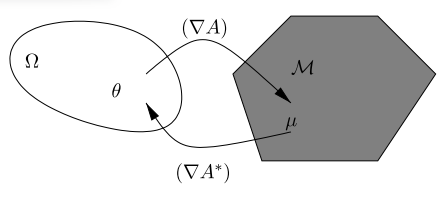
\includegraphics[width=.8\linewidth]{3-8.PNG}
    \caption{
        有效正则参数集合 $\Omega$ 与有效均值参数集合 $\mathcal{M}$ 之间的关系。
        与共轭对偶对 $(A, A^*)$ 相关的梯度映射 $\nabla A$ 和 $\nabla A^*$ 提供了 $\Omega$ 与内点集 $\mathcal{M}^\circ$ 之间的一个双射关系。
    }\label{fig:3-8}
\end{figure}

\subsection{一些简单的例子}

通过一些简单的例子可以很好地理解命题 3.4。
表 \ref{tab:3-2} 提供了几个已知的标量随机变量指数族的共轭对偶 $(A, A^*)$。
对于每个族,该表还列出了 $\Omega \coloneqq dom A$ 以及 $A^*$ 的有效域 $\mathcal{M}$,在这个集合中 $A^*$ 的值是有限的。

\begin{sidewaystable}[htbp]
\caption{
    几个常见的标量指数族的共轭对偶关系
}\label{tab:3-2}
\centering
\begin{tabular}{lcccc}
    \hline
    Family & $\Omega$ & $A(\theta)$ & $\mathcal{M}$ & $A^*(\mu)$ \\
    \hline
    Bernoulli & $\mathbb{R}$ & $\log[1+\exp(\theta)]$ & $[0, 1]$ & $\mu\log\mu + (1-\mu)\log(1-\mu)$ \\
    Gaussian & $\mathbb{R}$ & $\frac{1}{2}\theta^2$ & $\mathbb{R}$ & $\frac{1}{2}\mu^2$ \\
    Gaussian & $\{(\theta_1, \theta_2)| \theta_2 < 0\}$ & $-\frac{\theta_1^2}{4\theta_2^2} - \frac{1}{2}\log{(-2\theta_2)}$ & $\{(\mu_1, \mu_2)| \mu_2 - (\mu_1)^2 > 0\}$ & $-\frac{1}{2}\log[\mu_2 - \mu_1^2]$ \\
    Exponential & $(-\infty, 0)$ & $-\log(-\theta)$ & $(0, +\infty)$ & $-1 - \log\mu$ \\
    Poison & $\mathbb{R}$ & $\exp(\theta)$ & $(0, +\infty)$ & $\mu\log\mu -\mu$ \\
    \hline
\end{tabular}
\end{sidewaystable}

这一小节的剩余部分我们将讨论两个标量的例子。
需要明确的是,从计算的角度来看这两个例子都很平凡——实际上对于大多数标量指数族来说,可以很简单地直接计算正则参数和均值参数之间的映射。
尽管如此,它们还是有助于建立对命题 3.4 的直观理解。
只对主线感兴趣的读者可以直接跳到 3.7 小节,在那里我们将继续对命题 3.4 在推导多元指数族近似推断算法中的作用进行讨论。

\begin{tcolorbox}
\begin{exam}[伯努利模型的共轭对偶性]
    
考虑一个伯努利变量 $X \in \{0, 1\}$:它的分布可以写成指数族的形式,其中 $\phi(x) = x$,$A(\theta) = \log(1+\exp(\theta))$,$\Omega = \mathbb{R}$。
为了验证命题 3.4(a),我们直接计算共轭对偶函数 $A^*$。
通过共轭对偶的定义式 (3.42),对于任意固定的 $\mu \in \mathbb{R}$,我们有
\begin{equation}
    A^*(\mu) = \sup_{\theta \in \mathbb{R}}\{\theta\cdot\mu - \log(1+\exp(\theta))\}
\end{equation}
求导得到驻点条件 $\mu = \exp(\theta)/[1+\exp(\theta)]$,也就是矩匹配条件 (3.43) 在伯努利模型中的特例。
驻点条件在什么情况下有解呢?
如果 $\mu \in (0, 1)$,那么通过一些简单的代数运算我们可以得到唯一解 $\theta(\mu) \coloneqq \log[\mu/(1-\mu)]$。
因为对于伯努利模型来说 $\mathcal{M}^\circ = (0, 1)$,解的存在唯一性就是命题 3.2 和 3.3 的结论。
因为目标函数 (3.47) 是严格凸的,解 $\theta(\mu)$ 就是最优的,将 $\theta(\mu)$ 代入目标式 (3.47) 化简可得
\begin{align*}
    A^*(\mu) &= \mu\log[\frac{\mu}{1-\mu}] - \log[1+\frac{\mu}{1-\mu}] \\
    &= \mu\log\mu + (1-\mu)\log(1-\mu)
\end{align*}
这个就是均值参数为 $\mu$ 的伯努利变量的负熵。
至此我们就验证了在 $\mu \in (0, 1) = \mathcal{M}^\circ$ 情况下的命题 3.4(a)。

现在我们来考虑 $\mu \notin \overline{\mathcal{M}} = [0, 1]$ 的情况,具体地,我们假设 $\mu > 1$。
在这种情况下,优化问题 (3.47) 不存在梯度驻点。
因此上界只能通过取极限 $\theta \to \pm\infty$ 得到。
对于 $\mu > 1$,我们可以得到目标函数在 $\theta \to +\infty$ 时无界。
确实,由 $A$ 的凸性可得 $A(0) = \log 2 \geq A(\theta) + A'(\theta)(-\theta)$。
此外对于所有 $\theta \in \mathbb{R}$ 都有 $A'(\theta) \leq 1$,可得对于 $\theta > 0$ 有 $A(\theta) \leq \theta + \log 2$。
因此对于任意 $\theta > 0$ 我们有
$$\mu\cdot\theta - \log[1+\exp(\theta)] \geq (\mu-1)\theta - \log 2$$
这说明当 $\mu > 1$ 时,目标函数在 $\theta \to +\infty$ 处发散。
同理可得 $\mu < 0$ 的情况,表明 $\mu \notin \overline{\mathcal{M}}$ 时 $A^*(\mu) = +\infty$,证明了命题 3.4(a) 的第二部分。
最后对于边界点 $\mu = 0$ 和 $\mu = 1$,对伯努利模型我们取极限可以得到 $A^*(0) = A^*(1) = 0$。

对于命题 3.4(b) 的验证,由于除非 $\mu \in [0, 1]$, $A^*(\mu) = +\infty$,因此优化问题 (3.45) 简化为
$$\max_{\mu \in [0, 1]}\{\mu\cdot\theta - \mu\log\mu - (1-\mu)\log(1-\mu)\}$$
求解这个凹最大化问题可得其最优值 $\log[1+\exp(\theta)]$,这就证明了命题 3.4(b)。
同理可得最优解 $\mu(\theta) = \exp(\theta)/[1+\exp(\theta)]$ 是唯一的,这就证明了伯努利模型的命题 3.4(c)。

\end{exam}
\end{tcolorbox}

\begin{tcolorbox}
\begin{exam}[指数模型的共轭对偶]
    
考虑指数分布,其指数族形式为 $\phi(x) = x$,$\Omega = (-\infty, 0)$,$A(\theta) = -\log(-\theta)$。
由共轭对偶定义式 (3.42) 可得
\begin{equation}
    A^*(\mu) = \sup_{\theta < 0}\{\mu\cdot\theta + \log(-\theta)\}
\end{equation}
为了得到最优解,我们对 $\theta$ 求导。
我们可以得到驻点条件 $\mu = -1/\theta$,也就是指数分布的矩匹配条件 (3.43)。
因此,对于所有的 $\mu \in \mathcal{M}^\circ = (0, \infty)$,我们有 $A^*(\mu) = -1 - \log(\mu)$。
可以验证 $\mu > 0$ 的指数分布的熵就是 $-A^*(\mu)$。
这就验证了 $\mu \in \mathcal{M}^\circ$ 的命题 3.4。
对于 $\mu \notin \overline{\mathcal{M}}$ ——也就是 $\mu < 0$ ——我们可以验证目标函数 $\mu\theta + \log(-\theta)$ 在 $\theta \to -\infty$ 时无界,从而对于所有 $\mu \notin \mathcal{M}$ 都有 $A^*(\mu) \to +\infty$。
剩下的边界点 $\mu = 0$ 通过定义式 (3.48) 可得 $A*(0) = +\infty$。
还需要注意的是,指数分布 $-1-\log(\mu_n)$ 的负熵对于所有序列 $\mu^n \to 0^+$ 都趋于无穷,这与命题 3.4(a) 一致。
得到对偶 $A^*$ 之后,通过简单的计算就可以得到
$$A(\theta) = -\log(-\theta) = \sup_{\mu > 0}\{\mu\cdot\theta + 1 + \log(\mu)\}$$
最优值在 $\mu = -1/\theta$ 取到。
这就证明了指数分布的命题 3.4(b) 和 (c)。

\end{exam}
\end{tcolorbox}

\section{高维模型的计算困难}

从计算的角度来看,命题 3.4 的基本特性是累积函数的表示 (3.45),以及在均值参数取值 $\mu = \mathbb{E}_{\theta}[\phi(X)]$ 时达到最优的断言 (3.46)。
这表明累积函数 $A$ 和均值参数 $\mu$ 的计算有一个关键的性质:原则上我们可以通过求解变分问题 (3.45) 来计算这两个量。
更令人鼓舞的是,这个优化问题至少从表面上看起来很简单:它是一个凸集上的有限维优化问题,目标函数严格凹且可微。
因此这个优化问题没有局部最优或者其他不好的特性。
这么看来对数配分函数和相关均值参数的计算问题已经解决了,因为我们已经把它“简化”为一个凸优化问题。

在这种情况下,表 \ref{tab:3-2} 中简单的标量例子非常容易误导人,因为它的基本变分问题 (3.45) 有显式解,很容易解决。
相比之下,对于一般的多元指数族,变分表示主要有两个挑战:

\begin{itemize}
    \item[(a)] 在许多情况下,可实现的均值参数约束集合 $\mathcal{M}$ 很难有显式的表征。
    \item[(b)] 负熵函数 $A^*$ 是以一种变分的方式间接定义的,它也同样很难有显式表征。
\end{itemize}

举个例子来说明问题 (a) 提到的 $\mathcal{M}$ 的性质,对于具有离散随机变量 $X \in \{0, 1, \dots, r-1\}^m$ 的马尔可夫随机场,集合 $\mathcal{M}$ 总是一个多面体,也就是我们之前所说的边际多面体。
在这种情况下,集合 $\mathcal{M}$ 至少在原则上可以用有限个线性不等式来刻画。
然而对于一般的图模型来说,这样的不等式随着图模型规模的增长而不断增多。
事实上,除非复杂性理论中的基本猜想被证明是错误的,否则对于一般的离散 MRF 来说在 $\mathcal{M}$ 上优化一个线性函数都是不可能的。
除了约束集合的复杂性之外,问题 (b) 还强调了即使评估单个点 $\mu \in \mathcal{M}$ 的代价函数都是极其困难的,更别说在 $\mathcal{M}$ 上对其进行优化。

为了理解对偶值 $A^*(\mu)$ 的复杂性,注意命题 3.4 只提供了 $A^*$ 一种作为复合映射的隐表征:首先是将 $\mu$ 映射到 $\theta(\mu)$ 的逆映射 $(\nabla A)^{-1}: \mathcal{M}^\circ \to \Omega$,与均值参数为 $\mu$ 的指数族成员相关;其次是从 $\theta(\mu)$ 到相关指数族密度的负熵 $-H(p_{\theta(\mu)})$ 的映射。
$A^*(\mu)$ 值的分解如图 \ref{fig:3-9} 所示。
因此在某个点 $\mu \in \mathcal{M}$ 处计算对偶值 $A^*(\mu)$ 需要计算逆映射 $(\nabla A)^{-1}(\mu)$,这个就已经不简单了,然后再计算熵,这在一般图模型上需要进行高维积分。
这些难点导致需要对 $\mathcal{M}$ 和 $A^*$ 寻求近似。
实际上,如下一章节所示,一大类近似边际化方法都是以对精确变分的近似,然后通过某种消息传递算法来实现的。

\begin{figure}[htbp]
    \centering
    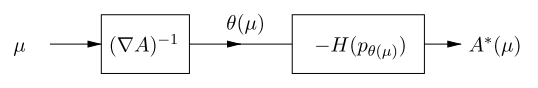
\includegraphics[width=.8\linewidth]{3-9.PNG}
    \caption{
        $A^*$ 作为两个函数复合的分解方块图。
        一个均值参数 $\mu \in \mathcal{M}^\circ$ 首先通过 $(\nabla A)^{-1}(\mu)$ 被映射回正则参数 $\theta(\mu)$。
        再通过相关指数族 $p_{\theta(\mu)}$ 的负熵 $-H(p_{\theta(\mu)})$ 得到 $A^*(\mu)$ 的值。
    }\label{fig:3-9}
\end{figure}


\chapter{和积、贝特-菊池、期望传播}

本章我们将开始讨论 Message-passing 的变分解释。
首先从 Sum-product 算法,也就是 Belief-ropagation 开始。
如 2.5 小节所述,Sum-product 是一种可用于树结构图的精确算法,可以用分治进行表达。
然而,Sum-product 的 Update 是在局部进行的,完全可以应用到带环图上,这就是 Sum-product 或 Belief-propagation 的“循环(Loopy)”形式。
在存在环的情况下,Sum-product 没有收敛性或正确性的一般证明,但它仍然被广泛用于计算近似 Marginals。
本章的第一部分将在 Bethe 近似的条件下描述和积更新的变分公式。
虽然这种近似最早可以追溯到 Bethe 的工作,但它与 Sum-product 的联系最早是由 Yedidia 等人阐明的。
然后我们描述几类 Bethe 近似的拓展,包括 Kikuchi-clustering 和其他基于超图(Hypergraph)的方法。
最后我们描述 Expectation-propagation 算法和相关的 Moment-matching 方法,这些也是基于 Bethe-like 近似的变分方法。

\section{和积与贝特近似}

Bethe 近似最简单的实例是一个最多只涉及变量对的无向图 $G = (V, E)$,我们把这种模型称为 Pairwise MRF \footnote{
    原则上通过引入适当的辅助变量,任何无向图模型都可以转化成等价的 Pairwise 形式,并且应用 Bethe 近似,具体操作可见附录 E.3。
    直接处理高阶 Interactions 也可以,相应的近似方法见 4.2 小节。
}。Sum-product 在离散随机变量和 Gaussian 随机变量中用的最多,我们主要讨论离散的情况,节点 $s \in V$ 的相关变量 $X_s$ 取值为 $X_s = \{0, 1, \dots, r_{s-1}\}$。

在离散的情况下,一般变分原理 (3.45) 根据所选的充分统计量 $\phi$ 的不同而具有不同的形式。
回顾一下 3.4.1 小节中对正则过完备表示的定义 (3.34),充分统计量选用了事件 $\{X_s = j\}$ 和 $\{X_s = j, X_t = k\}$ 的 Indicator-functions。
在这种条件下,我们把指数族定义为如下形式:
\begin{equation}
    p_{\theta}(x) \propto \exp\{\sum_{s \in V}\theta_s(x_s) + \sum_{(s, t) \in E}\theta_{st}(x_s, x_t)\}
\end{equation}
其中:
\begin{subequations}
\begin{align}
    \theta_s(x_s) &\coloneqq \sum_{j}\theta_{s;j}\mathbb{I}_{s;j}(x_s) \\
    \theta_{st}(x_s, x_t) &\coloneqq \sum_{(j, k)}\theta_{st;jk}\mathbb{I}_{st;jk}(x_s, x_t)
\end{align}
\end{subequations}

如例 3.2 所述,这种参数化是 Over-complete 和 Non-identifiable 的,因为这些正则参数的仿射子集也都能导出 $X$ 上的相同概率分布 \footnote{
    简单的计算可以得出指数族 (4.1) 的维度为 $d = \sum_{s \in V}r_s + \sum_{(s, t) \in E}r_sr_t$。
    给定一个参数向量 $\theta \in \mathbb{R}^d$,令一个新的参数向量 $\theta' \in \mathbb{R}^d$ 满足 $\forall j \in \mathcal{X}: \theta_j' = \theta_j + C$,其中 $C \in \mathbb{R}$ 是一个固定常数,对于其他角标 $\alpha$ 则有 $\theta_{\alpha}' = \theta_{\alpha}$。
    很容易验证 $\forall x \in \mathcal{X}: p_{\theta}(x) = p_{\theta'}(x)$,可知 $\theta$ 和 $\theta'$ 给定了同一个概率分布。
}。尽管如此,这种 Over-complete 还是有用的,因为它可以使得相关的均值参数对应于 Singleton 和 Pairwise 的边际分布(见式 (3.35) 和 (3.36))。
为了后续计算定义以下速记符:
\begin{subequations}
\begin{align}
    \mu_s(x_s) &\coloneqq \sum_{j \in \mathcal{X}_s}\mu_{s;j}\mathbb{I}_{s;j}(x_s) \\
    \mu_{st}(x_s, x_t) &\coloneqq \sum_{(j, k) \in \mathcal{X}_s \times \mathcal{X}_t} \mu_{st;jk}\mathbb{I}_{st;jk}(x_s, x_t)
\end{align}
\end{subequations}
注意其中 $\mu_s$ 是 $\mathcal{X}_s$ 上一个 $|\mathcal{X}_s|$ 维的边际分布,$\mu_{st}$ 是一个 $|\mathcal{X}_s| \times |\mathcal{X}_t|$ 矩阵,代表 $(X_s, X_t)$ 上的联合边际分布。
边际多面体 $\mathbb{M}(G)$ 对应于所有可由某个分布 $p$ 同时实现的 Singleton 和 Pairwise 集合,也就是:
\begin{equation}
    \mathbb{M}(G) \coloneqq \{\mu \in \mathbb{R}^d| \exists p: \mu_s(x_s), \mu_{st}(x_s, x_t)\}
\end{equation}
在离散随机变量的情况下,这个集合在命题 3.4 的一般变分原理中起着中心作用。

\subsection{$\mathbb{M}(G)$ 的一个树基外边界}

如 3.4.1 小节所述,多面体 $\mathbb{M}(G)$ 可以写成有限个向量的 Convex-hull,也可以写成有限个 Half-spaces 约束的交集。
但是应该怎样给出这些 Half-spaces 约束呢?
这个问题一般来说是很难的,所以我们只给出这些约束的一个子集,从而得到 $\mathbb{M}(G)$ 的一个多面体外界。

具体说来,考虑一个单节点函数和边函数的试验集合 $\{\tau_s, s \in V\}$ 与 $\{(s, t) \in E\}$ 。
如果这些试验边际分布全局可实现,那么它们首先必须非负,其次对于每个单节点量 $\tau_s$ 都必须满足归一化条件:
\begin{equation}
    \sum_{x_s}\tau_s(x_s) = 1
\end{equation}
再者,对于每条边 $(s, t) \in E$,单点 $\{\tau_s, \tau_t\}$ 和成对 $\tau_{st}$ 必须满足边际化约束:
\begin{subequations}
\begin{align}
    \sum_{x_t'}\tau_{st}(x_s, x_t') &= \tau_s(x_s), &\forall x_s \in \mathcal{X}_s \\
    \sum_{x_s'}\tau_{st}(x_s', x_t) &= \tau_t(x_t), &\forall x_t \in \mathcal{X}_t
\end{align}
\end{subequations}
这些约束定义了满足局部一致性的边际分布集合:
\begin{equation}
    \mathbb{L}(G) \coloneqq \{\tau \geq 0| \forall s \in V: (4.5), \forall (s, t) \in E: (4.6)\}
\end{equation}
注意 $\mathbb{L}(G)$ 也是一个多面体,而且实际上还是很简单的一个,因为它的约束只有 $O(|V| + |E|)$ 个。

局部一致边际 $\mathbb{L}(G)$ 和全局可实现边际 $\mathbb{M}(G)$ 之间的关系是怎样的?
一方面,$\mathbb{M}(G)$ 是 $\mathbb{L}(G)$ 的一个子集,因为任何全局可实现的边际必须满足归一化条件 (4.5) 和边际化条件 (4.6)。
除了这个包含关系之外,对于一个带环图这两个集合有很大的不同。
而对于树 $T$,命题 2.1 的 Junction-tree 定理保证了它们是等价的,总结如下:

\begin{tcolorbox}
\begin{prop}
    包含关系 $\mathbb{M}(G) \subseteq \mathbb{L}(G)$ 对于任何图都成立。
    对于树结构图 $T$,边际多面体 $\mathbb{M}(T)$ 与 $\mathbb{L}(T)$ 相同。
\end{prop}
\end{tcolorbox}

\analysis[证明]
考虑全边际多面体 $\mathbb{M}(G)$ 中的一个元素 $\mu$:
显然这么一个向量会满足归一化条件和成对边际条件,也就是集合 $\mathbb{L}(G)$ 的定义,因此我们可得 $\mathbb{M}(G) \subseteq \mathbb{L}(G)$。
接下来在树结构图 $T$ 上证明 $\mathbb{L}(T) \subseteq \mathbb{M}(T)$,令 $\mu$ 为 $\mathbb{L}(T)$ 中的任意一个元素,我们需要证明 $\mu \in \mathbb{M}(G)$。
根据 $\mathbb{L}(T)$ 的定义,向量 $\mu$ 实际上是一组满足局部一致的 Singleton Marginals $\{\mu_s| \forall s \in V\}$ 和 Pairwise Marginals $\{\mu_{st}| \forall (s, t) \in E\}$。
利用 Junction-tree 定理,我们可以用这些边际构造一个分布,马尔可夫树(Markov with respect to the tree),如下:
\begin{equation}
    p_{\mu}(x) \coloneqq \prod_{s \in V}\mu_s(x_s)\prod_{(s, t) \in E}\frac{\mu_{st}(x_s, x_t)}{\mu_s(x_s)\mu_t(x_t)}
\end{equation}
(在 $\mu$ 中存在零元素的情况下我们取 $0/0 \coloneqq 0$。)
这是 Junction-tree 定理的一个结论,可以通过一种 "Leaf-stripping" 的归纳法直接验证:
对 $p_{\mu}$,我们有 $\mathbb{E}_{p_{\mu}}[\mathbb{I}_J(X_s)], \forall s \in V, \forall j \in \mathcal{X}_s$,还有 $\mathbb{E}_{p_{\mu}}[\mathbb{I}_{jk}(X_s, X_t)] = \mu_{st}(x_s, x_t), \forall (s, t) \in E, \forall (j, k) \in \mathcal{X}_s \times \mathcal{X}_t$。
因此分布 (4.8) 提供了 $\mu \in \mathbb{M}(T)$ 的一种构造性证明,至此可得 $\mathbb{L}(T) = \mathbb{M}(G)$。
\qed

对于带环图 $G$,$\mathbb{L}(G)$ 是 $\mathbb{M}(G)$ 的严格外边界,因为存在向量 $\tau \in \mathbb{L}(G)$ 而 $\tau \notin \mathbb{M}(G)$,我们称这样的 $\tau$ 为伪边际(Pseudomarginals)。
下面的例子可以说明全局可实现边际和伪边际之间的区别。

\begin{tcolorbox}
\begin{exam}[$\mathbb{L}(G)$ 与 $\mathbb{M}(G)$ 的区别]

我们现在来讨论这两个集合在最简单的图——三个顶点的单环,用 $C_3$ 表示——上的不相等关系。
对于二元随机向量 $X \in \{0, 1\}^3$,每一个 Singleton 伪边际 $\tau_s$ 是一个 $2$ 维向量,每一个 Pairwise 伪边际 $\tau_{st}$ 是一个 $2 \times 2$ 矩阵。
我们定义如下伪边际族:
\begin{subequations}
\begin{align}
    \tau_s(x_s) &\coloneqq [0.5, 0.5] \\
    \tau_{st}(x_s, x_t) &\coloneqq \begin{bmatrix}
        \beta_{st} & 0.5-\beta_{st} \\
        0.5-\beta_{st} & \beta_{st}
    \end{bmatrix}
\end{align}
\end{subequations}
其中对于每条边 $(s, t) \in E$,$\beta_{st} \in [0, 0.5]$ 是一个待定参数。

可以看到对于任意 $\beta_{st} \in [0, 0.5]$,这些伪边际满足归一化条件 (4.5) 和边际化条件 (4.6),因此伪边际 (4.9) 属于 $\mathbb{L}(G)$。
考虑如图 \ref{fig:4-1}(a) 所示的一个特定的伪边际,其中 $\beta_{12} = \beta_{23} = 0.4$,$\beta_{13} = 0.1$。
在该条件下,向量 $\tau$ 为 $\mathbb{L}(G)$ 中的一个元素;
为了判断其是否满足全局一致性,可以对其某些必要的特征进行考量。
特别地,伪边际 $\tau$ 给出事件 $\{X_1 = X_2\}$ 以及 $\{X_2 = X_3\}$ 的概率均为 0.8,而 $\{X_2 = X_3\}$ 的概率只有 0.2。
直觉上来说,这种情况可能违背了某些全局性的约束。

为了证明 $\tau$ 确实违背了全局一致性,我们首先给出真正定义边际多面体 $\mathbb{M}(G)$ 的约束条件。
为了便于直观展示,我们考虑由约束 $\mu_1 = \mu_2 = \mu_3 = \frac{1}{2}$(相应的特征函数:$\mu_s: \mathbb{I}(x_s = 1)$)定义的边际多面体的切片。
在该切片中,这些约束将 $\mathbb{L}(G)$ 缩减到所有边 $(s, t)$ 都满足 $0 \leq \beta_{st} \leq \frac{1}{2}$,这个集合就是一个简单的 3D 立方体,如图 \ref{fig:4-1}(b) 虚线所示。
该切片版的 $\mathbb{M}(G)$ 由以上约束再加上下列循环不等式定义:
\begin{subequations}
\begin{align}
    \mu_{12} + \mu_{23} - \mu_{13} \leq \frac{1}{2}, &\mu_{12} - \mu_{23} + \mu_{13} \leq \frac{1}{2}, \\
    -\mu_{12} + \mu_{23} + \mu_{13} \leq \frac{1}{2}, &\mu_{12} + \mu_{23} + \mu_{13} \geq \frac{1}{2}.
\end{align}
\end{subequations}
(这些循环不等式的推导参见例 8.7。)
如图 \ref{fig:4-1}(b) 的阴影部分所示,边际多面体 $\mathbb{M}(C_3)$ 被严格包含在立方体 $[0, \frac{1}{2}]^3$ 里面。

在我们给出的示例($\beta_{12} = \beta_{23} = 0.4, \beta_{13} = 0.1$)中,伪边际向量 $\tau$ 不满足循环不等式 (4.10):
\begin{equation*}
    \beta_{12} + \beta_{23} - \beta_{13} = 0.4 + 0.4 - 0.1 > \frac{1}{2}.
\end{equation*}
因此,向量 $\tau$ 是在 Bethe 近似下的伪边际集合中的一个实例,但并不能从某个真正的概率分布中导出。

\end{exam}
\end{tcolorbox}

\begin{figure}[htbp]
    \centering
    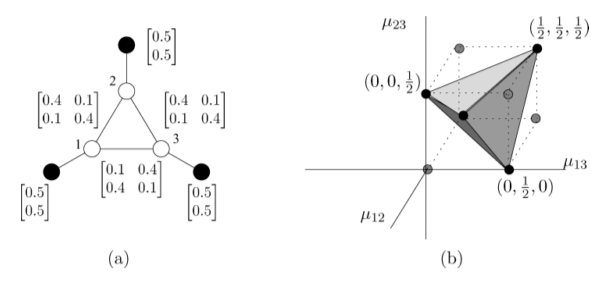
\includegraphics[width=.9\linewidth]{figure/4-1.PNG}
    \caption{
        (a) 特定的伪边际:将式 (4.9) 参数设置为 $\beta_{12} = \beta_{23} = 0.4, \beta_{13} = 0.1$,该伪边际满足局部一致性,不满足全局一致性。
        (b) 三点环图的边际多面体 $\mathbb{M}(C_3)$;
    }\label{fig:4-1}
\end{figure}

\subsection{贝特近似熵}

现在我们转向 Sum-product 算法的第二个变分成分,即对偶函数(负熵)的近似。
与边际多面体的外界 $\mathbb{L}(G)$ 一样,Bethe 熵近似也是基于树结构导出的。

对于一般的带环图上的 MRF 来说,负熵 $A^*$ —— 一个仅仅定义在均值参数 $\mu$ 上的函数 —— 明显缺乏封闭形式的表达式。
这种现象的一个重要例外是树结构上的 MRF,其熵可以分解为图上节点和边的局部熵。
为了导出这种分解形式,参考命题 4.1 的证明中因子分解式 (4.8),它将任意树结构的 MRF 分布分解为树上节点跟连边的边际分布 $\{\mu_s, s \in V\}$ 和 $\{\mu_{st}, (s, t) \in E\}$。
这些边际分布对应于正则过完备充分统计量 (3.34) 下的均值参数。
因此,对于树结构的 MRF,我们也能直接计算(负)对偶值 $-A^*(\mu)$,只需要计算分布 (4.8) 对应的熵 $H(p_{\mu})$ 即可。
使用 $\mathbb{E}_{\mu}$ 表示分布 (4.8) 下的期望,有:
\begin{align}
    H(p_{\mu}) = -A^*(\mu) &= \mathbb{E}_{\mu}[-\log p_{\mu}(X)] \nonumber \\
    &= \sum_{s \in V}H_s(\mu_s) - \sum_{(s, t) \in E}I_{st}(\mu_{st})
\end{align}
式中每个节点 $s \in V$ Singleton 的熵:
\begin{equation}
    H_s(\mu_s) := -\sum_{x_s \in \mathcal{X}_s}\mu_s(x_s)\log\mu_s(x_s)
\end{equation}
每条边 $(s, t) \in E$ 的互信息:
\begin{equation}
    I_{st}(\mu_{st}) := \sum_{(x_s, x_t) \in \mathcal{X}_s \times \mathcal{X}_t} \mu_{st}(x_s, x_t)\log\frac{\mu_{st}(xs, xt)}{\mu_s(x_s)\mu_t(x_t)}
\end{equation}
因此,对于树结构的图来说,对偶函数 $A^*$ 能够表达为一种精确且容易计算的均值参数 $\mu$ 的函数形式。

有了以上背景,带环图 MRF 的熵的 Bethe 近似就很容易描述了:
它简单地假定分解式 (4.11) 是带环图的一个合理近似。
根据这个假设,Bethe 近似熵可以表示为:
\begin{equation}
    -A^*(\mu) \approx H_{Bethe}(\tau) := \sum_{s \in V}H_s(\tau_s) - \sum_{(s, t) \in E}I_{st}(\tau_{st}).
\end{equation}
近似 (4.14) 可以用于任何一组属于 $\mathbb{L}(G)$ 的伪边际 $\{\tau_s, s \in V\}$ 以及 $\{\tau_{st}, (s, t) \in E\}$,这是 Sum-product 算法推导的核心条件。
因此,我们在符号上有意地将表示精确边际的 $\mu$ 换到了表示伪边际的 $\tau$。

Yedidia et al. 曾使用过一种不同于式 (4.14) 的 Bethe 近似熵,其实质是将互信息展开:$I_{st}(\tau_{st}) = H_s(\tau_s) + H_t(\tau_t) - H_{st}(\tau_{st})$,其中 $H_{st}$ 为伪边际 $\tau_{st}$ 的联合熵。
运用上述代换再经过简单的代数运算可得:
\begin{equation}
    H_{Bethe}(\tau) = -\sum_{s \in V}(d_s-1)H_s(\tau_s) + \sum_{(s, t) \in E}H_{st}(\tau_{st}), 
\end{equation}
式中 $d_s$ 代表节点 $s$ 的邻居数目(也就是节点 $s$ 的度)。
但是,对称形式的 (4.14) 在后续推断中是最自然的。

\subsection{贝特变分问题与和积算法}

我们现在已经具备了从定理 3.4 中的变分原理 (3.45) 中构建 Bethe 近似的两个原材料:
\begin{itemize}
    \item 满足局部一致性的伪边际 (4.7) 集合 $\mathbb{L}(G)$,其作为边际多面体 $\mathbb{M}(G)$ 的凸多面体外界;
    \item Bethe 熵 (4.14),其作为精确对偶函数 $A^*(\tau)$ 的近似。
\end{itemize}
组合两者即可得到 Bethe 变分问题(Bethe Variational Problem,BVP):
\begin{equation}
    \max_{\tau \in \mathbb{L}(G)}\left\{\langle\theta, \tau\rangle + \sum_{s \in V}H_s(\tau_s) - \sum_{(s, t) \in E}I_{st}(\tau_{st})\right\}.
\end{equation}

应当指出的是,这个问题具有一个非常简单的结构:
成本函数是显式给出的并且可微,约束集合 $\mathbb{L}(G)$ 是一个由少量约束决定的多面体。
给定这个特殊的结构,很容易想到优化问题 (4.16) 会有一个相对简单的求解算法,Sum-product 算法就是其中之一。

为了给出变分问题 (4.16) 与 Sum-product 算法之间的联系,令 $\lambda_{ss}$ 为归一化约束 $C_{ss}(\tau) = 0$ 的 Lagrange 乘子,其中:
\begin{equation}
    C_{ss}(\tau) := 1 - \sum_{x_s}\tau_s(x_s)
\end{equation}
此外,对每条边的每个方向 $s \rightarrow s$ 以及每个状态 $x_s \in \mathcal{X}_s$,定义如下约束函数:
\begin{equation}
    C_{ts}(x_s; \tau) := \tau_s(x_s) - \sum_{x_t}\tau_{st}(x_s, x_t),
\end{equation}
并且令 $\lambda_{ts}(x_s)$ 为约束 $C_{ts}(x_s; \tau) = 0$ 的 Lagrange 乘子。
这些 Lagrange 乘子与 Sum-product 消息联系紧密,事实上有 $M_{ts}(x_s) \propto \exp(\lambda_{ts}(x_s))$。

接下来考虑 Bethe 变分问题 (4.16) 的 Lagrangian:
\begin{align}
    \mathcal{L}(\tau, \lambda; \theta) := &\langle\theta, \tau\rangle + H_{Bethe}(\tau) + \sum_{s \in V}\lambda_{ss}C_{ss}(\tau) \nonumber \\
    & + \sum_{(s, t) \in E}\left[\sum_{x_s}\lambda_{ts}(x_s)C_{ts}(x_s; \tau) + \sum_{x_t}\lambda_{st}(x_t)C_{st}(x_t; \tau)\right].
\end{align}
依据上述定义,Yedidia et al. 给出了 Sum-product 算法与 BVP 的精确关系:

\begin{tcolorbox}
\begin{prop}[Sum-product 算法与 Bethe 问题]
    Sum-product 的消息更新机制是解决 Bethe 变分问题的一种 Lagrangian 方法:
    \begin{itemize}
        \item[(a)] 对于任意图 $G$,Sum-product 算法得到的任何不动点都给出一对 $(\tau^*, \lambda^*)$ 满足:
            \begin{equation}
                \nabla_{\tau}\mathcal{L}(\tau^*, \lambda^*; \theta) = 0, \quad \nabla_{\lambda}\mathcal{L}(\tau^*, \lambda^*; \theta) = 0.
            \end{equation}
        \item[(b)] 对于树结构的 MRF,Lagrangian 方程 (4.20) 有且仅有一个解 $(\tau^*, \lambda^*)$,其中 $\tau^*$ 的元素符合 MRF 精确的 Singleton 与 Pairwise 边际分布。
            此外,BVP 的最优值等价于累积函数 $A(\theta)$。
    \end{itemize}
\end{prop}
\end{tcolorbox}

\begin{tcolorbox}
\textbf{引注 4.1} 
    应当指出的是 Lagrangian 公式 (4.19) 是有所保留的,因为它只为归一化约束 $C_{ss}$ 与边际约束 $C_{ts}$ 配置了 Lagrange 乘子,而对非负性约束则采取了隐式处理。
    然而根据命题 4.2(a),Bethe 变分问题的任何严格正的最优解 $\tau^*$ 都必须满足 Lagrangian 条件 (4.20)。
    根据 Bertsekas 的工作,如果 $\lambda^*$ 是 BVP 的 Lagrange 乘子向量,那么最优解 $\tau^*$ 一定在正象限 $\tau \geq 0$ 最大化 Lagrangian $\mathcal{L}(\tau, \lambda^*)$。
    如果最优解 $\tau^*$ 严格正,那么 Lagrangian 最优性的一个必要条件就是 0 梯度条件 $\nabla_{\tau}\mathcal{L}(\tau^*, \lambda^*) = 0$。
    此外,对于为任意状态都分配了严格正质量的图模型(例如有限 $\theta$ 指数族形式的图模型)而言,Sm-product 算法传递的“消息”严格大于 0,因此也一定存在一个严格正的最优解 $\tau^*$。
    在这种情况下,命题 4.2(a) 保证了任意满足 Lagrangian 条件的 Sum-product 不动点都是 Bethe 变分问题的最优解。
    对于具有部分 0 质量状态的图模型而言则需要考虑另外的条件来保证不动点的最优性;
    详情可参见 Yedudua et al. 的工作。
\end{tcolorbox}

\analysis[证明]
(a) 部分的证明:计算偏导数 $\nabla_{\tau}\mathcal{L}(\tau; \lambda)$ 并让它等于 0 可得:
\begin{subequations}
\begin{align}
    \log\tau_s(x_s) &= \lambda_{ss} + \theta_s(x_s) + \sum_{t \in N(s)}\lambda_{ts}(x_s), \\
    \log\frac{\tau_{st}(x_s, x_t)}{\tilde{\tau}_s(x_s)\tilde{\tau}_t(x_t)} &= \theta_{st}(x_s, x_t) - \lambda_{ts}(x_s) - \lambda_{st}(x_t), 
\end{align}
\end{subequations}
其中 $\tilde{\tau}_s(x_s) := \sum_{x_t}\tau(x_s, x_t)$。
条件 $\nabla_{\lambda}\mathcal{L}(\tau; \lambda) = 0$ 等价于 $C_{ts}(x_s; \tau) = 0$ 以及 $C_{ss}(\tau) = 0$。
利用式 (4.21a) 以及边际条件 $C_{ts}(x_s; \tau) = 0$ 将式 (4.21b) 改写为:
\begin{align}
    \log\tau_{st}(x_s, x_t) &= \lambda_{ss} + \lambda_{tt} + \theta_{st}(x_s, x_t) + \theta_s(x_s) + \theta_t(x_t) \nonumber \\
    & + \sum_{u \in N(s)/t}\lambda_{us}(x_s) + \sum_{u \in N(t)/s}\lambda_{ut}(x_t).
\end{align}
为了建立与 Sum-product 算法的准确联系,我们为每条有向边 $t \rightarrow s$ 定义一个 $r_s$ 维的“消息”向量
\begin{equation*}
    M_{ts}(x_s) = \exp(\lambda_{ts}(x_s)), \quad \forall x_s \in \{0, 1, \cdots, r_s-1\}
\end{equation*}
使用这种记号式 (4.21a) 可以改写为:
\begin{equation}
    \tau_s(x_s) = \kappa\exp(\theta_s(x_s))\prod_{t \in N(s)}M_{ts}(x_s).
\end{equation}
式 (4.22) 可以改写为:
\begin{align}
    \tau_{st}(x_s, x_t) &= \kappa'\exp(\theta_{st}(x_s, x_t) + \theta_s(x_s) + \theta_t(x_t)) \nonumber \\
    &= \times \prod_{u \in N(s)/t}M_{us}(x_s) \prod_{u \in N(t)/s}M_{ut}(x_t).
\end{align}
式中 $\kappa, \kappa'$ 是依赖于 $\lambda_{ss}, \lambda_{tt}$ 的正常数,用于保证伪边际的归一化条件。
注意 $\tau_s$ 以及 $\tau_{st}$ 被定义为非负的。

综上,我们需要调整 Lagrange 乘子或者消息以使得每条边都满足边际约束 $\sum_{x_t}\tau_{st}(x_s, x_t) = \tau_s(x_s)$。
根据式 (4.23) 和 (4.24) 可得:
\begin{equation}
    M_{ts}(x_s) \propto \sum_{x_t}\left[\exp\{\theta_{st}(x_s, x_t)+\theta_t(x_t)\}\prod_{u \in N(t)/s}M_{ut}(x_t)\right], 
\end{equation}
上式与 Sum-product 的更新式 (2.9) 等价。
通过上述构造可以证明,式 (4.25) 更新得到的任何不动点 $M^*$ 都确定了一对 $(\tau^*, \lambda^*)$ 满足驻点条件 (4.20)。

\begin{note}
    译者经过计算给出的关系式与 (4.21) 不同:
    \begin{align*}
        \frac{\partial \mathcal{L}}{\partial \tau_s(x_s)} &= \theta_s(x_s) - \log\tau_s(x_s) - \lambda_{ss} + \sum_{t \in N(s)}\lambda_{ts}(x_s) \\
        &= 0 \\
        \Rightarrow \log\tau_{s}(x_s) &= \theta_s(x_s) - \lambda_{ss} + \sum_{t \in N(s)}\lambda_{ts}(x_s) \\
        \frac{\partial \mathcal{L}}{\partial \tau_{st}(x_s, x_t)} &= \theta_{st}(x_s, x_t) - \log\frac{\tau_{st}(x_s, x_t)}{\tau_s(x_s)\tau_t(x_t)} - 1 - \lambda_{ts}(x_s) - \lambda_{st}(x_t) \\
        &= 0 \\
        \Rightarrow \log\frac{\tau_{st}(x_s, x_t)}{\tau_s(x_s)\tau_t(x_t)} &= \theta_{st}(x_s, x_t) -1 - \lambda_{ts}(x_s) - \lambda_{st}(x_t)
    \end{align*}
    因此,式 (4.22) 也有不同:
    \begin{align*}
        \log\tau_{st}(x_s, x_t) &= -1 - \lambda_{ss} - \lambda_{tt} + \theta_{st}(x_s, x_t) + \theta_s(x_s) + \theta_t(x_t) \\
        & + \sum_{u \in N(s)/t}\lambda_{us}(x_s) + \sum_{u \in N(t)/s}\lambda_{ut}(x_t).
    \end{align*}
    然而在后续推导中这些问题均隐含在归一化常数 $\kappa$ 与 $\kappa'$ 里,因此形式上的差异消失了。
\end{note}

(b) 部分的证明参见附录 B.4。
\qed

Sum-product 算法与 Bethe 变分原理之间的这种联系可以导出许多重要结论。
首先,它为在带环图上应用 Sum-product 算法提供了理论基础,也就是采用一种迭代的方式尝试解出满足 Lagrangian 条件的解。
然而应当注意的是,Sum-product 与 Bethe 问题之间的这种联系并未保证 Sum-product 迭代可以在带环图上收敛。
实际上,算法能否收敛取决于势强度(Potential Strengths)以及图的拓扑结构。
标准的消息传递机制中,每个节点都是并行应用式 (4.25) 的。
其他更为全局性的消息传递机制也是可行的,这些机制也可以用在例如纠错编码等特定应用中。
Tatikonda 和 Jordan 在无限展开的计算树(Infinitely Unwrapped Computation Tree)上建立了并行更新的收敛条件和 Gibbs 测度之间的联系,从而表明了由 Gibbs 测度的经典唯一性条件可以得到收敛的充分条件(也就是 Dobrushin 条件或者 Simon 条件)。
在之后的工作中,其他研究人员使用了各种类型的收缩论点来获得更清晰的不动点的收敛条件和唯一性条件。
对于某种程度的弱势(Suitably Weak Potentials),Dobrushin 条件和相关的压缩参数可以保证更新的收敛性,也就保证了相关不动点的唯一性。
另一些工作也在探索 Sum-product 的替代方案,这些方案可以保证收敛,只不过需要增加计算成本。
但是,除了树和某些特殊情况,Bethe 变分问题通常是非凸的,因为 $H_{Bethe}$ 并不是凹的。
因此即使使用了收敛算法也不能保证收敛到全局最优值,经常会收敛到局部最优。

对于每个 $\theta \in \mathbb{R}^d$,令 $A_{Bethe}(\theta)$ 代表 Bethe 变分问题 (4.16) 的最优值。
命题 4.2(b) 表明对于任意的树结构问题,有 $A_{Bethe}(\theta) = A(\theta)$,这个等式对所有 $\theta \in \mathbb{R}^d$ 成立。
在这种等价性下很容易自然联想到对于一般图来说 $A_{Bethe}(\theta)$ 和累积函数 $A(\theta)$ 之间的关系。
一般而言,Bethe 值 $A_{Bethe}(\theta)$ 只是累积函数 $A(\theta)$ 的一个简单近似。
与第 5 节会讨论的平均场方法不同,$A_{Bethe}(\theta)$ 并不保证是累积函数的一个下界。
第 7 节中将会花费更长的篇幅来讨论由 Wainwright et al. 导出的 Convexified 形式的 Bethe 变分原理,它可以为任意图模型提供关于累积函数上界的估计。
另一方面,Sudderth et al. 发现对于某些有意思的图模型来说 $A_{Bethe}(\theta)$ 也确实是累积函数 $A(\theta)$ 的一个下界。
这些模型一般都鼓励随机变量彼此之间趋于一致,在计算机视觉与空间统计等应用中比较常见。
相应的下界性质跟 Bethe 近似与循环级数展开(Loop Series Expansions)之间的联系关系密切,4.1.6 小节将会对这一点进行讨论。

Bethe 问题与 Sum-product 算法之间的联系所导出的另一个重要结论是,通过逐步更好地逼近熵函数和边际多面体的外边界可以提出许多改进普通 Sum-product 算法的方法。
4.2 节将会讨论一类这样的广义 Sum-product 算法。

\subsection{贝特问题与和积算法的误差}

这一小节我们讨论 Sum-product 算法的误差。
从变分的角度来看,误差来源于构造 Bethe 变分原理的两个近似:

\begin{itemize}
    \item[(1)] 采用多面体外界 $\mathbb{L}(G)$ 代替了边际多面体 $\mathbb{M}(G)$,
    \item[(2)] 采用 Bethe 熵 $H_{Bethe}$ 作为均值参数精确熵函数的近似。
\end{itemize}

我们先考虑 Bethe 熵近似以及它带来的潜在误差:

\begin{tcolorbox}
\begin{exam}[$H_{Bethe}$ 的误差]

考虑四个节点的全连接图 $K_4$,Singleton 与 Pairwise 的边际分布为:
\begin{subequations}
\begin{align}
    \mu_s(x_s) &= [0.5, 0.5] &\text{for } s = 1, 2, 3, 4 \\
    \mu_{st}(x_s, x_t) &= \begin{bmatrix}
        0.5 & 0 \\
        0 & 0.5
    \end{bmatrix} &\forall (s, t) \in E.
\end{align}
\end{subequations}
这些边际满足全局一致性,事实上,在状态 $(0, 0, 0, 0)$ 与 $(1, 1, 1, 1)$ 上各自分配 0.5 的概率就可以导出这些边际。
Bethe 近似熵的计算很简单,每个 Singleton 的熵为 $H_s(\mu_s) = \log 2$,每条边的互信息为 $I_{st}(\mu_{st}) = \log 2$,所以 Bethe 熵为:
\begin{equation*}
    H_{Bethe}(\mu) = 4\log 2 - 6\log 2 = -2\log 2 < 0,
\end{equation*}
显然不可能是一个真正的熵值。
事实上,这个例子的真熵值(或者说负对偶函数值)为 $-A^*(\mu) = \log 2 > 0$。

\end{exam}
\end{tcolorbox}

除了采用 $H_{Bethe}$ 作为负对偶函数的近似之外,Bethe 变分原理的误差还来自于将边际多面体 $\mathbb{M}(G)$ 放松到了一阶约束集合 $\mathbb{L}(G)$ 上。
如例 4.1 所示,3 个节点的环 $C_3$ 严格满足包含关系 $\mathbb{M}(C_3) \subseteq \mathbb{L}(C_3)$。
将例 4.1 的构造方法进行拓展可以证明包含关系 $\mathbb{M}(G) \subset \mathbb{L}$ 对于任何带环图 $G$ 都是严格成立的。
图 \ref{fig:4-2} 给出了 $\mathbb{M}(G)$ 和 $\mathbb{L}(G)$ 之间关系的一个理想化的示意图\footnote{
    应当指出的是这幅图也具有一定的误导性,因为在那上面 $\mathbb{L}(G)$ 比 $\mathbb{M}(G)$ 具有更多的切面和顶点。
    事实上多面体 $\mathbb{L}(G)$ 的切面数目更少而顶点数目更多,但这种特性在二维图上很难表示出来。
}:两个集合都是多面体,同时对于任意带环图来说,$\mathbb{M}(G)$ 总是严格含于外边界 $\mathbb{L}(G)$。

\begin{figure}[htbp]
    \centering
    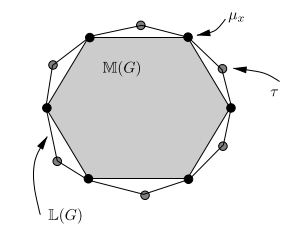
\includegraphics[width=.5\linewidth]{figure/4-2.PNG}
    \caption{
        边际多面体 $\mathbb{M}(G)$ 与外边界 $\mathbb{L}(G)$ 之间关系的理想化示意图。
        集合 $\mathbb{L}(G)$ 永远是 $\mathbb{M}(G)$ 的一个外边界,而对于任意带环图 $G$ 来说包含关系 $\mathbb{M}(G) \subset \mathbb{L}(G)$ 都严格成立。
        两个集合都是多面体,所以都能够用有限数目的极值点(Extreme Points)构成的凸包(Convex Hull)或者有限数目的半空间(Half-spaces)也就是切面(Facets)进行表示。
    }\label{fig:4-2}
\end{figure}

这两个集合都是多面体,因此可以表示为有限数目的极值点的凸包,或者是有限数目的半空间也就是切面的交集。
令 $\phi$ 代表标准过完备表示 (3.34) 指示函数所构成的全向量,边际多面体可以表示为凸包 $\mathbb{M}(G) = conv\{\phi(x)| x \in \mathcal{X}^m\}$。
由于指示函数为 $\{0, 1\}$ 取值,它的所有极值点都是由 $\{0, 1\}$ 元素构成,其实质为某些 $x \in \mathcal{X}^m$ 的特征量 $\mu_x := \phi(x)$,这样的极值点一共有 $|\mathcal{X}^m|$ 个。
然而除了树结构的图之外,$\mathbb{M}(G)$ 切面的数目一般是未知的,对于简单如 Ising 模型等例子也是如此。
而且切面的数目随着图的规模的增长一定是超多项式的(Super-polynomial),除非在计算复杂度方面某些被广泛认可的猜想实际是错的。

另一方面,多面体 $\mathbb{L}(G)$ 具有多项式数目的切面,对于任意图模型来说都有上界 $\mathcal{O}(rm+r^2|E|)$。
$\mathbb{L}(G)$ 相比 $\mathbb{M}(G)$ 具有更多的极值点,因为除了所有的整点(Integral Extreme Points)$\{\mu_x, x \in \mathcal{X}^m\}$ 之外,它还包括其他一些具有分数元素的极值点 $\tau \in \mathbb{L}(G)/\mathbb{M}(G)$。
8.4 节对整数极值点和分数极值点进行了进一步的讨论。
除了树和其他一些小规模的实例外,$\mathbb{L}(G)$ 的极值点数目一般也是未知的。

$\mathbb{M}(G)$ 与 $\mathbb{L}(G)$ 之间的严格包含关系 —— 以及后者在 Bethe 变分问题 (4.16) 中的基本角色 —— 引出了以下问题:
Bethe 变分问题的解会总是落入 $\mathbb{M}(G)/\mathbb{L}(G)$ 的间隔(Gap)中吗?
乐观主义者会希望这些点能通过某种方式被排除在 Bethe 变分问题的最优解之外。
不幸的是,这种乐观主义想法被证明是具有误导性的。
事实上,对于 $\mathbb{L}(G)$ 中的每一个元素 $\tau$ 都可以构造一个分布 $p_{\theta}$,使得 $\tau$ 满足 Sum-product 的不动点所定义的消息。
为了理解这件事情,我们接下来讨论 Sum-product 的重参数化解释(Reparameterization Interpretation)。

\subsection{贝特最优与重参数化}

2.5.2 小节描述的联合树算法可以从如下角度进行理解:
将某个图上团的势函数集合作为输入,联合树算法输出相同分布的因子分解结果,这些因子就是联合树上的团集和分割集上的局部边际。
在树结构的特殊情况下,因子是各个节点以及各个连边上的边际,如式 (4.8) 所示。
事实上,树的 Sum-product 算法可以被理解为进行这种参数化的有效方法。

同样的解释也适用于任意带环图:
更准确地说,Sum-product 算法的任何不动点 —— 甚至更普遍地说,Bethe 变分原理的任意局部最优点 —— 都指定了原始分布 $p_{\theta}$ 的一种重参数化形式。
我们将这一事实总结为如下命题:

\begin{tcolorbox}
\begin{prop}[Bethe 近似的重参数化性质]

令 $\tau^* = (\tau_s^*, s \in V; \tau_{st}^*, (s, t) \in E)$ 表示由分布 $p_{\theta}$ 定义的 Bethe 变分原理的任意最优点。
则根据该不动点定义的如下分布:
\begin{equation}
    p_{\tau^*}(x) := \frac{1}{Z(\tau^*)}\prod_{s \in V}\tau_s^*(x_s)\prod_{(s, t) \in E}\frac{\tau_{st}^*(x_s, x_t)}{\tau_s^*(x_s)\tau_t^*(x_t)},
\end{equation}
就是原始分布 $p_{\theta}$ 的一种重参数化形式 —— 也就是说对于所有 $x \in \mathcal{X}^m$,都有 $p_{\tau^*}(x) = p_{\theta}(x)$。

\end{prop}
\end{tcolorbox}

应当注意的是,这种重参数化仅仅在由指示函数 (3.34) 定义的过完备表示下的指数族中有效。
重参数化 (4.27) 实际上是树结构分解 (4.8) 的一个类比,只不过应用在带环图上。
与树结构情况不同的是,归一化常数 $Z(\tau^*)$ 一般并不等于 1。
尽管联合树定理保证了任何树结构可以进行重参数化,但是对于一般的图而言,即使重参数化存在也是不容易直接看出来的。
事实上,每个图至少有一个这种形式的重参数化表示,有些图可能有多个,例如对于任何 BVP 具有多个最优解的问题就是如此。
此外,重参数化观点为 $p_{\theta}(x)$ 的精确边际 $\mu_s$ 与由 Sum-product 算法给出的近似 $\tau_s^*$ 之间的差异 所造成的近似误差提供了一些见解。
实际上,应用式 (4.27) 可以推导出 Sum-product 算法中的误差的精确表达式,以及可计算的误差界,这些工作由 Wainwright et al. 完成。

我们接下来借助重参数化表征 (4.27) 为 $\mathbb{L}(G)$ 中的任何由 Sum-product 算法得到的不动点对应的伪边际 $\tau$ 指定相应的分布 $p_{\theta}$。
以下面这个例子进行说明。

\begin{tcolorbox}
\begin{exam}[“戏弄” Sum-product 算法]

我们还是考虑使 Sum-product 算法不精确的最简单的图,也就是三个节点的环(同例 4.1)。
考虑候选边际分布 $(\tau_s, s \in V)$ 以及 $(\tau_{st}, (s, t) \in E)$,并按图 \ref{fig:4-1}(a) 进行配置,$\beta_{12} = \beta_{23} = 0.4, \beta_{13} = 0.1$。
如例 4.1 中的讨论,这种配置所构建的伪边际 $\tau$ 是 $\mathbb{L}(G)$ 中的元素,但不是 $\mathbb{M}(G)$ 中的元素,因此也就无法从任何满足全局一致性的分布中导出。

现在让我们证明,对于图上一个经过适当选择的分布 $p_{\theta}$,Sum-product 算法是如何被“戏弄”从而收敛到伪边际向量 $\tau$ 上的。
使用正则过完备表示 (3.34),考虑如下形式的正则参数:
\begin{subequations}
\begin{align}
    \theta_s(x_s) &:= \log\tau_s(x_s) = \log [0.5, 0.5] &\forall s \in V, \\
    \theta_{st}(x_s, x_t) &:= \log\frac{\tau_{st}(x_s, x_t)}{\tau_s(x_s)\tau_t(x_t)} & \nonumber \\
    &= \log 4\begin{bmatrix}
        \beta_{st} & 0.5-\beta_{st} \\
        0.5-\beta_{st} & \beta_{st}
    \end{bmatrix} &\forall (s, t) \in E
\end{align}
\end{subequations}
式中我们采用了式 (4.2) 的简写。
在上面这些正则参数的配置下,假设我们在 MRF $p_{\theta}(x)$ 上应用 Sum-product 算法,并进行均匀初始化 $M_{ts}(x_s) \propto [0.5, 0.5]$。
根据式 (4.25) 可知,这种均匀初始化 $M$ 已经为 Sum-product 定义了一个不动点。
此外,如果我们计算由 $M$ 和 $\theta$ 指定的相应伪边际,就会发现结果就是之前定义的 $\tau_s$ 以及 $\tau_{st}$。
综上,当 Sum-product 算法应用于由式 (4.28) 所定义的正则参数相应的分布 $p_{\theta}$ 上时,会输出伪边际 $\tau$ 作为真实边际的估计。

读者可能会反对这样的初始化方法,也就是一开始就将消息初始化在不动点上会导致算法排除其他可能的不动点。
然而根据已有的一些工作,对于任何最多只有一个环路的离散指数族 MRF 来说,Sum-product 具有唯一的不动点,且一定收敛到该不动点。
因此,我们构造的不动点 (4.28) 是这个问题的唯一不动点,算法从消息的任意初始化开始都会收敛到这个不动点上。

\end{exam}
\end{tcolorbox}

更一般的说,上述例子中展示的构造方法适用于 $\mathbb{L}(G)$ 中的任何内点\footnote{
    严格说来,它适用于相对内部的元素,因为如过完备表示 (3.34) 所述,集合 $\mathbb{L}(G)$ 不是全维度的(Full-dimensional),因此有一个空的内部(Empty Interior)。
}。因此,对于所有的伪边际 $\tau \in \mathbb{L}(G)$,包括那些不满足全局一致性的,都存在分布 $p_{\theta}$ 可以使得 $\tau$ 从 Sum-product 的不动点中导出。

\begin{note}
    译者对脚注 (4) 产生了莫大的疑问。
    $\mathbb{L}(G)$ 为什么会有个“空的内部”?
    它不是一个简单的“实心”的凸多面体吗?
\end{note}

\subsection{贝特与循环级数展开}

本小节我们讨论 Chertkov 与 Chernyak 的循环级数展开。
这些展开项提供了累积函数作为项和的精确表示,其中第一项就是 Bethe 近似 $A_{Bethe}(\theta)$,并且可以通过添加所谓的循环修正(Loop Corrections)而得到高阶项。
他们为循环级数提供了两种推导:第一种对二元变量的 Fourier 表示应用了三角恒等式,第二种是通过复变量辅助场得到的鞍点近似。
在本小节中我们采用一种更为直接的方式来导出循环级数,这种方法利用了命题 4.3 中给出的 Sum-product 不动点的重参数化特征。
尽管循环级数展开可以扩展到一般的因子图上,但考虑带有二元变量的成对 MRF —— 即例 3.1 中的 Ising 模型 —— 足以说明基本思想。
(因子图的推导可以参见 Sudderth et al. 的工作。)

在揭示结论之前,我们先做一些初步的定义。
给定一个无向图 $G = (V, E)$ 以及连边 $E$ 的一个子集 $\tilde{E} \subseteq E$,令 $G(\tilde{E})$ 表示与连边集合 $\tilde{E}$ 与节点集合
\begin{equation}
    V(\tilde{E}) := \{t \in V| (t, u) \in \tilde{E} \quad \text{for some } u\}
\end{equation}
的一个子图。
对于任意节点 $s \in V$,我们定义其与 $\tilde{E}$ 相关的度为
\begin{equation}
    d_s(\tilde{E}) := \{t \in V| (s, t) \in \tilde{E}\}.
\end{equation}
根据 Chertkov 与 Chernyak 的工作,我们定义广义环(Generalized Loop)的概念为一个子图 $G(\tilde{E})$,其每个节点 $s \in V$ 的度均满足 $d_s(\tilde{E}) \neq 1$。
换句话说,对于每个节点 $s \in V$,它要么 $d_s(\tilde{E}) = 0$ 从而不属于 $G(\tilde{E})$,要么 $d_s(\tilde{E}) \geq 2$。
图 \ref{fig:4-3} 给出了广义环的示意说明。
应当指出的是,无环图(也就是树或者森林图)是没有任何广义环的。

\begin{figure}[htbp]
    \centering
    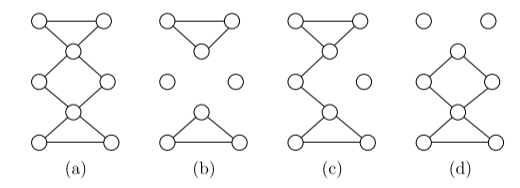
\includegraphics[width=.9\linewidth]{figure/4-3.PNG}
    \caption{
        广义环示意。
        (a) 原始图。
        (b)-(d) 与 (a) 中原始图相关的几个广义环。
        在这个特定的例子中,原始图自身也是一个自己的广义环。
    }\label{fig:4-3}
\end{figure}

考虑二元变量的成对 MRF —— 也就是 Ising 模型 (3.8) —— 的一个 BP 不动点。
对于二元变量 $X_s \in \{0, 1\}$,与 BP 不动点相关的 Singleton 和 Edgewise 的伪边际可以参数化为
\begin{equation}
    \tau_s(x_s) = \begin{bmatrix}
        1 - \tau_s \\
        \tau_s
    \end{bmatrix}, \quad \tau_{st}(x_s, x_t) = \begin{bmatrix}
        1 - \tau_s - \tau_t + \tau_{st} & \tau_t - \tau_{st} \\
        \tau_s - \tau_{st} & \tau_{st}
    \end{bmatrix}
\end{equation}
通过一些简单的计算可以将 $\mathbb{L}(G)$ 用以下四个不等式进行描述:
\begin{equation*}
    \tau_{st} \geq 0, 1-\tau_s-\tau_t+\tau_{st} \geq 0, \tau_s-\tau_{st} \geq 0, \tau_t-\tau_{st} \geq 0,
\end{equation*}
这四个不等式对每条边 $(s, t) \in E$ 都成立。
有关 Ising 模型的均值参数的讨论可以参见例 3.8。

使用这个参数表示,我们为每条边 $(s, t) \in E$ 定义边权重(Edge Weight)
\begin{equation}
    \beta_{st} := \frac{\tau_{st}-\tau_s\tau_t}{\tau_s(1-\tau_s)\tau_t(1-\tau_t)}
\end{equation}
将其自然拓展到子图权重(Subgraph Weight)$\beta_{\tilde{E}} := \prod_{(s, t) \in \tilde{E}}\beta_{st}$。
有了这些定义,我们可以提出以下命题:

\begin{tcolorbox}
\begin{prop}

考虑一个二元变量的成对 MRF (3.8),令 $A_{Bethe}(\theta)$ 表示自由能 (4.16) 在 BP 不动点 $\tau = (\tau_s, s \in V; \tau_{st}, (s, t) \in E)$ 处取得的最优值。
累积函数 $A(\theta)$ 等价于下列循环级数展开:
\begin{equation}
    A(\theta) = A_{Bethe}(\theta) + \log\left\{1+\sum_{\emptyset\neq\tilde{E}\subseteq E}\beta_{\tilde{E}}\prod_{s \in V}\mathbb{E}_{\tau_s}[(X_s - \tau_s)^{d_s(\tilde{E})}]\right\}.
\end{equation}

\end{prop}
\end{tcolorbox}

在证明命题 4.4 之前,我们先暂停一下做一些注释。
根据定义我们有
\begin{align}
    \mathbb{E}_{\tau_s}[(X_s - \tau_s)^d] &= (1-\tau_s)(-\tau_s)^d + \tau_s(1-\tau_s)^d \nonumber \\
    &= \tau_s(1-\tau_s)[(1-\tau_s)^{d-1}+(-1)^d(\tau_s)^{d-1}], 
\end{align}
其实质是一个参数为 $\tau_s \in [0, 1]$ 的 Bernoulli 变量的 $d$ 阶中心矩。
因此,对于至少有一个节点 $s \in V$ 满足 $d_s(\tilde{E}) = 1$ 的连边子集 $\tilde{E} \subseteq E$,其在展开式 (4.33) 中相应的项被消除了。
所以,只有广义环 $\tilde{E}$ 在展开式 (4.33) 中保留下来。
与这些广义环相关的项定义了对累积函数的 Bethe 近似 $A_{Bethe}(\theta)$ 的修正。
此外,树结构的图不包含任何非平凡的广义环,这提供了树结构图的 Bethe 近似实际上十分精确的另一种证明。

循环展开的第一项 $A_{Bethe}(\theta)$ 很容易从任何 BP 不动点计算出来,因为它只对应于 Bethe 自由能的最优值 (4.16)。
然而,整个循环修正序列的显式计算 —— 也就是对累积函数的精确计算 —— 对于一般的图模型来说仍旧困难。
例如,任何 $n \geq 5$ 个节点的全连通图都有超过 $2^n$ 个广义环。
在某些情况下,对一小组重要的循环修正进行计算可能会提高对配分函数的近似,或者为 LDPC 编码的边际提供更加精确的近似。

\analysis[命题 4.4 的证明]
使用指示函数进行的正则过完备参数化 (3.34) 是过完备的,因此有许多不同的正则参数向量 $\theta \neq \theta'$ 对应相同的分布 $p_{\theta} = p_{\theta'}$。
然而,循环级数展开 (4.33) 左侧与右侧的区别对于任意 $\theta$ 都是相同的,因为变换 $\theta \rightarrow \theta'$ 仅仅将 $A(\theta)$ 与 $A_{Bethe}(\theta)$ 都偏移了同一个常数。
因此,我们只需要证明一种参数化形式的循环级数展开即可;
特别地,我们选择使用由任意 BP 不动点给出的重参数化形式下的正则参数:
\begin{equation}
    \tilde{\theta} = \log\tau_s(x_s), \quad \tilde{\theta}_{st}(x_s, x_t) = \log\frac{\tau_{st}(x_s, x_t)}{\tau_s(x_s)\tau_t(x_t)}.
\end{equation}
在这个重参数化形式下,通过简单计算即可知 $A_{Bethe}(\tilde{\theta}) = 0$。
因此,我们只需要证明在这个重参数化 (4.35) 条件下等式
\begin{equation}
    A(\tilde{\theta}) = \log\left\{1+\sum_{\emptyset\neq\tilde{E}\subseteq E}\beta_{\tilde{E}}\prod_{s \in V}\mathbb{E}_{\tau_s}[(X_s-\tau_s)^{d_s(\tilde{E})}]\right\}
\end{equation}
成立即可。
使用表示 (4.31),通过简单的计算可知
\begin{equation}
    \frac{\tau_{st}(x_s, x_t)}{\tau_s(x_s)\tau_t(x_t)} = 1 + \beta_{st}(x_s-\tau_s)(x_t-\tau_t).
\end{equation}
根据 $\tilde{\theta}$ 的定义,我们有
\begin{equation*}
    \exp(A(\tilde{\theta})) = \sum_{x \in \{0, 1\}^m}\prod_{s \in V}\tau_s(x_s)\prod_{(s, t) \in E}\frac{\tau_{st}(x_s, x_t)}{\tau_s(x_s)\tau_t(x_t)}.
\end{equation*}
令 $\mathbb{E}$ 表示乘积分布 $\tau_{fact}(x) := \prod_s\tau_s(x_s)$ 下的期望。
考虑 (4.37) 式,我们有
\begin{align}
    \exp(A(\tilde{\theta})) &= \sum_{x \in \{0, 1\}^m}\prod_{s \in V}\tau_s(x_s)\prod_{(s, t) \in E}\frac{\tau_{st}(x_s, x_t)}{\tau_s(x_s)\tau_t(x_t)} \nonumber \\
    &= \mathbb{E}\left[\prod_{(s, t) \in E}(1+\beta_{st}(X_s-\tau_s)(X_t-\tau_t))\right].
\end{align}
对这个多项式进行展开并利用期望的线性性质,可以得到图中每个非空的连边子集 $\tilde{E} \subseteq E$ 对应的项:
\begin{equation}
    \exp(A(\tilde{\theta})) = 1 + \sum_{\emptyset\neq\tilde{E}\subseteq E}\mathbb{E}\left[\prod_{(s, t) \in \tilde{E}}\beta_{st}(X_s-\tau_s)(X_t-\tau_t)\right].
\end{equation}
之后,表达式 (4.36) 可以依据 $\tau_{fact}(x)$ 的独立性与 Bernoulli 变量的矩的标准公式得到。
计算过程中应当注意如果 $d_s(\tilde{E}) = 1$,那么就有 $\mathbb{E}[X_s-\tau_s] = 0$。
因此,每个广义环 $\tilde{E}$ 都会有一个循环校正。
\qed

命题 4.4 可以拓展到更加一般的因子图上。
此外,Sudderth et al. 的工作表明对于一类具有相互吸引作用的图模型来说,其 Bethe 值 $A_{Betha}(\theta)$ 实际上是真实累积函数 $A(\theta)$ 值的一个下界。

\section{菊池与基于超树的方法}

Bethe 变分原理 (4.16) 从两种不同的角度对精确变分原理 (3.45) 进行了近似。
首先对于一般图而言,Bethe 熵 (4.14) 仅仅是真实熵或者说负对偶函数的近似。
其次约束集合 $\mathbb{L}(G)$ 也是边际多面体 $\mathbb{M}(G)$ 的一个外边界,如图 \ref{fig:4-2} 所示。
从原理上来说,Bethe 变分原理可以通过对两者进行改进来提升近似效果。
本节主要考虑一种自然的拓展方法来对 Bethe 近似进行泛化,这些工作最开始是由 Yedidia et al. 提出的,之后也得到了其他研究者的拓展,对 Bethe 近似的两个成分都进行了改进。
这些方法的原始记录来源于统计物理文献,被称为簇变分方法(Cluster Variational Methods)。

从高一点的视角来看,Bethe 方法给出的近似是基于树结构的,这是联合树结构的一种特例。
那么一种自然的拓展策略就是考虑对更加复杂的联合树进行近似。
这些近似条件在超树(Hypertrees)的结构上很容易理解,因为超树就是联合树的表示方法之一。
因此,接下来我们介绍一些超图(Hypergraphs)和超树的必要背景。

\subsection{超图和超树}

超图 $G = (V, E)$ 是对图的一种泛化,包括节点集合 $V = \{1, \cdots, m\}$,以及超边(Hyperedges)集合 $E$,所谓的超边 $h$ 是指节点集合 $V$ 的一个特定子集。
这些超边构成了一个偏序集(Partially Ordered Set,Poset),这种偏序性质是由包含关系给出的。
当一条超边 $h$ 不被其他超边包含的时候,则称该超边 $h$ 为最大的(Maximal)。
根据这些定义,我们可以看到普通图就是超图的特例,其中每个最大超边由一对顶点构成,也就是普通图的一条普通边\footnote{
    我们这里的超边集合 $E$ 的定义与图论术语有一个小小的不同,对于超图(不是普通图),超边集合可以包含一个单独的节点 $\{s\}$ 作为一个元素。
}。

超图中有一种方便的图表示方法,那就是用超边图来表示,也就是采用有向边来表示包含关系,这样的表示称为偏序集图(Poset Diagram)。
图 \ref{fig:4-4} 给出了一些简单的超图示例。
任何普通图,也就是超图的特例,也可以用偏序集图的方式画出来。
例如,子图 (a) 展示了四节点单环的超图表示,子图 (b) 展示了一个非普通图的超图,它由两个大小为 3 的超边以及大小为 2 的交集组成,子图 (c) 是一个更加复杂的超图,我们之后会继续讨论这个超图。

\begin{figure}[htbp]
    \centering
    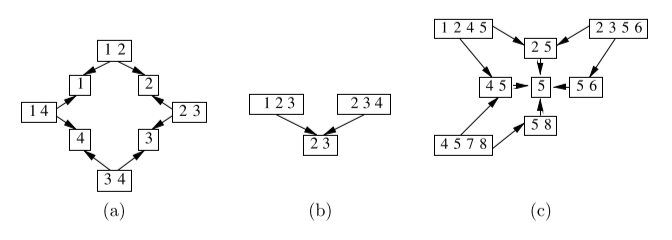
\includegraphics[width=.9\linewidth]{figure/4-4.PNG}
    \caption{
        超图的图表示。
        超边的节点子集用矩形表示,箭头则表示超边之间的包含关系。
        (a) 用超图表示的一个普通单环图。
        (b) 宽度为 2 的简单超树。
        (c) 宽度为 3 的一个更加复杂的超图。
    }\label{fig:4-4}
\end{figure}

超树,或者说无环超图,提供了一种方法来描述 2.5.2 小节中给出的联合树的概念。
特别地,如果超图可以使用最大超边和它们的交集给出一个联合树,那么这个超图就是无环的。
无环超图的宽度就是最大超边的大小减 1,我们将宽度为 $k$ 的由单个连通分量构成的无环超图称为 $k$ 阶超树(k-hypertree)。
例如,一个普通图的生成树是 1 阶超树,因为它的最大超边,也就是原始图中的一条普通边,大小都是 2。
再考虑图 \ref{fig:4-4}(c) 中的超图,显然这个超图等价于最大团为 $\{(1245), (4578), (2356)\}$,分割子为 $\{(25), (45)\}$ 的联合树。
因为最大超边的大小为 4,所以这个超图是一个宽度为 3 的超树。

\subsection{基于超树的因子化与熵的分解}

我们接下来给出联合树因子化 (2.12) 的另一种形式,并指出这种形式可以导致对熵的局部分解。
我们将超边集合 $E$ 看做是一个偏序集合,如附录 E.1 所描述的,每一个偏序集合都可以定一个 M\"obius 函数 $\omega: E \times E \rightarrow \mathbb{R}$。
使用边际集合 $\mu = (\mu_h, h \in E)$ 与超边集合进行关联,就能定义一个新的函数集合 $\varphi := (\varphi_h, h \in E)$ 如下:
\begin{equation}
    \log\varphi_h(x_h) := \sum_{g \subseteq h}\omega(g, h)\log\mu_g(x_g)
\end{equation}
根据以上定义以及 M\"obius 逆公式(参见附录 E.1 中的引理 E.1),边际可以表示为
\begin{equation}
    \log\mu_h(x_h) = \sum_{g \subseteq h}\log\varphi_g(x_g).
\end{equation}
这个公式为计算函数 $\varphi_g$ 提供了一种非常有用的递归方法,在下面会通过一个例子来进行说明。

函数 (4.40) 的意义在于为任何超树结构的图提供了一种非常简单的因子化方法。
特别地,对于具有包含最大超边之间交集的连边集合的超图来说,其上的分布具有如下因子分解:
\begin{equation}
    p_{\mu}(x) = \prod_{h \in E}\varphi_h(x_h; \mu)
\end{equation}
使用 $\varphi_h(x_h; \mu)$ 是为了强调 $\varphi_h$ 是边际 $\mu$ 的一个函数。
式 (4.42) 是著名的联合树分解 (2.12) 的另一种形式。
接下来我们通过一些例子加深理解。

\begin{tcolorbox}
\begin{exam}[超树的因子化]

(a) 首先假设超树为一个普通树,那么超边集合就是顶点集合与普通连边集合的并集。
将这个超边集合视为包含关系下的一个偏序集,那么其 M\:obius 函数具有如下形式:
对于所有超边 $g \in E$,有 $\omega(g, g) = 1$;
对于所有顶点 $s$ 以及普通连边 $\{s, t\}$,有 $\omega(\{s\}, \{s, t\}) = -1$;
另外对于所有不含于 $h$ 的 $g$,有 $\omega(g, h) = 0$。
因此,对于任何普通连边 $\{s, t\}$ 有:
\begin{equation*}
    \varphi_{st}(x_s, x_t) = \frac{\mu_{st}(x_s, x_t)}{\mu_s(x_s)\mu_t(x_t)}, 
\end{equation*}
而对于任何节点则有 $\varphi_s(x_s) = \mu_s(x_s)$。
因此在这种情况下,式 (4.42) 就可以化为式 (4.8) 中的树结构因子分解。

(b) 现在考虑一个更复杂一点的例子。
考虑由超边集合
\begin{equation*}
    E = \{(1245), (2356), (4578), (25), (45), (56), (58), (5)\}, 
\end{equation*}
给定的无环超图,如图 \ref{fig:4-4}(c) 所示。
相比计算偏序集的 M\"obius 函数,通过式 (4.41) 进行计算会更加方便。
由于表示符号的意义都比较明显,接下来我们略去对 $x$ 的显式表达,先计算 Singleton 函数 $\varphi_5 = \mu_5$,以及 Pairwise 函数 $\varphi_{25} = \mu_{25}/\mu_5$,其他 Pairwise 函数可以类比计算得到。
然后对 $h = (1245)$ 有
\begin{equation*}
    \varphi_{1245} = \frac{\mu_{1245}}{\varphi_{25}\varphi_{45}\varphi_5} = \frac{\mu_{1245}}{\frac{\mu_{25}}{\mu_5}\frac{\mu_{45}}{\mu_5}\mu_5} = \frac{\mu_{1245}\mu_5}{\mu_{25}\mu_{45}}.
\end{equation*}
通过类比计算也可以得到 $\varphi_{2356}$ 和 $\varphi_{4578}$ 的表达式。
把这些项集合起来就能得到密度 $p_{\mu}$ 的因子分解
\begin{align*}
    p_{\mu} &= \frac{\mu_{1245}\mu_5}{\mu_{25}\mu_{45}}\frac{\mu_{2356}\mu_5}{\mu_{25}\mu_{56}}\frac{\mu_{4578}\mu_5}{\mu_{45}\mu_{58}}\frac{\mu_{25}}{\mu_5}\frac{\mu_{45}}{\mu_5}\frac{\mu_{56}}{\mu_5}\mu_5 \\
    &= \frac{\mu_{1245}\mu_{2356}\mu_{4578}}{\mu_{25}\mu_{45}}, 
\end{align*}
这个表达式与联合树公式 (2.12) 是一致的。

\end{exam}
\end{tcolorbox}

因子分解 (4.42) 的一个既直接又重要的结论是熵的局部分解。
这种分解既可以表示为超边上的多信息(Multi-information)项的和,也可以表示为熵项的加权和。
具体来说,对于每条超边 $g \in E$,我们在边际 $\mu_h$ 上定义如下超边熵(Hyperedge Entropy)
\begin{equation}
    H_h(\mu_h) := -\sum_{x_h}\mu_h(x_h)\log\mu_h(x_h), 
\end{equation}
然后在边际 $\mu_h$ 以及函数 $\varphi_h$ 上定义如下的多信息
\begin{equation}
    I_h(\mu_h) := \sum_{x_h}\mu_h(x_h)\log\varphi_h(x_h), 
\end{equation}

根据 $I_h$ 的定义以及超树因子分解式 (4.42),任意具有超树结构分布的熵可以做如下分解:
\begin{equation}
    H_{hyper}(\mu) = -\sum_{h \in E}I_h(\mu_h).
\end{equation}

也可以使用超边的熵来进行因子分解。
根据 M\"obius 逆关系 (4.40) 有:
\begin{align*}
    I_h(\mu_h) &= \sum_{g \subseteq h}\omega(g, h)\{\sum_{x_h}\mu_h(x_h)\log\mu_g(x_g)\} \\
    &= \sum_{f \subseteq h}\sum_{e \supseteq f}\omega(e, f)\{\sum_{x_f}\mu_h(x_f)\log\mu_f(x_f)\} \\
    &= -\sum_{f \subseteq h}c(f)H_f(\mu_f), 
\end{align*}
式中定义了超计数(Overcounting Numbers)
\begin{equation}
    c(f) := \sum_{e \supseteq f}\omega(f, e).
\end{equation}
从而可以得到熵的另一种分解形式
\begin{equation}
    H_{Hyper}(\mu) = \sum_{h \in E}c(h)H_h(\mu_h).
\end{equation}
我们继续用例 4.4 来演示 (4.45) 和 (4.47) 的分解:

\begin{tcolorbox}
\begin{exam}[超树结构的熵]

(a) 普通树具有两种类型的多信息:对于连边 $(s, t)$,$I_{st}$ 与普通的互信息等价;对于任意节点 $s \in V$,$I_s$ 等价于负熵 $-H_s$。
也就是说在这个例子里,式 (4.45) 跟式 (4.11) 给出的树结构熵等价。
对于树结构上的连边 $(s, t)$,其超计数 $c(\{s, t\}) = 1$,节点 $s$ 的超计数 $c(\{s\}) = 1-d(s)$,其中 $d(s)$ 为节点 $s$ 的邻居数目。
从而分解式 (4.47) 简化为 Bethe 熵的形式 (4.15)。

(b) 再次考虑图 \ref{fig:4-4}(c) 中给出的超树。
在例 4.4(c) 计算结果的基础上有 $I_{1245} = -[H_{1245}-H_{25}-H_{45}+H_5]$。
其他两个最大超边($I_{2356}$ 和 $I_{4578}$)的表达式可以类比计算出来。
相似地,我们有 $I_{25} = H_5 - H_{25}$,其他大小为 2 的超边的表达式可以类比计算得到。
最后,我们有 $I_5 = -H_5$。
把这些东西组合起来可以得到 $H_{hyper} = H_{1245} + H_{2356} + H_{4578} - H_{25} - H_{45}$。

\end{exam}
\end{tcolorbox}

\subsection{菊池与相关近似}

第 4 节给出的 Bethe 方法包含了一种特定树结构的近似熵(Bethe 近似熵)以及特定树结构的边际多面体的外边界。
Kikuchi 方法以及相关的近似将树结构拓展到了更一般的超树上,接下来我们对这一点进行说明。
考虑由某个超图 $G = (V, E)$ 定义的 MRF,其指数族分布 $p_{\theta}$ 形式如下:
\begin{equation}
    p_{\theta}(x) \propto \exp\left\{\sum_{h \in E}\theta_h(x_h)\right\}.
\end{equation}
应当指出的是这个式子在普通图的情况下可以简化为成对 MRF 的表达式 (4.1)。

令 $\tau = \{\tau_h\}$ 为超边 $h \in E$ 上的相关局部边际集合。
这些边际必须满足归一化条件
\begin{equation}
    \sum_{x_h'}\tau_h(x_h') = 1.
\end{equation}
同样,这些局部边际在交集上应该彼此一致,也就是说对于任意一对超边 $g \subset h$,应该满足边际化条件
\begin{equation}
    \sum_{x_h'|x_g' = x_g}\tau_h(x_h') = \tau_g(x_g).
\end{equation}
这些归一化条件和边际化条件导出了如下约束集合:
\begin{equation}
    \mathbb{L}_t(G) = \left\{\tau \geq 0| \text{Conditions } (4.49) \forall h, (4.50) \forall g \subset h\right\}
\end{equation}
值得指出的是,这个约束集合是式 (4.7) 中定义的树结构约束集合的自然泛化。
特别地,当超图 $G$ 为普通图时,定义 (4.51) 与 (4.7) 是一致的。
和前面一样,我们将 $\mathbb{L}_t(G)$ 中的元素称为伪边际。
根据命题 2.1 中的联合树条件,当 $G$ 为超树的时候,局部约束 $\mathbb{L}_t(G)$ 可以保证满足全局一致性。

跟 Bethe 近似熵一样,熵分解 (4.45) 可以导出以下基于超树的近似熵:
\begin{equation}
    H_{app}(\tau) = \sum_{g \in E}c(g)H_g(\tau_g), 
\end{equation}
其中 $H_g$ 为超边的熵 (4.44),$c(g) := \sum_{f \supseteq g}\omega(g, f)$ 为式 (4.46) 定义的超计数。
这个近似熵以及边际多面体的外边界 $\mathbb{L}_t(G)$ 一起定义了以下基于超树的对精确变分原理的近似:
\begin{equation}
    \max_{\tau \in \mathbb{L}_t(G)}\{\langle\theta, \tau\rangle + H_{app}(\tau)\}.
\end{equation}
这是基于超树对 Bethe 变分问题 (4.16) 的泛化。

\begin{tcolorbox}
\begin{exam}[Kikuchi 近似]

为了理解近似变分原理 (4.53),考虑图 \ref{fig:4-5}(b) 中展示的超图。
该超图来源于将 Kikuchi 聚类方法应用于图 (a) 中的 $3 \times 3$ 网格的结果,详情可参见附录 D。
我们首先通过计算超计数来确定这个超图的近似熵 $H_{app}$ 的形式。
根据定义,对四个最大超边(例如 $h = (1245)$)而言 $c(h) = 1$。
因为每个 2 阶超边都有两个父节点,通过简单计算可以得到每条 2 阶超边 $g$ 有 $c(g) = -1$。
最后可以计算得到 $c(\{5\}) = 1$,因此整体的近似熵为:
\begin{align}
    H_{app} &= [H_{1245} + H_{2356} + H_{4578} + H_{5689}] \nonumber \\
    &= -[H_{25} + H_{45} + H_{56} + H_{58}] + H_5.
\end{align}

由于子图 (b) 中的超图树宽为 3,伪边际 $(\tau_h, h \in E)$ 的约束集合为多面体 $\mathbb{L}_3(G)$。
特别地,$\mathbb{L}_3(G)$ 的约束包括非负性约束、归一化约束以及如下形式的边际化约束:
\begin{equation*}
    \sum_{x_1', x_2'}\tau_{1245}(x_1', x_2', x_4, x_5) = \tau_{45}(x_4, x_5), \quad \sum_{x_6'}\tau_{56}(x_5, x_6') = \tau_5(x_5).
\end{equation*}

\end{exam}
\end{tcolorbox}

\begin{figure}[htbp]
    \centering
    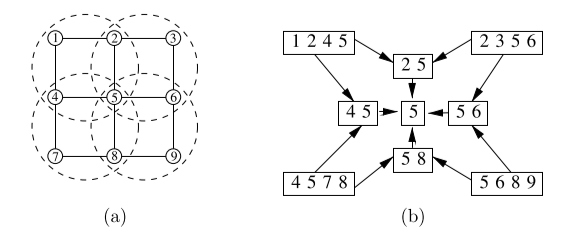
\includegraphics[width=.9\linewidth]{figure/4-5.PNG}
    \caption{
        (a) 叠加在 $3 \times 3$ 网格图上的 Kikuchi 簇。
        (b) 由 Kikuchi 簇给出的超图。
    }\label{fig:4-5}
\end{figure}

\subsection{广义信念传播}

原则上来说,变分问题 (4.53) 可以通过很多方法进行求解。
在这里我们描述一种基于 Lagrangian 的消息传递算法,这也是 Bethe 近似下的原始 Sum-product 算法的一种泛化。
这个方法的特点是消息只从父节点传递到子节点,也就是沿着超图的偏序集表示下的有向边传递。

在基于超树的变分问题 (4.53) 中,变量为每条超边 $h \in E$ 上的伪边际 $\tau_h$。
与前面对 Sum-product 算法的推导一样,这个优化问题的 Lagrangian 形式可以导出基于消息传递机制表示下的伪边际,其中的消息与 Lagrange 乘子有关。
原始问题有多种 Lagrangian 形式,从而可以导出多种消息传递算法。
在这里我们给出由 Yedidia et al. 推导的 Parent-to-child 形式的消息传递算法。

为了描述消息传递的更新机制,我们对给定的超边 $h$ 定义如下形式的后代集合(Descendants)与祖先集合(Ancestors):
\begin{equation}
    \mathcal{D}(h) := \{g \in E| g \subset h\}, \quad \mathcal{A}(h) := \{g \in E| g \supset h\}.
\end{equation}
例如,对于图 \ref{fig:4-4}(c) 中的超边 $h = (1245)$,我们有 $\mathcal{A}(h) = \emptyset, \mathcal{D}(h) = \{(25), (45), (5)\}$。
此外,我们定义 $\mathcal{D}^+(h) := \mathcal{D}(h) \cup \{h\}$ 以及 $\mathcal{A}^+(h) := \mathcal{A}(h) \cup \{h\}$。

给定一对超边 $(f, g)$,令 $M_{f \rightarrow g}(x_g)$ 代表从超边 $f$ 传递到超边 $g$ 的“消息”。
具体说来,这个消息是 $x_g$ 的状态空间上的一个函数(在离散情况下是一个多维数组)。
伪边际 $\tau_h$ 在这种 Parent-to-child 消息传递机制下的表示为:
\begin{equation}
    \tau_h(x_h) \propto \left[\prod_{g \in \mathcal{D}^+(h)}\psi_g(x_g; \theta)\right]\left[\prod_{g \in \mathcal{D}^+(h)}\prod_{f \in Par(g)/\mathcal{D}^+(h)}M_{f \rightarrow g}(x_g)\right], 
\end{equation}
式中 $\psi_g(x_g; \theta) = \exp(\theta(x_g))$。
伪边际 $\tau_h$ 的计算中包含了集合 $\mathcal{D}^+(h)$ 内每条超边 $g$ 的一个可计算函数 $\psi_g$。
此外,伪边际 $\tau_h$ 还需要从每条超边 $f \in Par(g)/\mathcal{D}^+(h)$ 中收集消息。
接下来我们通过对例 4.6 继续进行讨论来说明这种构造。

\begin{tcolorbox}
\begin{exam}[Kikuchi 近似下的 Parent-to-child 消息传递]

我们依旧采用图 \ref{fig:4-5} 中的 $3 \times 3$ 格点的 Kikuchi 近似来举例理解 Parent-to-child 消息传递机制。
首先考虑超边 $(1245)$,式 (4.56) 中的第一项是 $\mathcal{D}^+(1245)$ 中元素 $g$ 的可计算函数 $\psi_g$ 的乘积,本例中为 $\psi_{1245}\psi_{25}\psi_{45}\psi_5$。
然后考虑 $\mathcal{D}^+(1245)$ 中元素的父节点超边(但不包括 $\mathcal{D}^+(1245)$ 内部已有的超边)的消息的乘积。
图 \ref{fig:4-6}(a) 给出了相关示意,集合 $\mathcal{D}^+\{(1245)\}$ 由虚线椭圆中的超边给出。
在本例中,集合 $\bigcup_gPar(g)/\mathcal{D}^+(h)$ 为 $\{(2356), (4578)\}$,也就是 $(25), (45)$ 与 $(56), (58)$ 分别组合的父节点,这些超边也都是超边 $(5)$ 的父节点。
整体的结果如下:
\begin{align*}
    \tau_{1245} \propto &\psi_{12}'\psi_{14}'\psi_{25}'\psi_{45}'\psi_1'\psi_2'\psi_4'\psi_5' \\
    &\times M_{(2356)\rightarrow(25)}M_{(4578)\rightarrow(45)}M_{(56)\rightarrow 5}M_{(58)\rightarrow 5}.
\end{align*}
由于对称性,其他四个超边上的伪边际的表达式是类似的。
$\tau_{45}$ 和 $\tau_5$ 的表达式也可以通过类似的论证给出:
\begin{align*}
    \tau_{45} &\propto \psi_{45}'\psi_4'\psi_5'M_{(1245)\rightarrow(45)}M_{(4578)\rightarrow(45)}M_{(25)\rightarrow 5}M_{(56)\rightarrow 5}M_{(58)\rightarrow 5} \\
    \tau_5 &\propto \psi_5'M_{(45)\rightarrow 5}M_{(25)\rightarrow 5}M_{(56)\rightarrow 5}M_{(58)\rightarrow 5}.
\end{align*}

\end{exam}
\end{tcolorbox}

\begin{figure}[htbp]
    \centering
    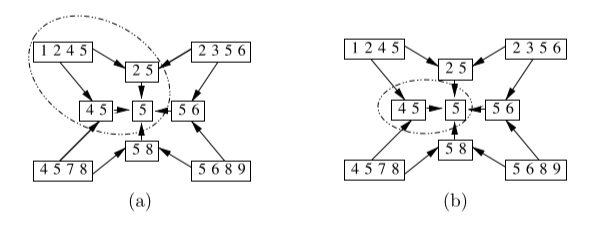
\includegraphics[width=.9\linewidth]{figure/4-6.PNG}
    \caption{
        Kikuchi 近似下的 Parent-to-child 消息传递机制示意。
        (a) 超边 $(1245)$ 的消息传递。
        后代集合 $\mathcal{D}^+\{(1245)\}$ 采用虚线椭圆框起来了。
        与 $\tau_{1245}$ 有关的父节点 包括集合 $\{(2356), (4578), (56), (58)\}$。
        (b) 超边 $(45)$ 的消息传递。
        后代集合 $\mathcal{D}^+\{(45)\}$ 同样采用虚线椭圆框起来了。
        相关的父节点集合为 $\{(1245), (4578), (25), (56), (58)\}$。
    }\label{fig:4-6}
\end{figure}

一般形式的 Sum-product 消息传递通过消息更新来保证 $\mathcal{L}(G)$ 中元素的边际化约束。
命题 4.2 的证明过程给出了消息更新的不动点满足 Lagrangian 公式的必要平稳条件。
关于一般化的 Sum-product 变体的细节可以在其他的论文中找到。

\section{期望传播算法}

在 Sum-product 算法的激励下,许多其他的消息传递算法也得到了发展。
例如 Minka 的 Expectation-propagation 算法族,相关的一类假定密度滤波方法(Assumed Density Filtering Methods),Expectation-consistent 推断,结构化 Summary-propagation 算法,以及 Opper 与 Winther 的自适应 TAP 方法。
这些算法通常是根据局部局匹配(Moment-matching)更新序列来定义的,是基于变分原理的个体更新,而不是整体逼近。
在本节中,我们将这些算法归纳到变分推理的框架之下,也就是证明它们是命题 3.4 中精确变分原理的特殊近似。

最早的假定密度滤波是在时间序列应用中发展起来的,最基本的模型就是图 \ref{fig:2-4} 所示的隐马尔可夫模型(HMM)。
我们之前已经讨论过,离散变量下的 HMM 的边际分布可以使用 Forward-backward 算法进行计算,这也是 Sum-product 算法的一个实例。
相似地,对于 Gauss-Markov 过程,Kalman 滤波可以计算 HMM 每个节点的均值与方差。
然而,对于一般化的连续变量隐马尔可夫模型而言,从节点 $t$ 传递给 $s$ 的消息 $M_{ts}$ 是一个实值函数,因此很难表示\footnote{
    Gaussian 情况是特例,因为它的消息函数总可以用均值和方差进行参数化表达,这也是 Kalman 滤波有效的基础。
}。假定密度滤波(ADF)的目的是为了绕过消息函数相关的计算困难,因此采用了消息函数的近似形式来进行操作,亦即利用某些合适的可计算类函数来对消息函数进行近似。
例如一般的连续消息可以近似为 Gaussian 消息。
如果采用 Kullback-Leibler 散度来度量接近度,那么计算消息近似的过程就能用 Moment-matching 操作来进行表示。

Minka 观察到 ADF 的基本思想可以不局限于马尔可夫链进而推广到任意图模型,这一见解构成了 Expectation-propagation(EP)算法族的基础。
与 ADF 一样,EP 及其相关算法通常利用 Moment-matching 操作来描述。
到目前为止,这些算法与 Bethe 近似之间的密切联系似乎并没有得到广泛的重视。
在本节中,我们将证明这些算法是求解命题 3.4 中精确变分原理的某些使用 Bethe-like 近似熵以及集合 $\mathcal{M}$ 上特定的凸外边界的松弛方法。
更具体地说,我们将证明 EP 的 Moment-matching 更新实际是求解优化问题的 Lagrangian 方法的一种特例,从而表明 EP 算法与 Belief-propagation 算法属于同一类变分方法。

\subsection{基于解耦项的近似熵}

我们首先基于对一个比较棘手的项式集合进行解耦的操作来给出一类一般的近似熵。
对给定的随机变量集合 $(X_1, \cdots, X_m) \in \mathbb{R}^m$,考虑将充分统计量进行如下分组:
\begin{equation}
    \underbrace{\phi := (\phi_1, \cdots, \phi_{d_T}),}_{\text{Tractable component}} \quad \underbrace{\Phi := (\Phi^1, \Phi^2, \cdots, \Phi^{d_I}),}_{\text{Intractable component.}}
\end{equation}
式中 $\phi_i$ 为单元统计量而 $\Phi^i$ 一般为多元统计量。
在下面的例子中我们会清楚地看到这个分组可以将相关的指数族分布的可处理分量与难处理分量分开。

我们需要为 $(\phi, \Phi)$ 的一些子集构建相关的指数族。
首先考虑容易处理的分量,向量值函数 $\phi: \mathcal{X}^m \rightarrow \mathbb{R}^{d_T}$ 具有对应的正则参数向量 $\theta \in \mathbb{R}^{d_T}$。
然后考虑难以处理的分量,对于每个 $i = 1, \cdots, d_I$,函数 $\Phi^i$ 将 $\mathcal{X}^m$ 映射到 $\mathbb{R}^b$,向量 $\tilde{\theta^i} \in \mathbb{R}^b$ 为相应的正则参数集。
总而言之,函数 $\Phi = (\Phi^1, \cdots, \Phi^{d_I})$ 将 $\mathcal{X}^m$ 映射到 $\mathbb{R}^{b\times d_I}$,相关的正则参数向量为 $\tilde{\theta} \in \mathbb{R}^{b\times d_I}$,可以被分组为 $\tilde{\theta} = (\tilde{\theta^1}, \tilde{\theta^2}, \cdots, \tilde{\theta^{d_I}})$。
这些充分统计量定义了如下指数族:
\begin{align}
    p(x; \theta, \tilde{\theta}) &\propto f_0(x)\exp(\langle\theta, \phi(x)\rangle)\exp(\langle\tilde{\theta}, \Phi(x)\rangle) \nonumber \\
    &= f_0(x)\exp(\langle\theta, \phi(x)\rangle)\prod_{i = 1}^{d_I}\exp(\langle\tilde{\theta^i}, \Phi^i(x)\rangle).
\end{align}
我们称任意具备 (4.58) 形式的密度 $p$ 属于 $(\phi, \Phi)$ 指数族。

接下来,我们定义如下基模型(Base Model):
\begin{equation}
    p(x; \theta, \vec{0}) \propto f_0(x)\exp(\langle\theta, \phi(x)\rangle), 
\end{equation}
在 $\tilde{\theta} = \vec{0}$ 的条件下难以处理的充分统计量 $\Phi$ 不起作用。
我们称任意具备 (4.59) 形式的分布 $p$ 属于 $\phi$ 指数族。
同样,对于任意 $i \in \{1, \cdots, d_I\}$,我们定义 $\Phi^i$ 增广分布(Augmented Distribution):
\begin{equation}
    p(x; \theta, \tilde{\theta^i}) \propto f_0(x)\exp(\langle\theta, \phi(x)\rangle)\exp(\langle\tilde{\theta^i}, \Phi^i(x)\rangle), 
\end{equation}
其中只引入了单项 $\Phi^i$,我们称任意具备 (4.60) 形式的分布 $p$ 属于 $(\phi, \Phi^i)$ 指数族。

对 $\phi, \Phi$ 进行 Tractable-Intractable 分组的基本前提是:
\begin{itemize}
    \item 第一,对于满足基本型 (4.59) 的分布(也就是 $\phi$ 指数族的成员)来说可以在多项式时间内精确计算出边际。
    \item 第二,对于任意 $i = 1, \cdots, d_I$,同样可以在多项式时间内精确计算满足基本型 (4.60) 的分布(也就是 $(\phi, \Phi^i)$ 指数族)的边际。
    \item 第三,对于全 $(\phi, \Phi)$ 指数族 (4.58) 而言很难执行精确计算,因为需要考虑所有项 $(\Phi^1, \Phi^2, \cdots, \Phi^{d_I})$。
\end{itemize}

\begin{tcolorbox}
\begin{exam}[混合模型的 Tractable-Intractable 分组]

我们以 Gaussian 混合模型为例来理解 (4.58) 的分配模式。
假设随机向量 $X \in \mathbb{R}^m$ 具有多元 Gaussian 分布,$N(0, \Sigma)$。
令 $\varphi(y; \mu, \Lambda)$ 表示分布为 $N(\mu, \Lambda)$ 的随机向量的密度,考虑以下两个成分的 GMM
\begin{equation}
    p(y| X = x) = (1-\alpha)\varphi(y; 0, \sigma_0^2I) + \alpha\varphi(y; x, \sigma_1^2I), 
\end{equation}
其中 $\alpha \in (0, 1)$ 代表混合权重,$\sigma_0^2$ 和 $\sigma_1^2$ 为方差,$I$ 为 $m \times m$ 的单位矩阵。

给定采样自混合密度 (4.61) 的 $n$ 个 i.i.d. 样本 $(y^1, y^2, \cdots, y^n)$,我们需要计算 $X$ 的后验分布的边际。
假设 $X$ 满足多元 Gaussian 先验 $X \sim N(0, \Sigma)$,使用 Bayes 定理可得后验形式为:
\begin{align}
    p(x|y^1, \cdots, y^n) &\propto \exp(-\frac{1}{2}x^T\Sigma^{-1}x)\prod_{i = 1}^np(y^i|X = x) \nonumber \\
    &= \exp(-\frac{1}{2}x^T\Sigma^{-1}x)\exp\left\{\sum_{i = 1}^n\log p(y^i|X = x)\right\}.
\end{align}

将这个模型转化为分组指数族 (4.58) 的形式,我们首先注意到 $\exp(-\frac{1}{2}x^T\Sigma^{-1}x)$ 能够用基本型 $f_0(x)\exp(\langle\theta, \phi(x)\rangle)$ 进行表示,因此有 $d_T = m$。
另一方面,我们对 $i = 1, \cdots, n$ 定义 $\Phi^i(x) := \log p(y^i|X = x)$。
应当指出的是这种定义是合理的,因为 $y^i$ 实际上是定值。
由以上定义可知 $\exp\{\sum_{i = 1}^n\log p(y^i|X = x)\}$ 实际就是式 (4.58) 中的乘积 $\prod_{i = 1}^{d_I}\exp(\langle\tilde{\theta^i}, \Phi^i(x)\rangle)$。
注意此处 $d_I = n, b = 1$,对于 $i = 1, \cdots, n$ 有 $\tilde{\theta^i} = 1$。

作为 $(\phi, \Phi)$ 指数族的一个例子,基础分布 $p(x; \theta, \vec{0}) \propto \exp(-\frac{1}{2}x^T\Sigma^{-1}x)$ 是一个多元 Gaussian,其边际可以在 $\mathcal{O}(m^3)$ 内精确计算出来。
同样地,对于 $i = 1, \cdots, n$,由 $\Phi^i$ 参数化表达的分布 (4.60) 与下式成正比:
\begin{equation}
    \exp(-\frac{1}{2}x^T\Sigma^{-1}x)[(1-\alpha)\varphi(y^i; 0, \sigma_0^2I)+\alpha\varphi(y^i; x, \sigma_1^2I)].
\end{equation}
这是一个具有两个成分的混合 Gaussian,因此也可以在立方时间内对边际进行精确计算。
然而,全分布 (4.62) 是一个具有 $2^n$ 个成分的混合 Gaussian,因此对边际进行精确计算的时间复杂度是问题规模的指数级。

\end{exam}
\end{tcolorbox}

回到主线,我们继续探索式 (4.58) 的一些性质。
作为一个指数族,其同样具有均值参数 $(\mu, \tilde{\mu}) \in \mathbb{R}^{d_T}\times\mathbb{R}^{d_I\times b}$,其中
\begin{equation*}
    \mu = \mathbb{E}[\phi(X)], \quad (\tilde{\mu}^1, \cdots, \tilde{\mu}^{d_I}) = \mathbb{E}[\Phi^1(X), \cdots, \Phi^{d_I}(X)].
\end{equation*}
作为一个指数族,命题 3.4 给出的一般变分原理同样适用。
变分原理 (3.45) 中的均值参数集合为
\begin{equation}
    \mathcal{M}(\phi, \Phi) := \{(\mu, \tilde{\mu})|(\mu, \tilde{\mu}) = \mathbb{E}_p[(\phi(X), \Phi(X))] \text{ for some } p\}, 
\end{equation}
熵(也就是负对偶函数)$H(\mu, \tilde{\mu}) = -A^*(\mu, \tilde{\mu})$。
我们的假设是,在全分布 (4.58) 下无法进行精确计算,因此均值空间 (4.64) 与熵函数的计算一定也存在相应的困难。
因此,我们现在根据分布的划分结构 (4.58) 来描述这些量的自然近似,从而得到一类 Expectation-propagation 算法。

与基分布 (4.59) 相关的均值参数集合为
\begin{equation}
    \mathcal{\phi} := \{\mu \in \mathbb{R}^{d_T}|\mu = \mathbb{E}_p[\phi(X)] \text{ for some density } p\}, 
\end{equation}
因此基分布也可以看做是一个 $d_T$ 维度的指数族。
根据命题 3.3,对于任意 $\mu \in \mathcal{M}^\circ(\phi)$,总是可以由一个指数族成员 $p_{\theta(\mu)}$ 导出。
此外,我们假设基分布容易计算,因此其熵函数 $H(\mu)$ 是可以直接得到的。
同样地,对于每一个 $i = 1, \cdots, d_I$,$\Phi^i$ 增广分布 (4.60) 也具有其均值参数空间 $\mathcal{M}(\phi, \Phi^i)$
\begin{equation}
    \{(\mu, \tilde{\mu}^i) \in \mathbb{R}^{d_T}\times\mathbb{R}^b| (\mu, \tilde{\mu}^i) = \mathbb{E}_p[(\phi(X), \Phi^i(X))] \text{ for some density } p\}.
\end{equation}
同理,对于任意 $(\mu, \tilde{\mu}^i) \in \mathcal{M}^\circ(\phi, \Phi^i)$,也都有一个 $(\phi, \Phi^i)$ 指数族成员可以得到这样的均值参数。
此外,因为 $\Phi^i$ 增广分布 (4.60) 容易计算,均值参数集合 $\mathcal{M}(\phi, \Phi^i)$ 以及熵函数 $H(\mu, \tilde{\mu}^i)$ 也是可以直接得到的。

有了这些基本概念,我们现在可以为集合 $\mathcal{M}(\phi, \Phi)$ 定义一个外边界。
给定某个均值参数候选集 $(\tau, \tilde{\tau}) \in \mathbb{R}^{d_T}\times\mathbb{R}^{d_I\times b}$,对任意 $i = 1, 2, \cdots, d_I$ 我们都定义一个坐标投影算子 $\Pi^i : \mathbb{R}^{d_T}\times\mathbb{R}^{d_I\times b} \rightarrow \mathbb{R}^{d_T}\times\mathbb{R}^b$:
\begin{equation*}
    (\tau, \tilde{\tau}) \xrightarrow{\Pi^i} (\tau, \tilde{\tau}^i) \in \mathbb{R}^{d_T}\times\mathbb{R}^b.
\end{equation*}
我们再定义集合
\begin{equation}
    \mathcal{L}(\phi; \Phi) := \{(\tau, \tilde{\tau})| \tau \in \mathcal{M}(\phi), \Pi^i(\tau, \tilde{\tau}) \in \mathcal{M}(\phi, \Phi^i) \forall i = 1, \cdots, d_I\}.
\end{equation}
注意有 $\mathcal{L}(\phi, \Phi)$ 为一个凸集,并且它也是原均值参数集合 $\mathcal{M}(\phi; \Phi)$ 的一个外边界。

我们现在给出熵函数的近似来适配结构 $\mathcal{L}(\phi; \Phi)$。
首先对于任意 $(\tau, \tilde{\tau}) \in \mathcal{L}(\phi, \Phi)$ 以及任意的 $i = 1, \cdots, d_I$,都有一个均值参数为 $(\tau, \tilde{\tau}^i)$ 的 $(\phi, \Phi^i)$ 指数族与之对应。
令 $H(\tau, \tilde{\tau}^i)$ 表示该指数族成员的熵。
同样地,根据 $\mathcal{L}(\phi; \Phi)$ 的定义有 $\tau \in \mathcal{M}(\phi)$,因此也存在一个均值参数为 $\tau$ 的 $\phi$ 指数族;我们将它的熵表示为 $H(\tau)$。
有了以上概念,我们定义如下的 Term-by-term 近似熵:
\begin{equation}
    H_{ep}(\tau, \tilde{\tau}) := H(\tau) + \sum_{l = 1}^{d_I}[H(\tau, \tilde{\tau}^l) - H(\tau)].
\end{equation}
结合近似熵与凸边界 (4.67) 可得优化问题
\begin{equation}
    \max_{(\tau, \tilde{\tau}) \in \mathcal{L}(\phi; \Phi)}\{\langle\tau, \theta\rangle + \langle\tilde{\tau}, \tilde{\theta}\rangle + H_{ep}(\tau, \tilde{\tau})\}.
\end{equation}
该优化问题即为命题 3.4 给出的精确变分原理的针对 $(\phi, \Phi)$ 指数族 (4.58) 的近似版本,这也是 Expectation-propagation 算法的基础。
如下面的例子所示,该优化问题与 Bethe 变分原理也关系密切。

\begin{tcolorbox}
\begin{exam}[Sum-product 与 Bethe 近似]

为了便于理解,我们现在从变分原理 (4.69) 的角度来考虑 Bethe 近似。
更具体地说,我们将从 Term-by-term 近似熵 (4.68) 中导出 Bethe 近似熵 (4.14),同时从 $\mathcal{M}(\phi, \Phi)$ 的凸外界 (4.67) 中导出式 (4.7) 中的基于树的外边界 $\mathcal{L}(G)$。

考虑一个基于无向图 $G = (V, E)$ 的成对 MRF,其每个节点 $s \in V$ 对应的变量离散为 $X_s \in \{0, 1, \cdots, r_s-1\}$;
和我们先前所看到的一样,它也可以借助指示函数和标准过完备参数化 (3.34) 表示为如 (4.1) 形式的指数族。
采用式 (4.69) 的观点,我们将充分统计量进行如下划分。
与节点相关的充分统计量定义为可处理集,与连边相关的统计量定义为难处理集。
借助式 (4.2) 中定义的函数 $\theta_s$ 和 $\theta_{st}$,基分布 (4.59) 可以表示为
\begin{equation}
    p(x; \theta_1, \cdots, \theta_m, \vec{0}) \propto \prod_{s \in V}\exp(\theta_s(x_s)).
\end{equation}
在这个例子中,$\Phi^i$ 项与函数 $\theta_{st}$ 相关联,也就是索引 $i$ 取值自图的连边集合。
对于每条边 $(u, v)$,$\Phi^{uv}$ 增广分布 (4.60) 具有以下形式:
\begin{equation}
    p(x; \theta_1, \cdots, \theta_m, \theta_{uv}) \propto [\prod_{s \in V}\exp(\theta_s(x_s))]\exp(\theta_{us}(x_u, x_v)).
\end{equation}

标准过完备表示的均值参数为 Singleton 和 Pairwise 的边际分布,我们使用 $(\tau_s, s \in V)$ 与 $\tau_{uv}$ 分别进行表示。
基分布的熵只取决于 Singleton 的边际,借助 (4.70) 的乘积结构,其简单形式为
\begin{equation*}
    H(\tau_1, \cdots, \tau_m) = \sum_{s \in V}H(\tau_s), 
\end{equation*}
其中 $H(\tau_s) = -\sum_{x_s}\tau_s(x_s)\log\tau_s(x_s)$ 就是边际分布的熵。
同样地,由于增广分布 (4.71) 只在无环图上添加并分解了一条边,其熵具有显式形式
\begin{align*}
    H(\tau_1, \cdots, \tau_m, \tau_{uv}) &= \sum_{s \in V}H(\tau_s) + [H(\tau_{uv}) - H(\tau_u) - H(\tau_v)] \\
    &= \sum_{s \in V}H(\tau_s) - I(\tau_{uv}), 
\end{align*}
其中 $H(\tau_{uv}) := -\sum_{x_u, x_v}\tau_{uv}(x_u, x_v)\log\tau_{uv}(x_u, x_v)$ 为联合熵,$I(\tau_{uv}) := H(\tau_u) + H(\tau_v) - H(\tau_{uv})$ 为互信息。
将这些碎片结合在一起,我们可以发现 Term-by-term 近似熵 (4.68) 在这个特定的问题下的形式为:
\begin{equation*}
    H_{ep}(\tau) = \sum_{s \in V}H(\tau_s) - \sum_{(s, t) \in E}I_{st}(\tau_{st}), 
\end{equation*}
这也就是式 (4.14) 所定义的 Bethe 近似熵。

接下来,我们将展示由式 (4.67) 定义的外边界 $\mathcal{L}(\phi; \Phi)$ 是如何导出 $\mathbb{L}(G)$ 的。
考虑局部候选边际分布集合
\begin{equation*}
    \tau = (\tau_s, s \in V; \tau_{st}, (s, t) \in E).
\end{equation*}
在现有的设定里,集合 $\mathcal{M}(\phi)$ 对应于分解分布下所有可实现边际 $(\tau_s, s \in V)$ 的集合,因此包含关系 $(\tau_s, s \in V) \in \mathcal{M}(\phi)$ 与非负性约束 $\forall s \in V: \tau_s(x_s) \geq 0$ 以及局部归一化约束
\begin{equation}
    \forall s \in V: \sum_{x_s}\tau_s(x_s) = 1
\end{equation}
等价。
注意到索引 $i$ 取值于图的连边集合;以 $i = (u, v)$ 为例,投影边际 $\Pi^{uv}(\tau)$ 为 $(\tau_1, \cdots, \tau_m, \tau_{uv})$。
集合 $\mathcal{M}(\phi; \Phi^{uv})$ 为所有这种形式的全局一致边际,并且与边际多面体 $\mathbb{M}(G_{uv})$ 等价,其中 $G_{uv}$ 表示仅有一条边 $(u, v)$ 的图。
由于这个图是树结构的,因此包含关系 $\Pi^{uv}(\tau) \in \mathcal{M}(\phi; \Phi^{uv})$ 与让 $\Pi^{uv}(\tau)$ 满足非负性约束以及局部归一化约束 (4.72) 条件,也就是边际化条件
\begin{equation*}
    \sum_{x_v}\tau_{uv}(x_u, x_v) = \tau_u(x_u), \quad \sum_{x_u}\tau_{uv}(x_u, x_v) = \tau_v(x_v)
\end{equation*}
等价。
因此,当 $(u, v)$ 取遍图的连边集合 $E$ 上时,包含关系 $\Pi^{uv}(\tau) \in \mathcal{M}(\phi; \Phi^{uv})$ 的全集给出了与式 (4.7) 定义的一阶松弛约束集合 $\mathbb{L}(G)$ 相同的条件。

\end{exam}
\end{tcolorbox}

\subsection{矩匹配的最优性}

回到主线上,我们现在推导解决 Expectation-propagation 变分原理 (4.69) 的 Lagrangian 方法。
我们将会展示这些 Lagrangian 更新实际上就是 Moment-matching,因此也包含了一般的 Expectation-propagation 更新。

我们基于以下两个基本步骤进行 Lagrangian 形式化:
\begin{itemize}
    \item 首先,我们扩大要进行优化的伪均值参数空间,使得定义 $\mathcal{L}(\phi; \Phi)$ 的原始约束解耦。
    \item 然后,我们用 Lagrange 乘子作为罚项引入新的约束,以使得最后的约束就是 $\mathcal{L}(\phi; \Phi)$ 中的成员所需要的。
\end{itemize}
首先开始增广步骤,我们将向量 $\tau \in \mathbb{R}^{d_T}$ 复制 $d_I$ 次,得到 $d_I$ 个新的向量 $\eta^i \in \mathbb{R}^{d_T}$ 并引入新的约束 $\forall i = 1, \cdots, d_I: \eta^i = \tau$。
由此可得到伪均值参数集合
\begin{equation*}
    \{\tau, (\eta^i, \tilde{\tau}^i), i = 1, \cdots, d_I\} \in \mathbb{R}^{d_T}\times(\mathbb{d_T}\times\mathbb{R}^b)^{d_I}, 
\end{equation*}
然后我们利用这些伪均值参数重新组织变分原理 (4.69):
\begin{equation}
    \max_{\{\tau, (\eta^i, \tilde{\tau}^i)\}}\left\{\langle\tau, \theta\rangle + \sum_{i = 1}^{d_I}\langle\tilde{\tau}^i, \tilde{\theta}^i\rangle + \underbrace{H(\tau) + \sum_{i = 1}^{d_I}[H(\eta^i, \tilde{\tau}^i) - H(\eta^i)]}_{F(\tau; (\eta^i, \tilde{\tau}^i))} \right\}, 
\end{equation}
其约束为 $\forall i = 1, \cdots, d_I: (\eta^i, \tilde{\tau}^i) \in \mathcal{M}(\phi; \Phi^i)$ 以及
\begin{equation}
    \tau = \eta^i \quad \forall i = 1, \cdots, d_I.
\end{equation}

现在让我们考虑一个特殊的迭代方案来解决问题 (4.73)。
特别地,对于每一个 $i = 1, \cdots, d_I$,定义一个与约束 $\tau = \eta_i$ 相关联的 Lagrange 乘子向量 $\lambda^i \in \mathbb{R}^{d_T}$。
我们可以得到 Lagrangian 函数
\begin{equation}
    L(\tau; \lambda) = \langle\tau, \theta\rangle + \sum_{i = 1}^{d_I}\langle\tilde{\tau}^i, \tilde{\theta}^i\rangle + F(\tau; (\eta^i, \tilde{\tau}^i)) + \sum_{i = 1}^{d_I}\langle\lambda^i, \tau-\eta^i\rangle.
\end{equation}
这个 Lagrangian 只是一部分,因为我们强迫满足约束 $\tau \in \mathcal{\phi}$ 以及 $(\eta^i, \tilde{\tau}^i) \in \mathcal{M}(\phi; \Phi^i)$。

考虑优化问题 (4.73) 的一个最优解 $\{\tau, (\eta^i, \tilde{\tau}^i), i = 1, \cdots, d_I\}$,这个解满足:
(a) 向量 $\tau$ 属于相对内点集 $\mathcal{M}^\circ(\phi)$,
(b) 对于每个 $i = 1, \cdots, d_I$,向量 $(\eta^i, \tilde{\tau}^i)$ 属于相对内点集 $\mathcal{M}^\circ(\phi; \Phi^i)$。
任何解都必须满足部分 Lagrangian (4.75) 相关的零梯度条件,也就是
\begin{subequations}
\begin{align}
    \nabla_{\tau}L(\tau; \lambda) &= 0, \\
    \nabla_{(\eta^i, \tilde{\tau}^i)}L(\tau; \lambda) &= 0 \quad \text{for } i = 1, \cdots, d_I, \\
    \nabla_{\lambda}L(\tau; \lambda) &= 0.
\end{align}
\end{subequations}

由于向量 $\tau$ 属于 $\mathcal{M}^\circ(\phi)$,因此它给定了 $\phi$ 指数族中的一个分布。
通过计算 Lagrangian 条件 (4.76a) 并进行简单的代数运算,我们发现这个指数族分布可以采用原始的参数向量 $\theta$ 以及 Lagrange 乘子 $\lambda$ 写为如下形式:
\begin{equation}
    q(x; \theta, \lambda) \propto f_0(x)\exp\left\{\langle\theta+\sum_{i = 1}^{d_I}\lambda^i, \phi(x)\rangle\right\}.
\end{equation}

同样地,对于每个 $i = 1, \cdots, d_I$,向量 $(\tau, \tilde{\tau}^i)$ 属于 $\mathcal{M}^\circ(\phi; \Phi^i)$,它也给定了 $(\phi, \Phi^i)$ 指数族中的一个分布。
对条件 (4.76b) 进行计算可知该分布可以表示为
\begin{equation}
    q^i(x; \theta, \tilde{\theta}^i, \lambda) \propto f_0(x)\exp(\langle\theta+\sum_{l \neq i}\lambda^l, \phi(x)\rangle + \langle\tilde{\theta}^i, \Phi^i(x)\rangle).
\end{equation}

最后的 Lagrangian 条件 (4.76c) 保证约束 (4.74) 得到满足。
注意到 $\tau = \mathbb{E}_q[\phi(X)]$ 以及 $\eta^i = \mathbb{E}_{q^i}[\phi(X)]$,这些约束可以得到 Moment-matching 条件
\begin{equation}
    \int q(x; \theta, \lambda)\phi(x)\nu(dx) = \int q^i(x; \theta, \tilde{\theta}^i, \lambda)\phi(x)\nu(dx), 
\end{equation}
对于 $i = 1, \cdots, d_I$ 成立。

基于式 (4.77),(4.78) 以及 (4.79),我们得到了 Expectation-propagation 更新,总结如图 \ref{fig:4-7} 所示。
可以看到算法的定义是合理的,因为对于任何可实现的均值参数 $\tau$,式 (4.81) 总会有一个解 $\lambda^{i(n)}$。
通过考虑由 $(\lambda^{i(n)}, \phi)$ 所定义的 $d_T$ 维度指数族,然后应用命题 3.3 就可以得到这个事实。
此外,这些 EP 更新的任何不动点都满足 (4.73) 优化所给出的 Lagrangian 条件。
基于这一点,我们提出一个重要结论,也就是假设优化问题 (4.73) 最少有一个最优点,那么 EP 更新的不动点一定存在。
与 Sum-product 算法与 Bethe 变分原理一样,EP 更新在一般情况下不能保证收敛。
然而,开发至少能找到变分问题 (4.73) 或等价的 (4.69) 的局部最优解的收敛算法相对简单,沿着为普通 Bethe 变分问题或其凸型版本开发的收敛算法的思路或许就能得到。

\begin{figure}[htbp]
    \textbf{Expectation-propagation (EP) 更新:}
    
    (1) 在 $n = 0$ 次迭代时,初始化 Lagrange 乘子向量 $(\lambda^1, \cdots, \lambda^{d_I})$。 
    
    (2) 在 $n = 1, 2, \cdots$ 的每次迭代中选择某个索引 $i(n) \in \{1, \cdots, d_I\}$,然后
        
    \quad (a) 使用式 (4.78) 构建增广分布 $q^{i(n)}$ 并且计算均值参数
        \begin{equation}
            \eta^{i(n)} := \int q^{i(n)}(x)\phi(x)\nu(dx) = \mathbb{E}_{q^{i(n)}}[\phi(X)].
        \end{equation}
    
    \quad (b) 使用式 (4.77) 构建基分布 $q$ 并且调整 $\lambda^{i(n)}$ 以满足 Moment-matching 条件
        \begin{equation}
            \mathbb{E}_q[\phi(X)] = \eta^{i(n)}.
        \end{equation}
    \caption{
        Expectation-propagation 更新的相关步骤。
        这是解决类 Bethe 问题 (4.73) 或等价的 (4.69) 的一种 Lagrangian 算法。
    }\label{fig:4-7}
\end{figure}

从更高的角度来看,一些关键要素如下:
在变分框架中,Expectation-propagation 算法是基于类 Bethe 的近似熵 (4.68) 以及均值参数集合的一个特定凸外界 (4.67)。
此外,EP 算法中的 Moment-matching 步骤来自于尝试解决变分原理 (4.69) 的一种 Lagrangian 方法。

最后,我们举例说明图 \ref{fig:4-7} 中算法的具体形式:

\begin{tcolorbox}
\begin{exam}[作为 Moment-matching 的 Sum-product]
    作为例 4.9 的后续,我们现在展示图 \ref{fig:4-7} 中的更新式 (4.80) 与 (4.81) 得到 Sum-product 更新的过程。
    在这个例子中,索引 $i$ 取值于图的连边集合。
    与 $i = (u, v)$ 相关的 Lagrange 乘子为 $(\lambda_{uv}(x_v), \lambda_{vu}(x_u))$。
    基分布 (4.77) 采用这些量可以写为
    \begin{align}
        q(x; \theta, \lambda) &\propto \prod_{s \in V}\exp(\theta_s(x_s))\prod_{(u, v) \in E}\exp(\lambda_{uv}(x_v)+\lambda_{vu}(x_u)) \nonumber \\
        &= \prod_{s \in V}\exp(\theta_s(x_s) + \sum_{t \in N(s)}\lambda_{ts}(x_s)), 
    \end{align}
    或者更简洁点,$q(x; \theta, \lambda) \propto \prod_{s \in V}\tau_s(x_s)$,其中我们定义伪边际
    \begin{equation*}
        \tau_s(x_s) \propto \exp(\theta_s(x_s)+\sum_{t \in N(s)}\lambda_{ts}(x_s)).
    \end{equation*}
    值得注意的是 Singleton 伪边际 $\tau_s$ 与由命题 4.2 得到的 Sum-product 表达式 (4.23) 之间的相似性。
    同样,当 $l = (u, v)$,增广分布 (4.78) 可以写为
    \begin{align}
        q^{(u, v)}(x; \theta, \lambda) &\propto q(x; \theta, \lambda)\exp(\theta_{uv}(x_u, x_v) - \lambda_{vu}(x_u) - \lambda_{uv}(x_v)) \nonumber \\
        &= [\prod_{s \in V}\tau_s(x_s)]\exp(\theta_{uv}(x_u, x_v)-\lambda_{vu}(x_u)-\lambda_{uv}(x_v)).
    \end{align}

    现在考虑更新式 (4.80) 与 (4.81)。
    如果 $i = (u, v)$,那么更新式 (4.80) 与计算分布 (4.83) 的 Singleton 边际等价。
    更新式 (4.81) 规定 Lagrange 乘子 $\lambda_{uv}(x_v)$ 与 $\lambda_{vu}(x_u)$ 必须得到调整以使得分布 (4.82) 的边际 $\{\tau_u, \tau_v\}$ 和这些边际相匹配。
    通过一些代数运算,这些不动点条件可以得到在边 $(u, v)$ 上的 Sum-product 更新,其中的消息是由指数化的 Lagrange 乘子给出的 $M_{uv}(x_v) = \exp(\lambda_{uv}(x_v))$。
\end{exam}
\end{tcolorbox}

从 Term-by-term 的观点来看,Sum-product 算法使用了基分布的乘积(参见式 (4.70))。
一个很自然的拓展是考虑具有更多结构的基分布。

\begin{tcolorbox}
\begin{exam}[树结构的 EP]
    我们将通过导出树结构的 EP 算法来解释这个想法,并将其应用在具有图结构 $G = (V, E)$ 的成对 MRF 上。
    我们使用与例 4.9 以及 例 4.10 相同的设定和参数化形式。
    给定这个图的某个生成树 $T = (V, E(T))$,基分布 (4.59) 为
    \begin{equation}
        p(x; \theta, \vec{0}) \propto \prod_{s \in V}\exp(\theta_s(x_s))\prod_{(s, t) \in E(T)}\exp(\theta_{st}(x_s, x_t)).
    \end{equation}
    在这个例子中,索引 $i$ 取值 $(u, v) \in E/E(T)$;
    给定边 $(u, v)$,$\Phi^{uv}$ 增广分布 (4.60) 可以通过添加项 $\theta_{uv}$ 得到:
    \begin{equation}
        p(x; \theta, \theta_{uv}) \propto p(x; \theta, \vec{0})\exp(\theta_{uv}(x_u, x_v)).
    \end{equation}

    我们现在描述集合 $\mathcal{M}(\phi, \Phi)$,$\mathcal{M}(\phi)$ 以及 $\mathcal{M}(\phi, \Phi^i)$ 在这种设定下的类比。
    首先,如例 4.9 所示,与全模型 (4.58) 相应的均值参数子向量为
    \begin{equation*}
        \mu := (\mu_s, s \in V; \mu_{st}, (s, t) \in E).
    \end{equation*}
    据此,$\mathcal{M}(\phi, \Phi)$ 的类比就是边际多面体 $\mathbb{M}(G)$。
    其次,如果我们使用树结构分布 (4.84) 作为基分布,相关均值参数的子向量为
    \begin{equation*}
        \mu(T) := (\mu_s, s \in V; \mu_{st}, (s, t) \in E(T)).
    \end{equation*}
    集合 $\mathcal{M}(\phi)$ 的类比就是边际多面体 $\mathbb{M}(T)$,或者等价的 —— 根据命题 4.1 —— 为集合 $\mathbb{L}(T)$。
    最后,如果我们使用边 $i = (u, v) \notin E(T)$,那么集合 $\mathcal{M}(\phi, \Phi^i)$ 的类比就是边际多面体 $\mathbb{M}(T \cup (u, v))$。

    集合 $\mathcal{L}(\phi; \Phi)$ 的类比比较有趣,我们将其称为边际多面体 $\mathbb{M}(G)$ 的 tree-EP 外界。
    它包含向量 $\tau = (\tau_s, s \in V; \tau_{st}, (s, t) \in E)$,这些向量满足
    \begin{itemize}
        \item[(a)] 包含关系 $\tau(T) \in \mathbb{M}(T)$ 成立,
        \item[(b)] 对于所有 $(u, v) \notin T$,包含关系 $(\tau(T), \tau_{uv}) \in \mathbb{M}(T \cup (u, v))$ 成立。
    \end{itemize}
    可以看到这么定义的集合含于 $\mathbb{L}(G)$:特别地,条件 $\tau(T) \in \mathbb{M}(T)$ 保证了与树结构相应的所有边际分布的非负性,归一性以及边际性,并且包含关系 $(\tau(T), \tau_{uv}) \in \mathbb{M}(T \cup (u, v))$ 保证了 $\tau_{uv}$ 是非负的,同时也满足与 $\tau_u$ 与 $\tau_v$ 之间的边际化关系。
    对于带环图,tree-EP 外边界严格含于 $\mathbb{L}(G)$;例如,当应用于三节点的单环 $C_3$ 上时,tree-EP 外边界和边际多面体等价。
    但是如例 4.1 所示,集合 $\mathbb{M}(C_3)$ 严格含于 $\mathbb{L}(C_3)$。
    
    tree-EP 相应的近似熵 $H_{ep}$ 很容易定义。
    给定在 tree-EP 外边界中的伪均值参数 $\tau$ 的候选集合,我们定义与基分布 (4.84) 相关的树结构熵
    \begin{equation}
        H(\tau(T)) := \sum_{s \in V}H(\tau_s) - \sum_{(s, t) \in E(T)}I_{st}(\tau_{st}).
    \end{equation}
    同样,对于每条边 $(u, v) \notin E(T)$,我们定义与增广分布 (4.85) 相对应的熵 $H(\tau(T), \tau_{uv})$;
    与基分布不同,这个熵没有精确形式(因为图不是联合树形式),但是它也很容易计算。
    tree-EP 近似熵的形式如下:
    \begin{equation*}
        H_{ep}(\tau) = H(\tau(T)) + \sum_{(u, v) \notin E(T)}[H(\tau(T), \tau_{uv}) - H(\tau(T))].
    \end{equation*}

    最后,我们导出 tree-EP 的 Moment-matching 更新式 (4.80) 与 (4.81)。
    对于每条边 $(u, v) \notin E(T)$,令 $\lambda^{uv}(T)$ 表示 Lagrange 乘子向量,与 $\tau(T)$ 的维度相同,再令 $\phi(x; T)$ 表示与 $T$ 相关的充分统计量的子集。
    优化后的基分布 (4.77) 可以使用原始基分布 (4.84) 和这些 Lagrange 乘子重新写为
    \begin{equation*}
        q(x; \theta, \lambda) \propto p(x; \theta, \vec{0})\prod_{(u, v) \notin E(T)}\exp(\langle\lambda^{uv}(T), \phi(x; T)\rangle).
    \end{equation*}
    如果边 $(u, v)$ 被加进去,增广分布 (4.78) 可以重新写为
    \begin{equation*}
        q^{uv}(x; \theta, \lambda) \propto p(x; \theta, \vec{0})\exp(\theta_{uv}(x_u, x_v))\prod_{(s, t) \neq (u, v)}\exp(\langle\lambda^{uv}(T), \phi(x; T)\rangle).
    \end{equation*}
    对于一个给定的边 $(u, v) \notin E(T)$,Moment-matching 步骤 (4.81) 与在分布 $q^{uv}(x; \theta, \lambda)$ 下为连边 $(s, t) \in E(T)$ 计算 Singleton 边际与 Pairwise 边际有关。
    步骤 (4.81) 与更新 Lagrange 乘子 $\lambda^{uv}(T)$ 以使得对于所有节点 $s \in V$ 以及连边 $(s, t) \in E(T)$ 而言 $q(x; \theta, \lambda)$ 所给出的边际与 $q^{uv}(x; \theta, \lambda)$ 所给出的相一致。
\end{exam}
\end{tcolorbox}

之前的例子都只考虑了离散随机变量;我们现在转向考虑首次出现在例 4.8 中的带有连续变量的混合模型。

\begin{tcolorbox}
\begin{exam}[Gaussian 混合模型的 EP]
    重新回忆指数族形式的混合模型表达式 (4.62),其包括基础的势函数 $\phi(x) = (x; xx^T)$ 以及对于 $i = 1, \cdots, n$ 的辅助项 $\Phi^i(x) = \log p(y^i|x)$。
    现在转向多种均值参数空间的类比,集合 $\mathcal{M}(\phi; \Phi)$ 是 $\mathbb{R}^m \times \mathcal{S}_+^m \times \mathbb{R}^n$ 的子集,相应的全局可实现均值参数空间被划分为
    \begin{equation*}
        (\mathbb{E}[X]; \mathbb{E}[XX^T]; \mathbb{E}[\log p(y^i|X)], i = 1, \cdots, n).
    \end{equation*}
    注意 $(y^1, y^2, \cdots, y^n)$ 为已观测量,因此在整个推导过程中保持不变。

    集合 $\mathcal{M}(\phi)$ 是 $\mathbb{R}^m\times\mathcal{S}_+^m$ 的一个子集,与例 3.7 给出的一个多元 Gaussian 的均值参数空间相关。
    对于 $i = 1, \cdots, n$,约束集合 $\mathcal{M}(\phi; \Phi^i)$ 是 $\mathbb{R}^m\times\mathcal{S}_+^m\times\mathbb{R}$ 的一个子集,与具有如下划分形式的所有全局可实现的均值参数集合相关
    \begin{equation*}
        (\mathbb{E}[X], \mathbb{E}[XX^T], \mathbb{E}[\log p(y^i|X)]).
    \end{equation*}

    现在转向考虑多种熵函数,基本项是多元 Gaussian 的熵 $H(\mu)$,其中 $\mu$ 表示 $(\mathbb{E}[X], \mathbb{E}(XX^T))$;
    相似地,增广项 $H(\mu, \tilde{\mu}^i)$ 是具有充分统计量 $(\phi(x), \log p(y^i|x))$ 的指数族成员的熵,均值参数为 $(\mu, \tilde{\mu}^i)$,其中 $\tilde{\mu}^i = \mathbb{E}[\log p(y^i|X)]$。
    我们可以使用这些量定义变分原理 (4.69) 的一个类比。

    现在转向考虑 Moment-matching 步骤 (4.80) 与 (4.81),Gaussian-mixture EP 算法的 Lagrangian 形式可以采用 $n$ 个矩阵-向量 Lagrange 乘子对来构建
    \begin{equation*}
        (\lambda^i, \Lambda^i) \in \mathbb{R}^m \times \mathbb{R}^{m \times m}, i = 1, \cdots, n,
    \end{equation*}
    每一个都对应一个增广分布。
    由于 $X \sim N(0, \Sigma)$,优化基分布 (4.77) 可以采用 $\Sigma^{-1}$ 与 Lagrange 乘子写为
    \begin{equation}
        q(x; \Sigma; (\lambda, \Lambda)) \propto \exp\left\{\langle\sum_{i = 1}^n\lambda^i, x\rangle+\langle\langle-\frac{1}{2}\Sigma^{-1}+\sum_{i = 1}^n\Lambda^i, xx^T\rangle\rangle\right\}.
    \end{equation}
    值得指出的是,这是一个简单的多元 Gaussian 分布。
    对于任意 $i \in \{1, 2, \cdots, d_I\}$ 相应的增广分布 (4.78) $q^i$ 形式如下:
    \begin{equation}
        f_0(x)\exp\{\langle\sum_{l \neq i}\lambda^l, x\rangle+\langle\langle-\frac{1}{2}\Sigma^{-1}+\sum_{l \neq i}\Lambda^l, xx^T\rangle\rangle+\langle\tilde{\theta}_i, \log p(y^i|x)\rangle\}.
    \end{equation}
    有了这些条件,步骤 (4.80) 就与在分布 (4.88) 下计算均值参数 $(\mathbb{E}_{q^i}[X], \mathbb{E}_{q^i}[XX^T])$ 相关,步骤 (4.81) 就与调整多元 Gaussian (4.87) 以使其具有这些均值参数相关。
    这些 Moment-matching 更新的不动点满足对精确变分原理的类 Bethe 近似进行最优求解的必要的 Lagrangian 条件。

    我们推荐读者进一步阅读 Minka 与 Seeger 的相关工作,以了解更多有关 Gaussian-mixture EP 算法及其性质的细节。
\end{exam}
\end{tcolorbox}
\chapter{平均场方法}

本章我们讨论平均场方法(Mean Field Methods)。
以本书的角度来看,平均场方法实际上是针对精确变分原理 (3.45) 的一种特定近似。
更准确地说,3.7 小节讨论过变分原理 (3.45) 的两个基础性难点:
约束集合 $\mathcal{M}$ 的性质不怎么好,对偶函数 $A^*$ 也没有解析形式。
平均场方法的核心思想很简单:我们只在所有可能分布的一个子集上进行优化,在这个子集上 $\mathcal{M}$ 和 $A^*$ 都比较简单。
在本章中,我们把这种分布叫做“可以驾驭的(tractable)”,其中最简单的选择就是乘积分布族,这也就是朴素平均场方法所考虑的。
高阶的平均场方法则是考虑具有更多结构性质的 tractable 分布。

\section{可驾驭族}




\end{document}